% This part is the latex header. It defines what kind of document this will be and 
% says which packages to use. Packages let you include different kind of formats
% and templates in the document. 
\documentclass[11pt]{article} % document type - other options are journal or book?
\usepackage[pdftex]{graphicx} % package to import figures
\usepackage{float} % used for placing figures - H
\usepackage{hyperref} % used for including links (hyper links)
\usepackage{enumerate} % used for making lists
\usepackage[margin=1cm]{geometry}
\usepackage{tabularx}
\usepackage{booktabs}
\usepackage{amsmath}
\usepackage[version=3]{mhchem} 
\usepackage{siunitx}

% math packages
\usepackage{amssymb}
\usepackage{amsmath}

\pagestyle{headings}
\topmargin -0.5in
\oddsidemargin 0.0in
\textwidth 6.5in
\textheight 9.0in

% declare the title, date and author
\title{Radial Bias Pilot 1}
\date{July 21, 2021}
\author{Rania Ezzo}

% This is where the actual document starts
\begin{document}
\maketitle
\tableofcontents


\section{Experiment Description of Pilot 1}
To compare discriminability for radial motion directions compared to tangential motion directions with 1D drifting gratings at 8 polar angle locations at 7 deg eccentricity. A total of 4 motion directions will be per location, 2 radial (inwards and outwards) and 2 tangential.

\subsection{Parameters}
Eccentricity from central fixation: 7 degrees
\\
Locations tested (polar angle relative to fixation): 0-315 degrees in 45 degree increments
\\
Stimulus: sine wave gratings w/ 0.4 deg sigma gaussian mask
\\
Stimulus spatial frequency: 1 c/deg
\\
Stimulus drift speed: 8 deg/s
\\
Stimulus contrast: 50\% contrast per grating + gaussian mask
\\
Stimulus aperature diameter: 2.5 deg
\\
Black circular aperature was put onto screen to avoid perceptual artifacts from screen edges
\\
Aborts trials that have breaks in fixation during stimulus presentation (stimulus\_start - 300 ms TO stimulus\_end)
\\
Number of subjects: 5

\subsection{Subject Instructions}
For each of the following trials, a fixation dot will appear on the screen. A drifting pattern will appear at some distance from the center. Your task is to determine whether the pattern is drifting clockwise or counterclockwise relative to the reference.
\\
Please remain fixated on the dot throughout the trials.
\\
Press the RIGHT ARROW for clockwise direction.
\\
Press the LEFT ARROW for counterclockwise direction.

\subsection{Experimental Design}
The pilot uses a 2AFC paradigm, within a block each trial includes a drifting grating presented at 1 of 4 possible positions, while the subject maintains fixation at the central dot. A method of constant stimuli is used which is set based on the performance of the training session (see Methods). The angular values added to the internal reference frame is chosen at random from the following constants [-8, -4, -2, -1, -0.5, 0.5, 1, 2, 4, 8] -- logarithmic spacing from 0.5 to 8. The observer must determine whether the direction of motion if clockwise or counterclockwise relative to the internal reference. The sequence of each trial for the 4 motion standards (specific to diagonal locations) at one location is depicted below:

\begin{figure}[H]
\centering % centers the figure
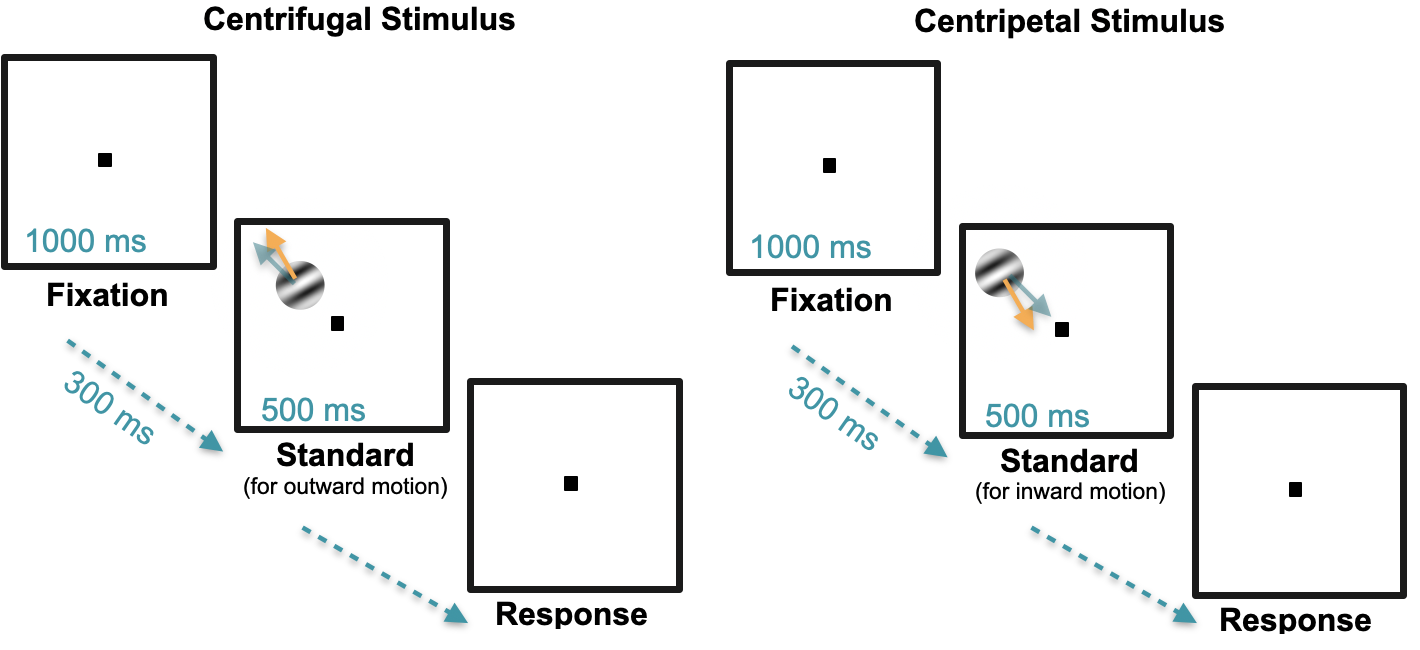
\includegraphics[scale=.4]{Images/Radial_sequence.png}
\\
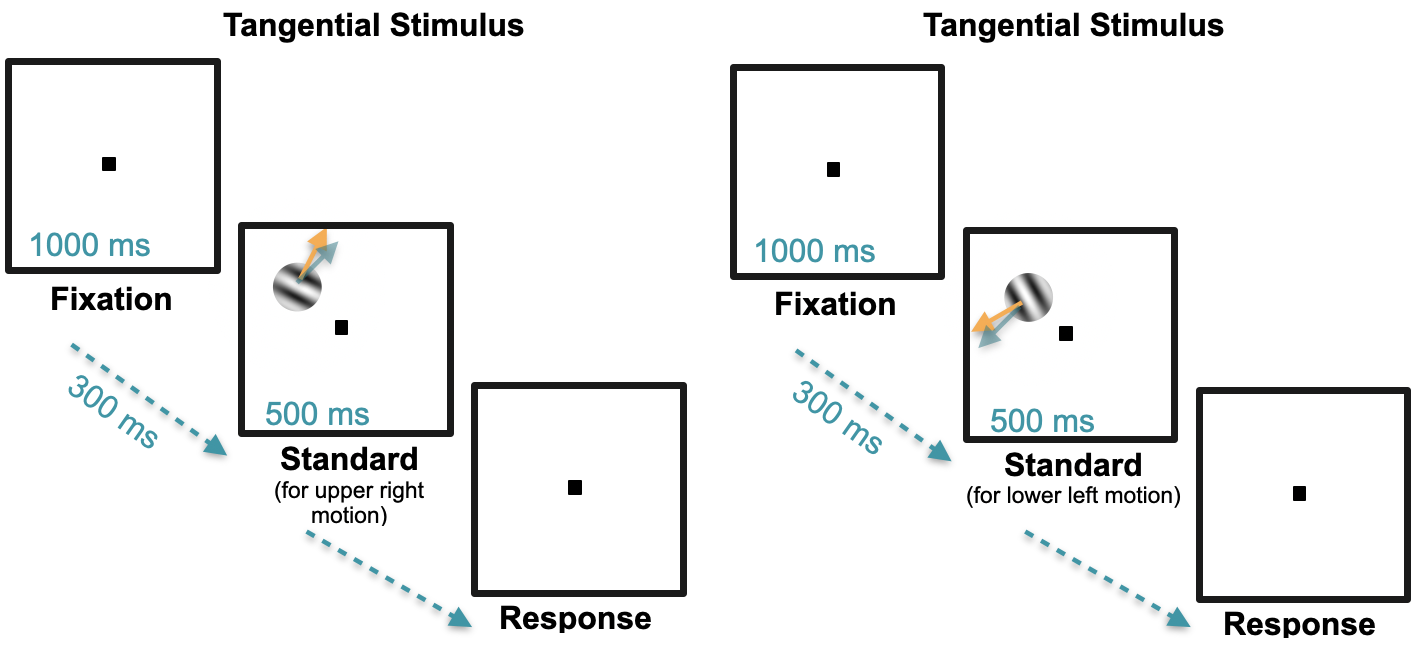
\includegraphics[scale=.4]{Images/Tang_sequence.png}
\caption{Blue arrow represents the internal reference, the orange arrow represents an example of the direction at which the stimulus is presented (can be clockwise or counterclockwise to the blue arrow.}
\end{figure}

\subsection{Block sequence}
Four blocks were run, and each block corresponded to 1 of the 4 conditions being tested (tangential lower left motion, tangential upper right motion, radial upper left motion, radial lower right motion). The internal reference frames for each block is shown below:

\begin{figure}[H]
\centering % centers the figure
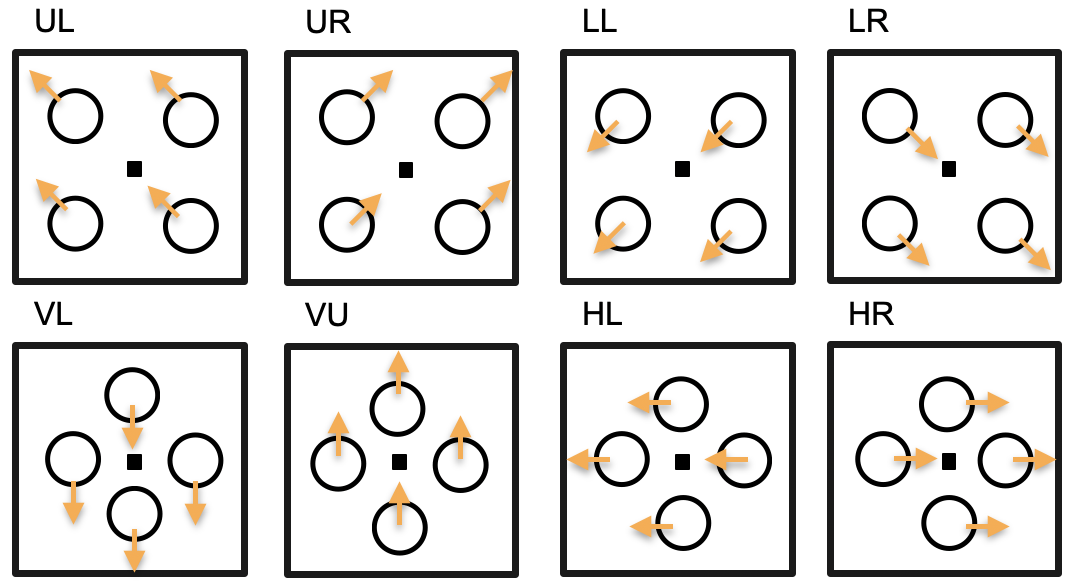
\includegraphics[scale=.4]{Images/Blocks.png}
\end{figure}

Prior to the actual experiment, the "standard" motion direction corresponding to that specific block will be showed to the observer to use as an internal reference. Then a training session is conducted to determine how much tilt is required to meet 75\% accuracy with staircase procedure (MLPest), and to allow subject to practice task with feedback. The estimated angular value to add/subtract to the standard to achieve 75\% performance of the clockwise/counterclockwise will be used to determine constants. For this pilot, constants [-8, -4, -2, -1, -0.5, 0.5, 1, 2, 4, 8] were chosen for all 8 blocks. Note positive and negative values for clockwise v. counterclockwise tilt.
\\
%Each block contains (2 locations with clockwise/counterclockwise motion) x 80 repetitions = 1,280 trials. All 4 full-blocks took 80 min. 
Each block contained 4 locations x 5 tilt values x 2 (clock v cc) x 20 repetitions = 800 trials. There are 8 blocks * 800 trials = 6400 total trials (3200 tang, 1600 radial-in, 1600 radial-out). Each full-block takes ~45 min; all 8 blocks took 360 min. 
\\
Example sequence of blocks for RE
\begin{enumerate}
\item diag-UL [angles: +- 0.5, 1, 2, 4, 8] (45 min)
\item card-HR [angles: +- 0.5, 1, 2, 4, 8] (45 min)
\item diag-LR [angles: +- 0.5, 1, 2, 4, 8] (45 min)
\item card-VL [angles: +- 0.5, 1, 2, 4, 8] (45 min)
\item diag-UR [angles: +- 0.5, 1, 2, 4, 8] (45 min)
\item card-HL [angles: +- 0.5, 1, 2, 4, 8] (45 min)
\item diag-LL [angles: +- 0.5, 1, 2, 4, 8] (45 min)
\item card-VU [angles: +- 0.5, 1, 2, 4, 8] (45 min)
\end{enumerate}

\newpage
\section{Subject Data (Relative motion)}
\subsection{Psychometric Fits}
\begin{figure}[H]
\centering % centers the figure
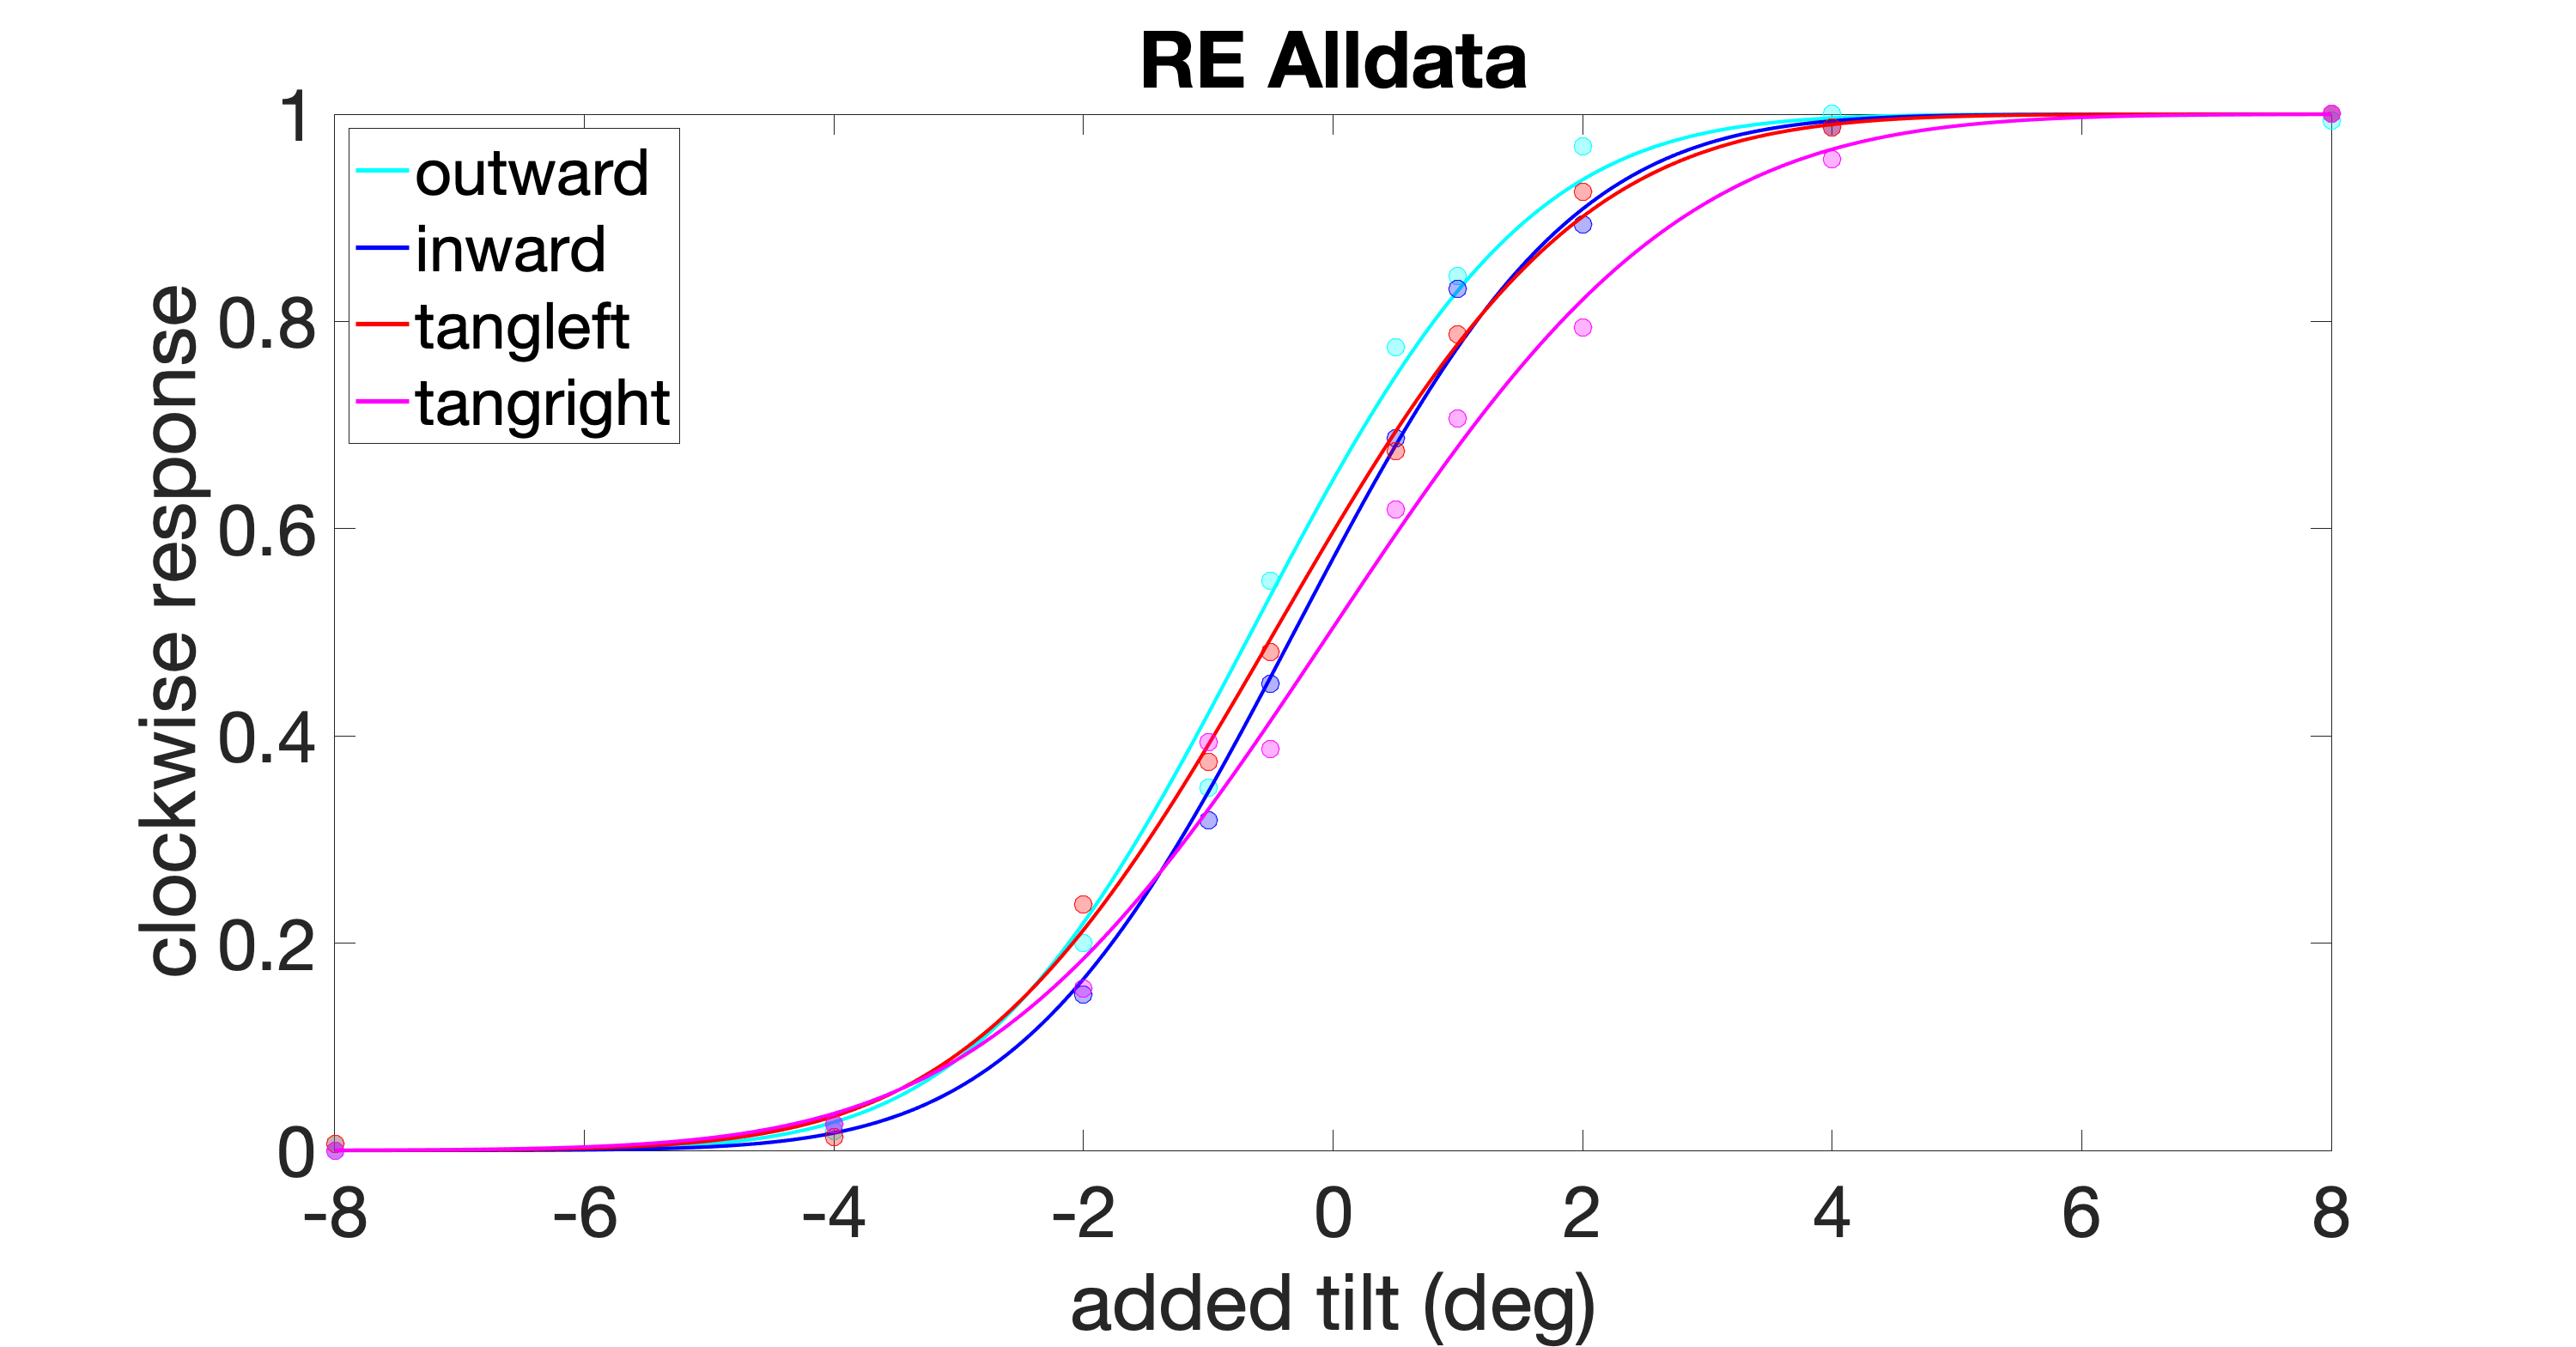
\includegraphics[scale=.16]{Images/RE_PF_Alldata_4conds.png}
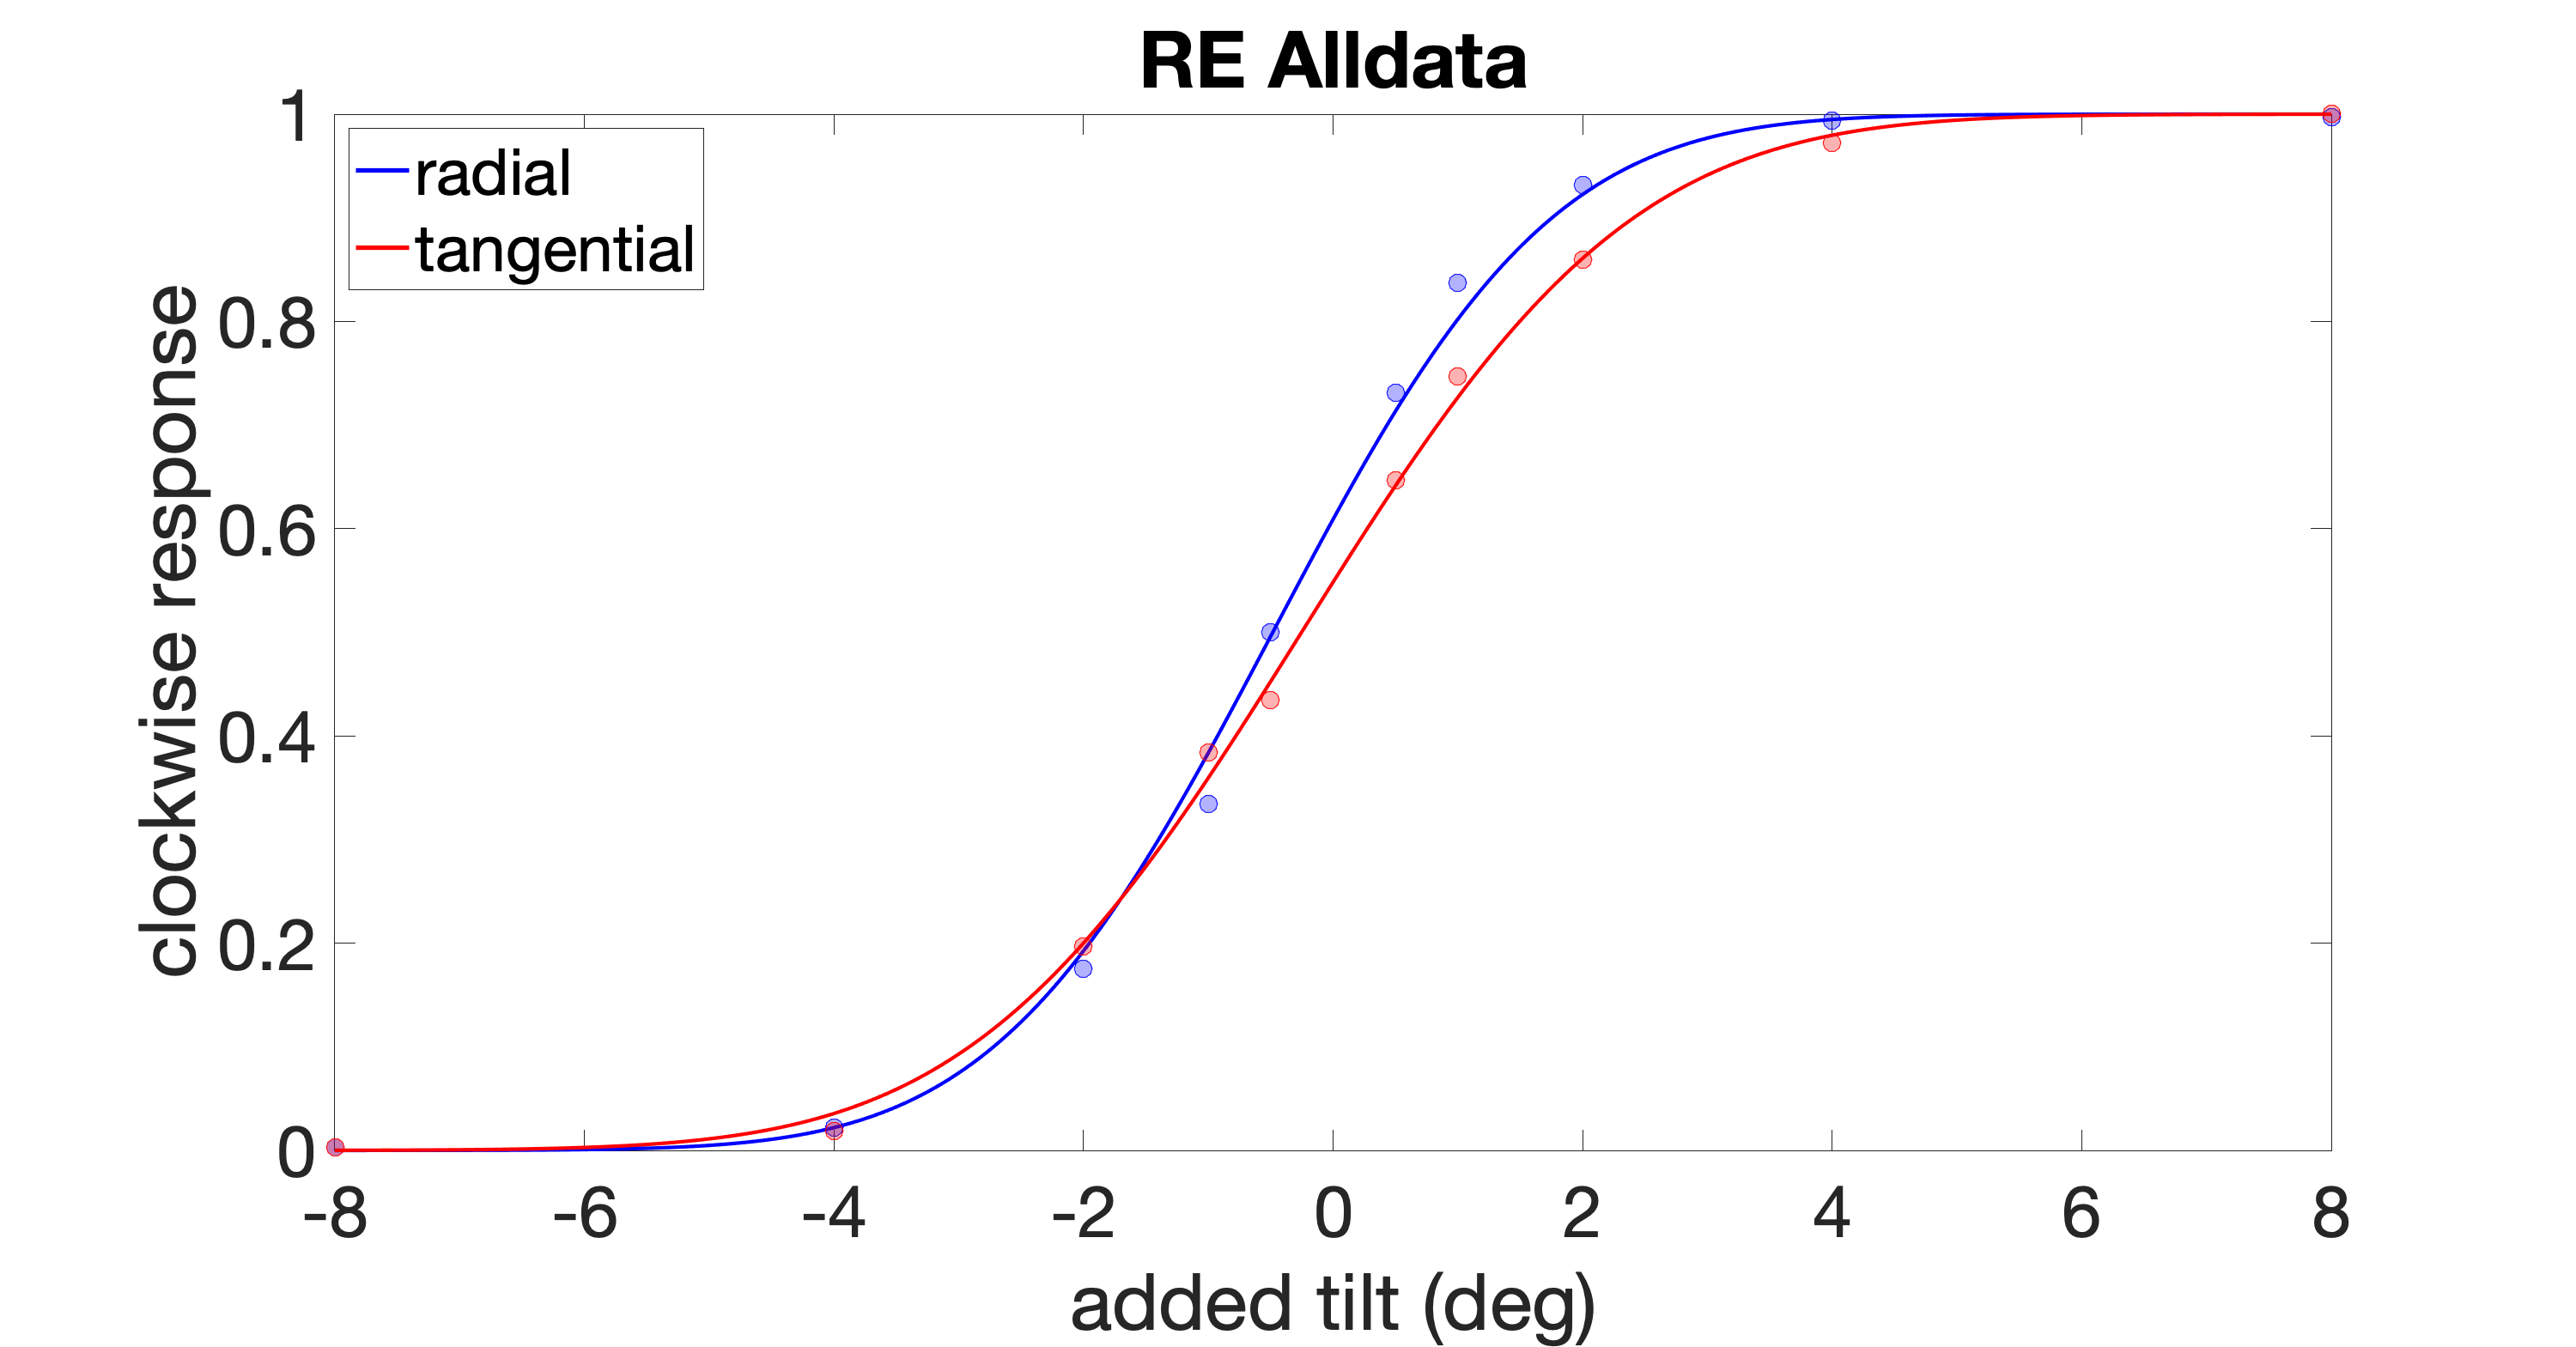
\includegraphics[scale=.16]{Images/RE_PF_Alldata_2conds.png}
\end{figure}
\begin{figure}[H]
\centering % centers the figure
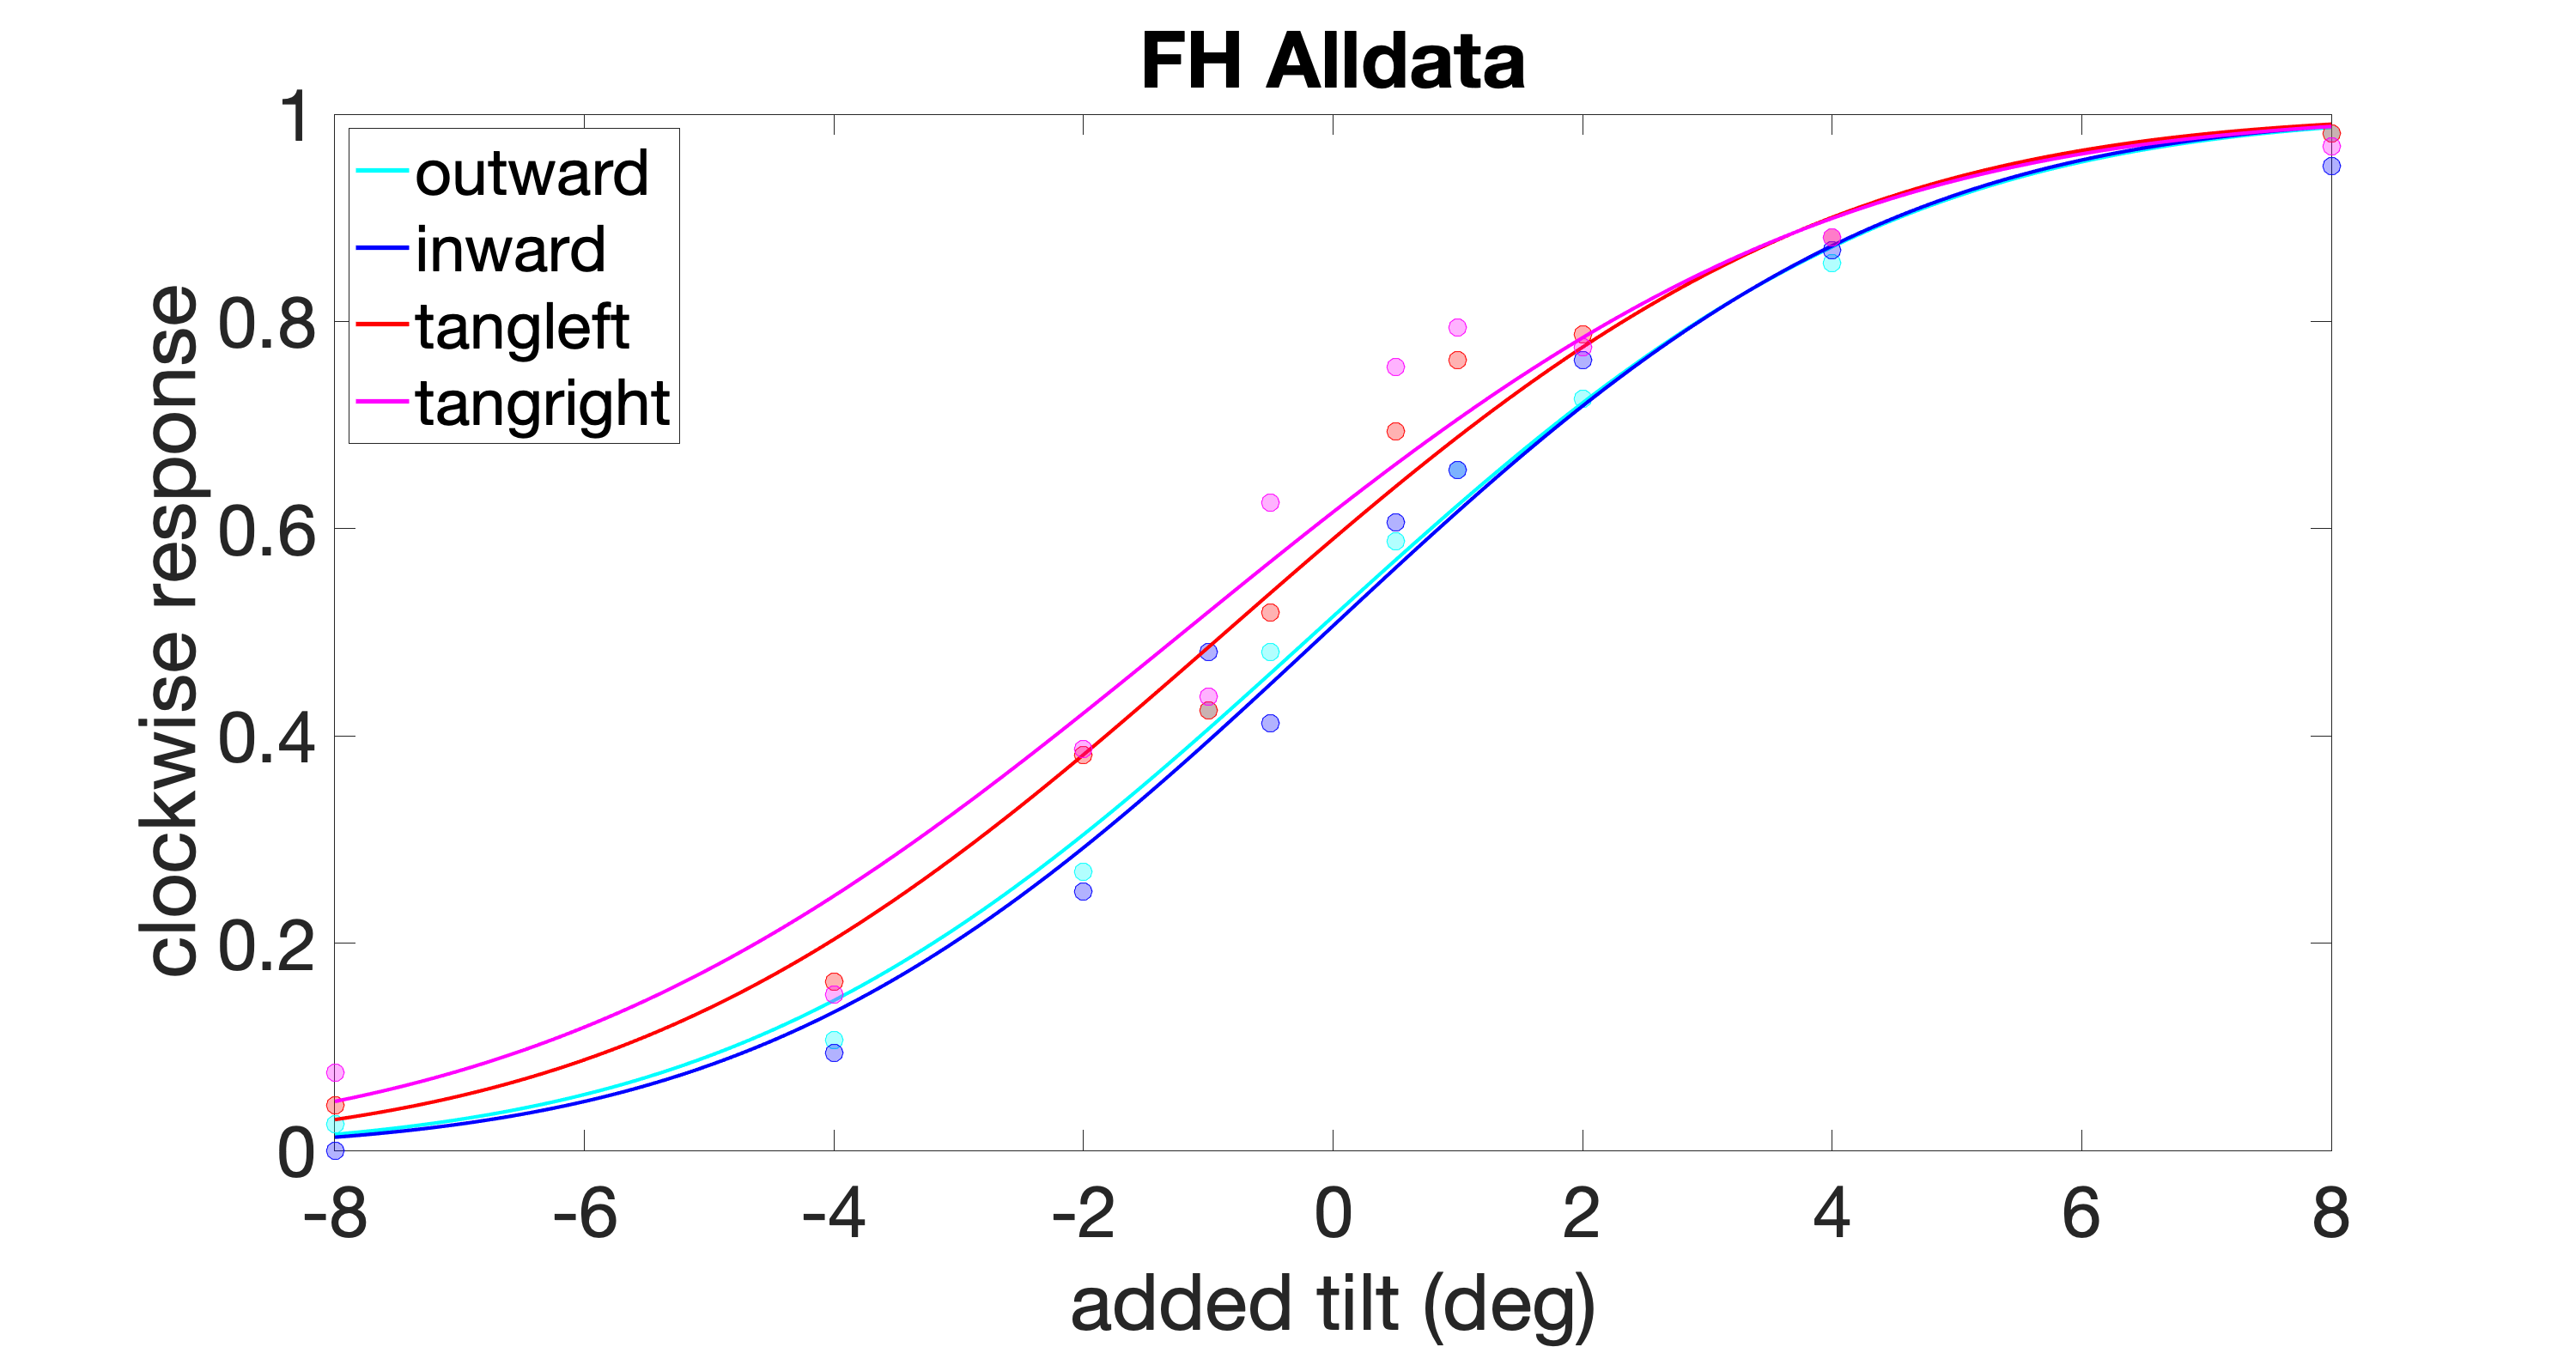
\includegraphics[scale=.16]{Images/FH_PF_Alldata_4conds.png}
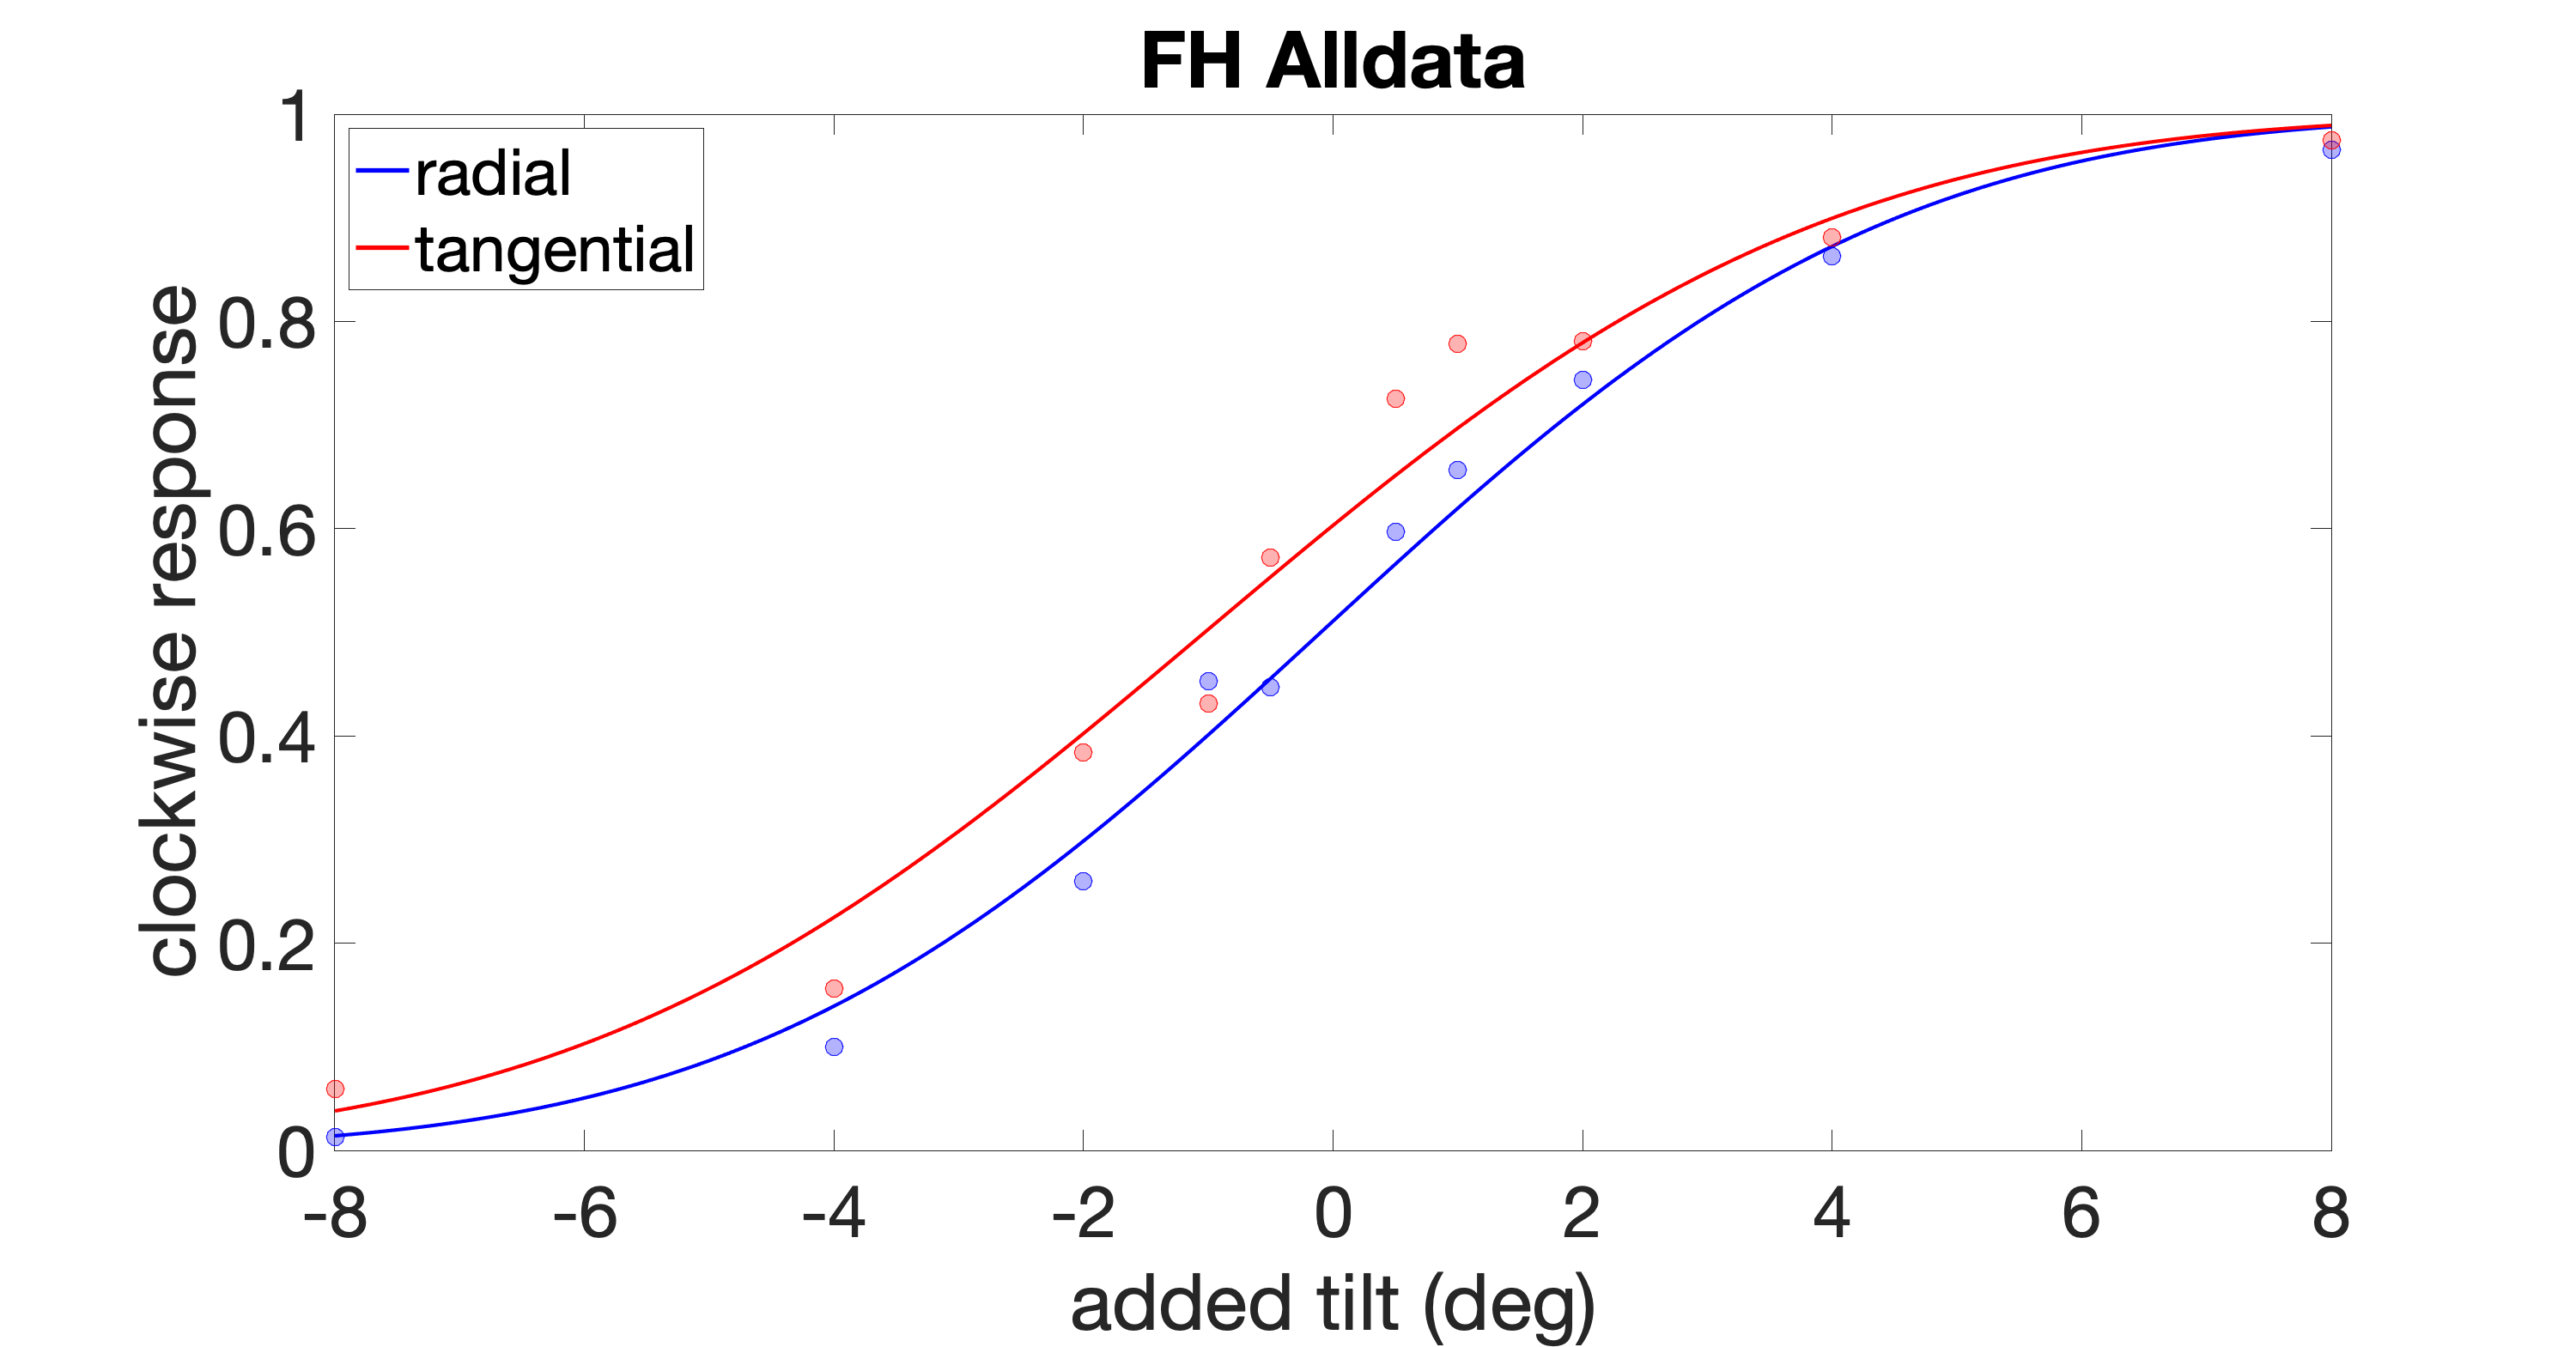
\includegraphics[scale=.16]{Images/FH_PF_Alldata_2conds.png}
\end{figure}
\begin{figure}[H]
\centering % centers the figure
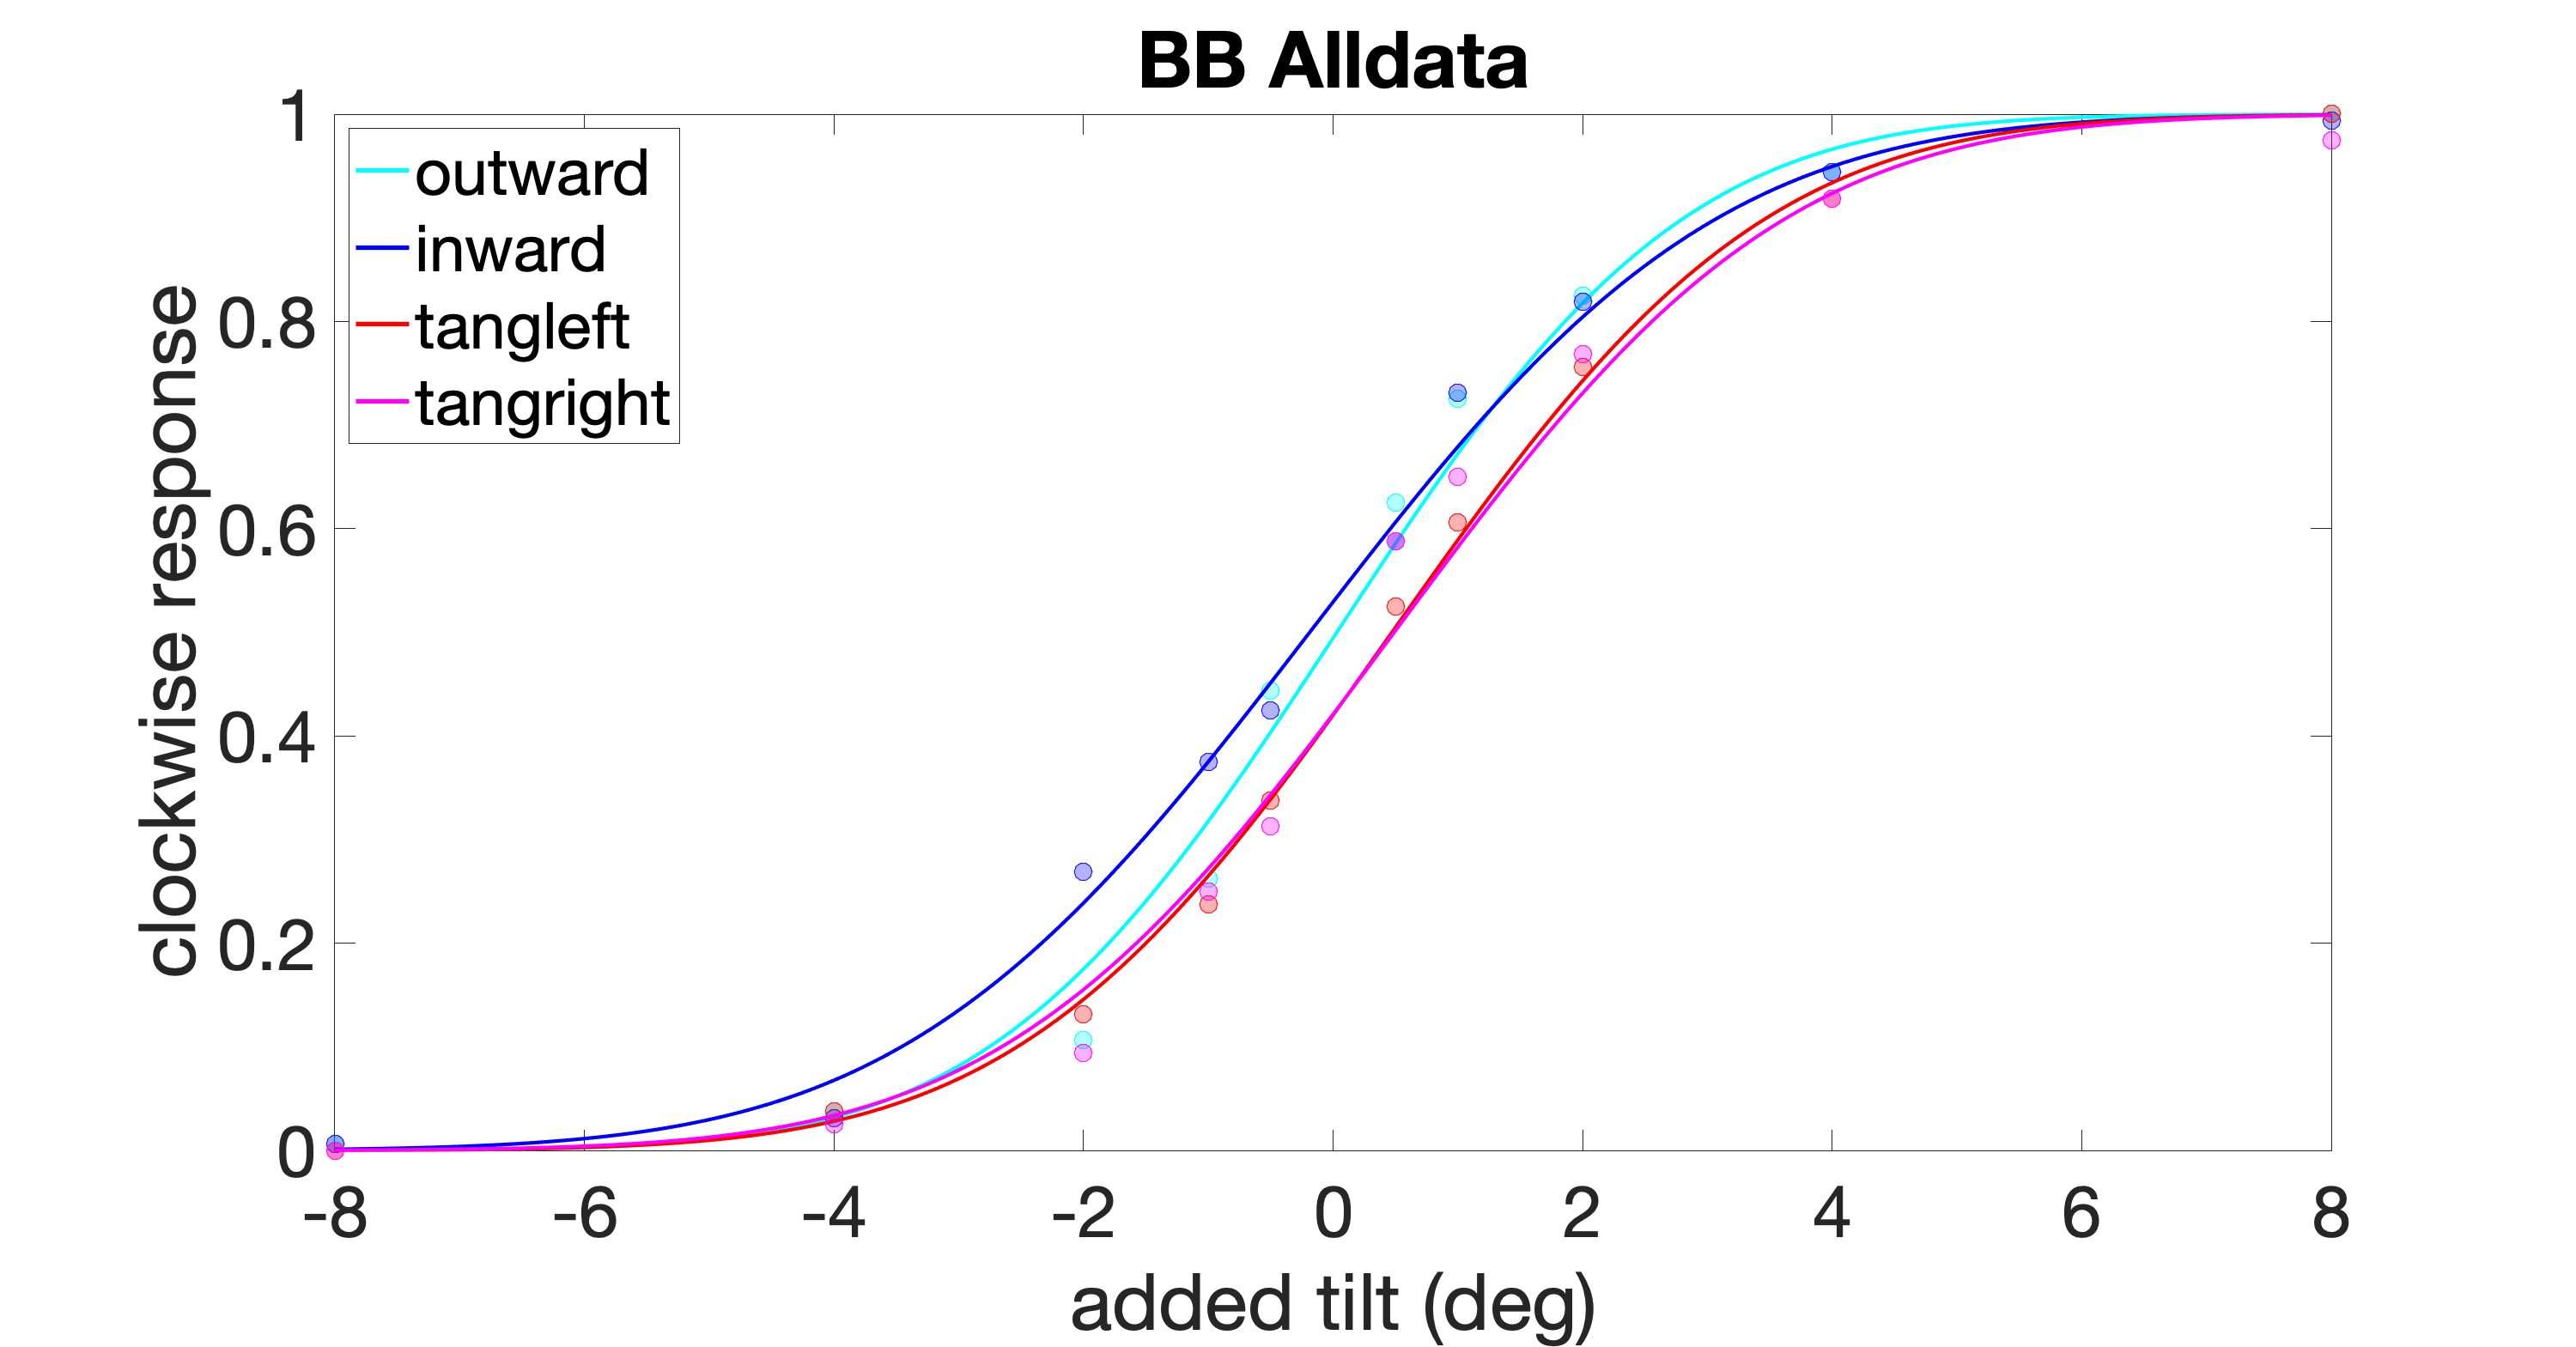
\includegraphics[scale=.16]{Images/BB_PF_Alldata_4conds.png}
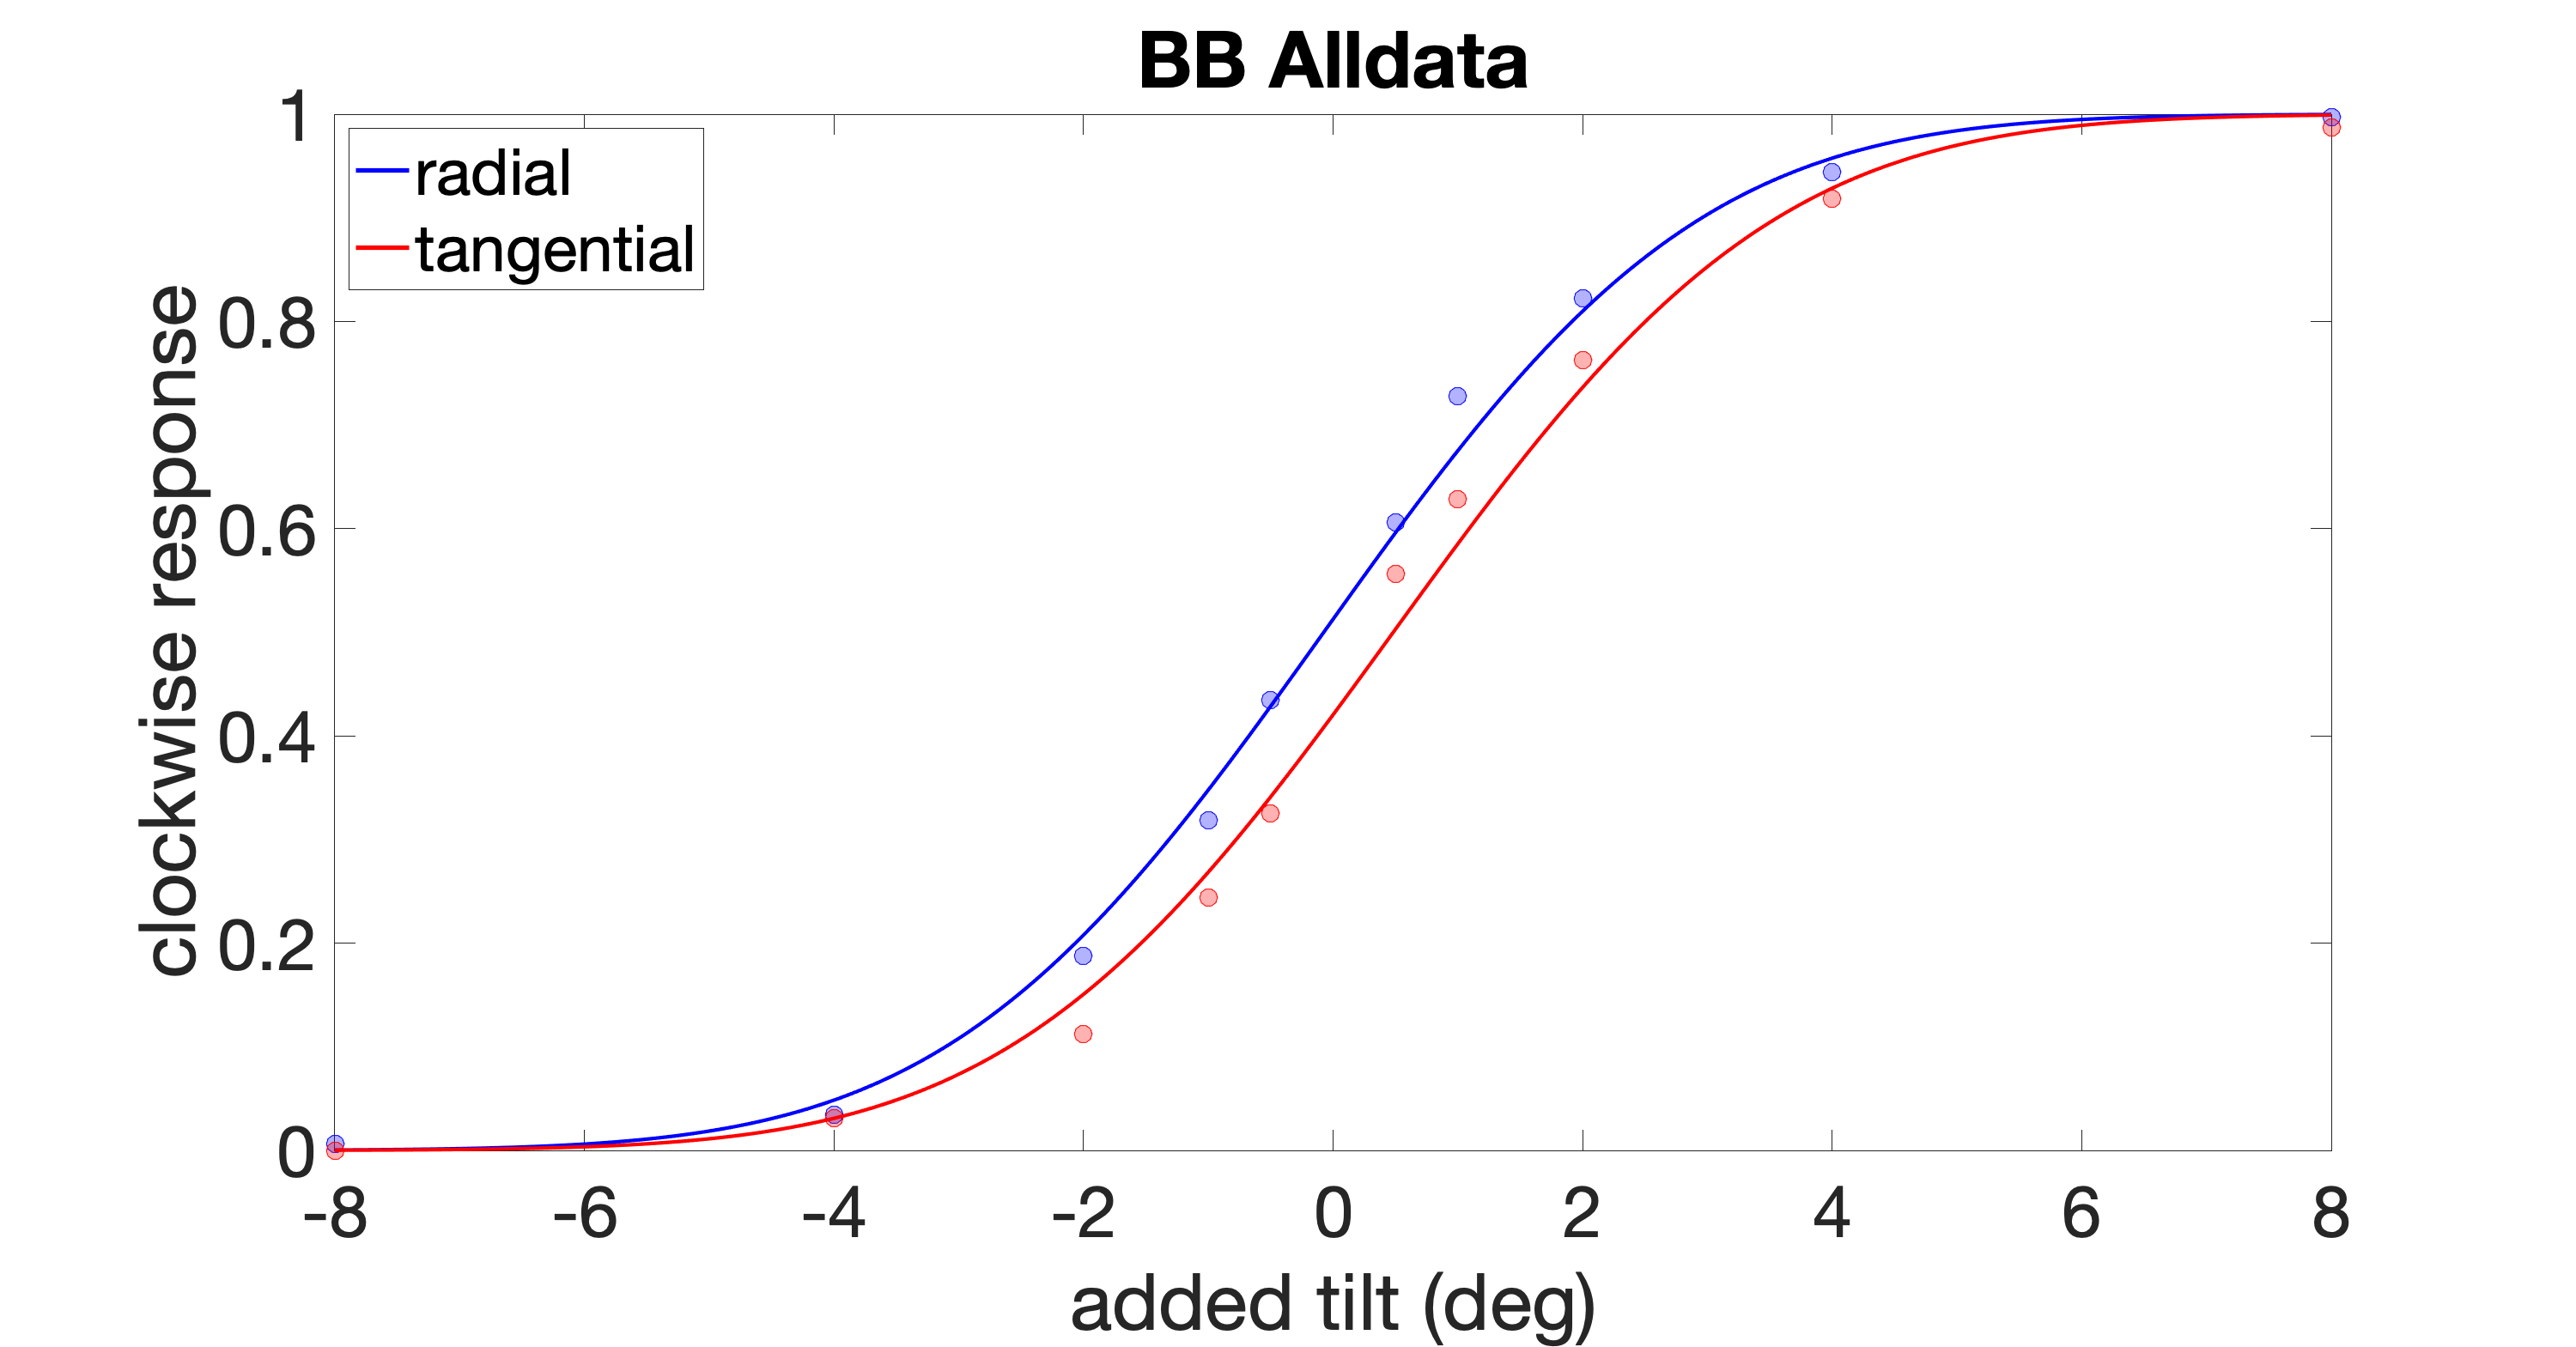
\includegraphics[scale=.16]{Images/BB_PF_Alldata_2conds.png}
\end{figure}
\begin{figure}[H]
\centering % centers the figure
\includegraphics[scale=.16]{Images/PW_PF_Alldata_4conds.png}
\includegraphics[scale=.16]{Images/PW_PF_Alldata_2conds.png}
\end{figure}
\begin{figure}[H]
\centering % centers the figure
\includegraphics[scale=.16]{Images/NH_PF_Alldata_4conds.png}
\includegraphics[scale=.16]{Images/NH_PF_Alldata_2conds.png}
\caption{LEFT: 200 trials per point. RIGHT: Each point is 400 trials.}
\end{figure}

\newpage
\subsection{Sensitivity Polar Plots: Relative Motion}
\begin{figure}[H]
\centering % centers the figure
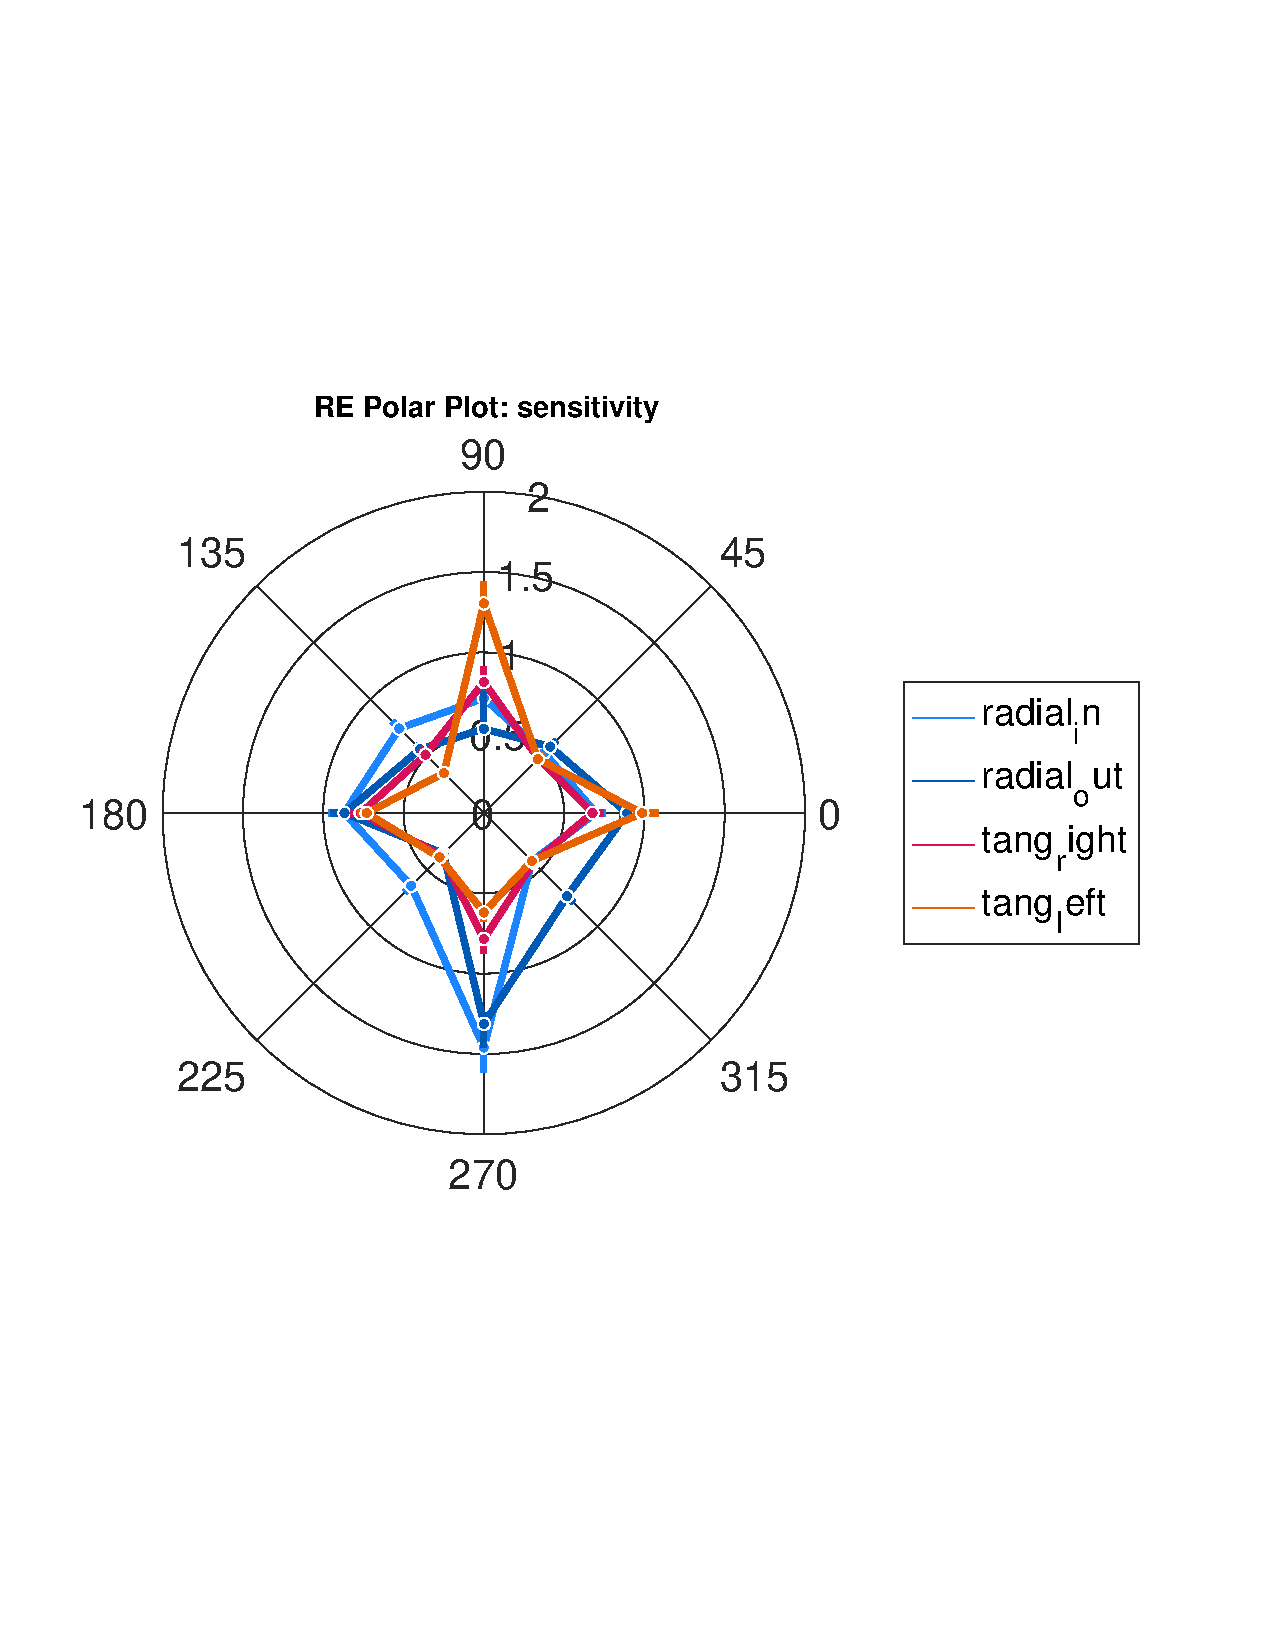
\includegraphics[scale=.3]{Images/RE_PP_sensitivity_Alldata_4conds_relative.png}
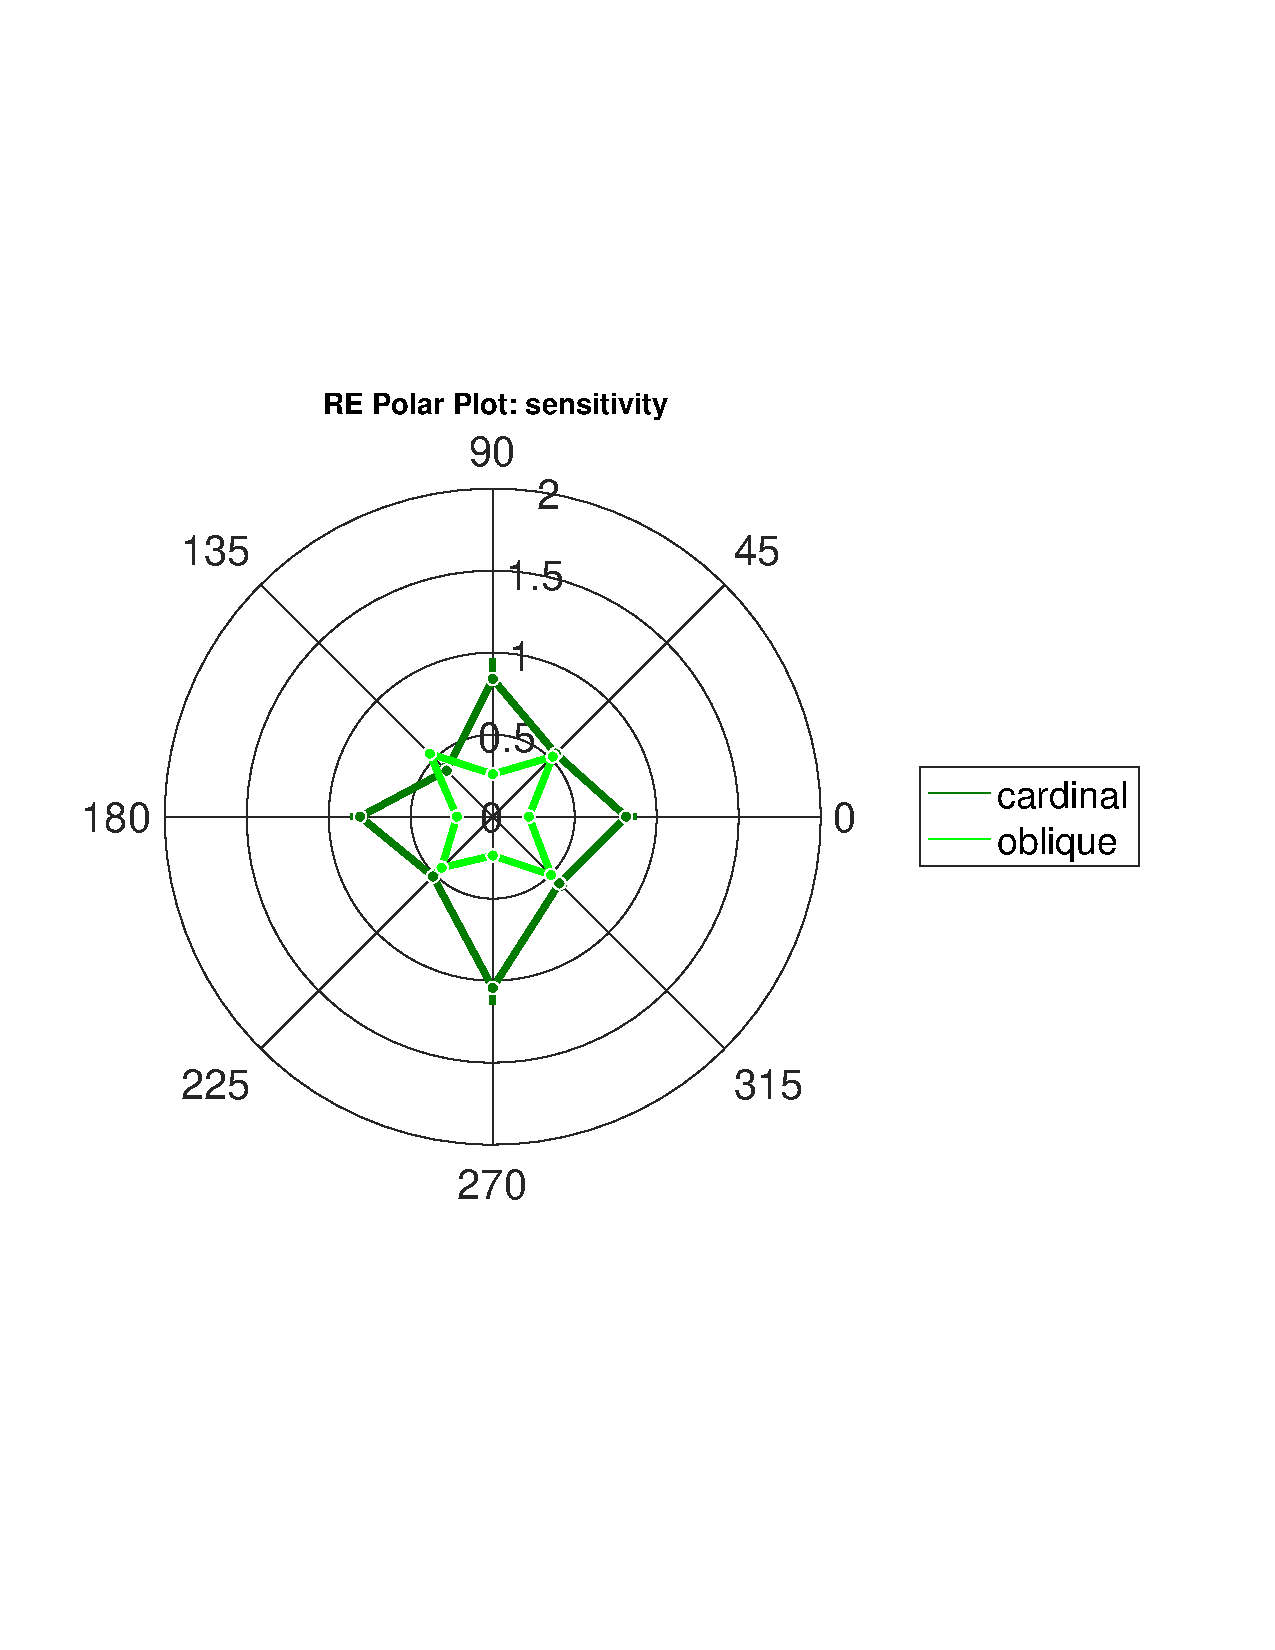
\includegraphics[scale=.3]{Images/RE_PP_sensitivity_Alldata_2conds_relative.png}
\end{figure}
\begin{figure}[H]
\centering % centers the figure
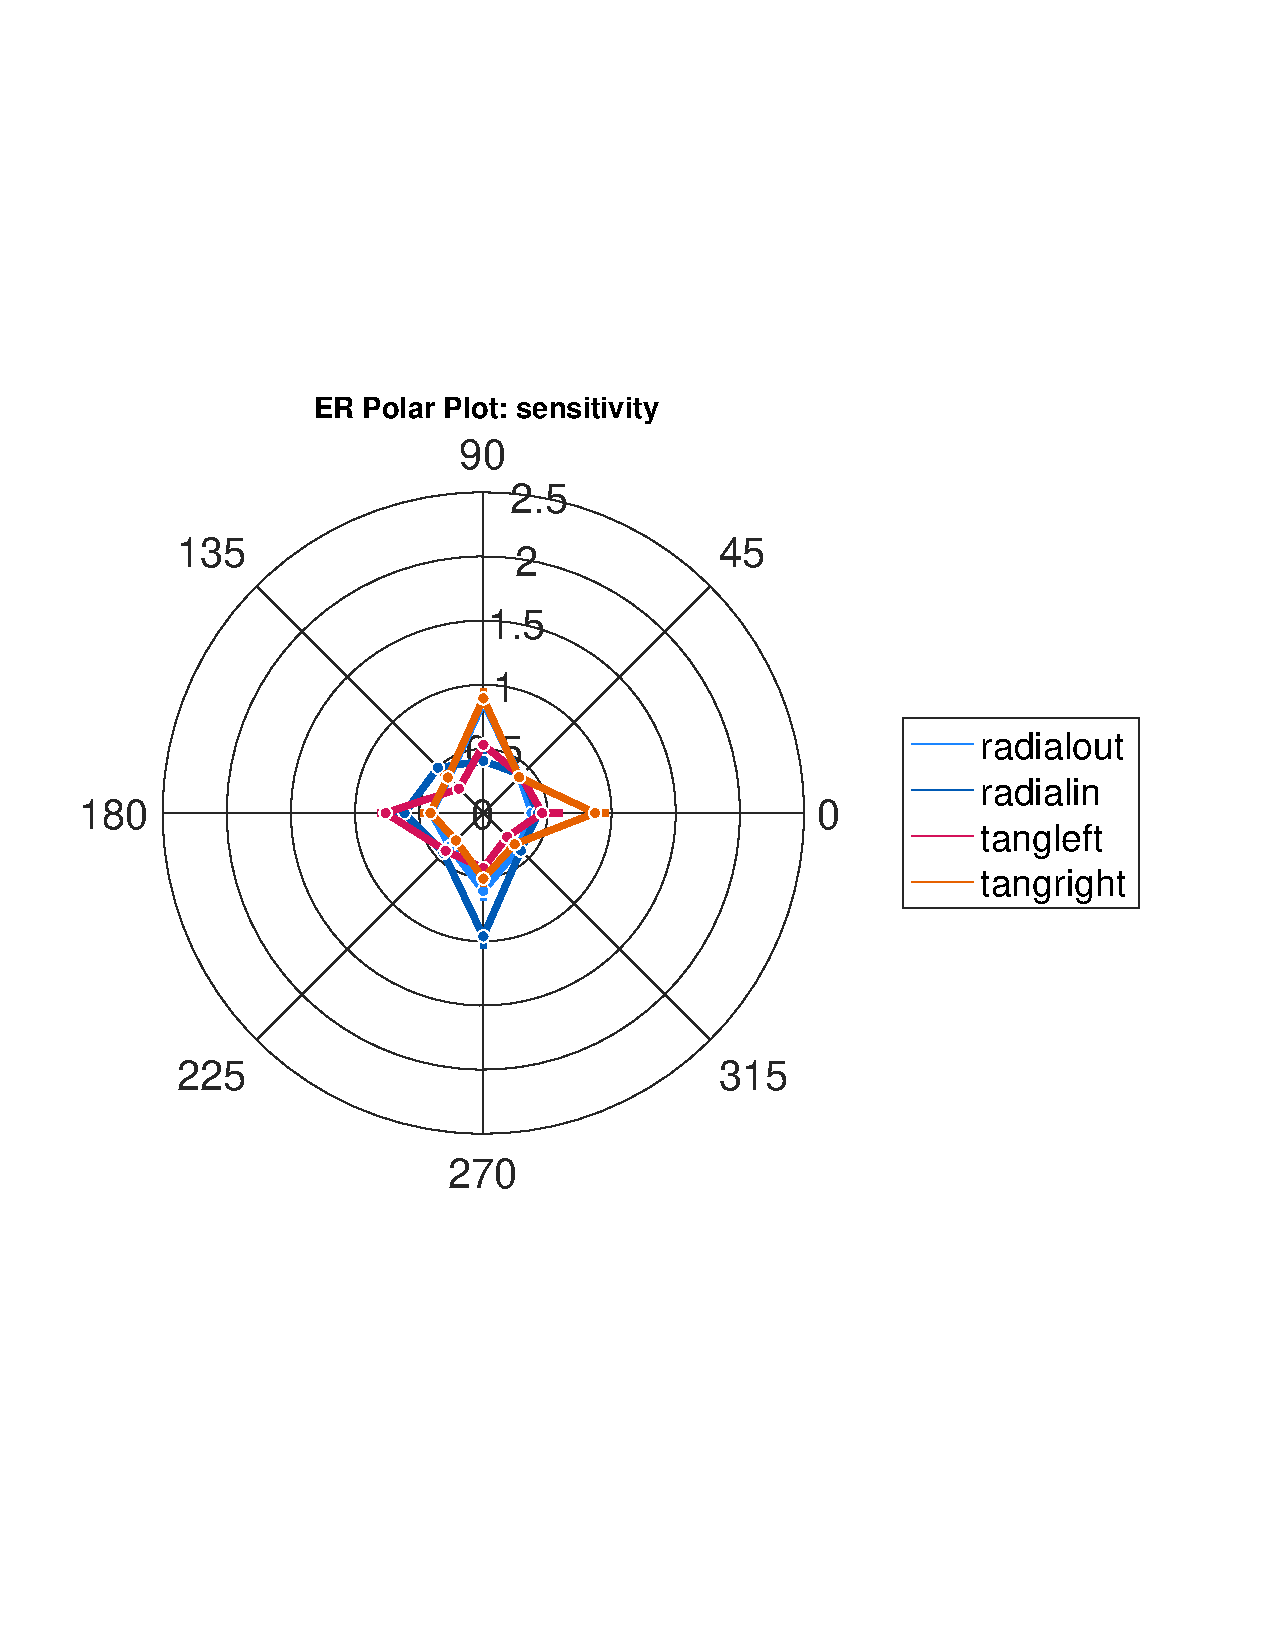
\includegraphics[scale=.3]{Images/ER_PP_sensitivity_Alldata_4conds_relative.png}
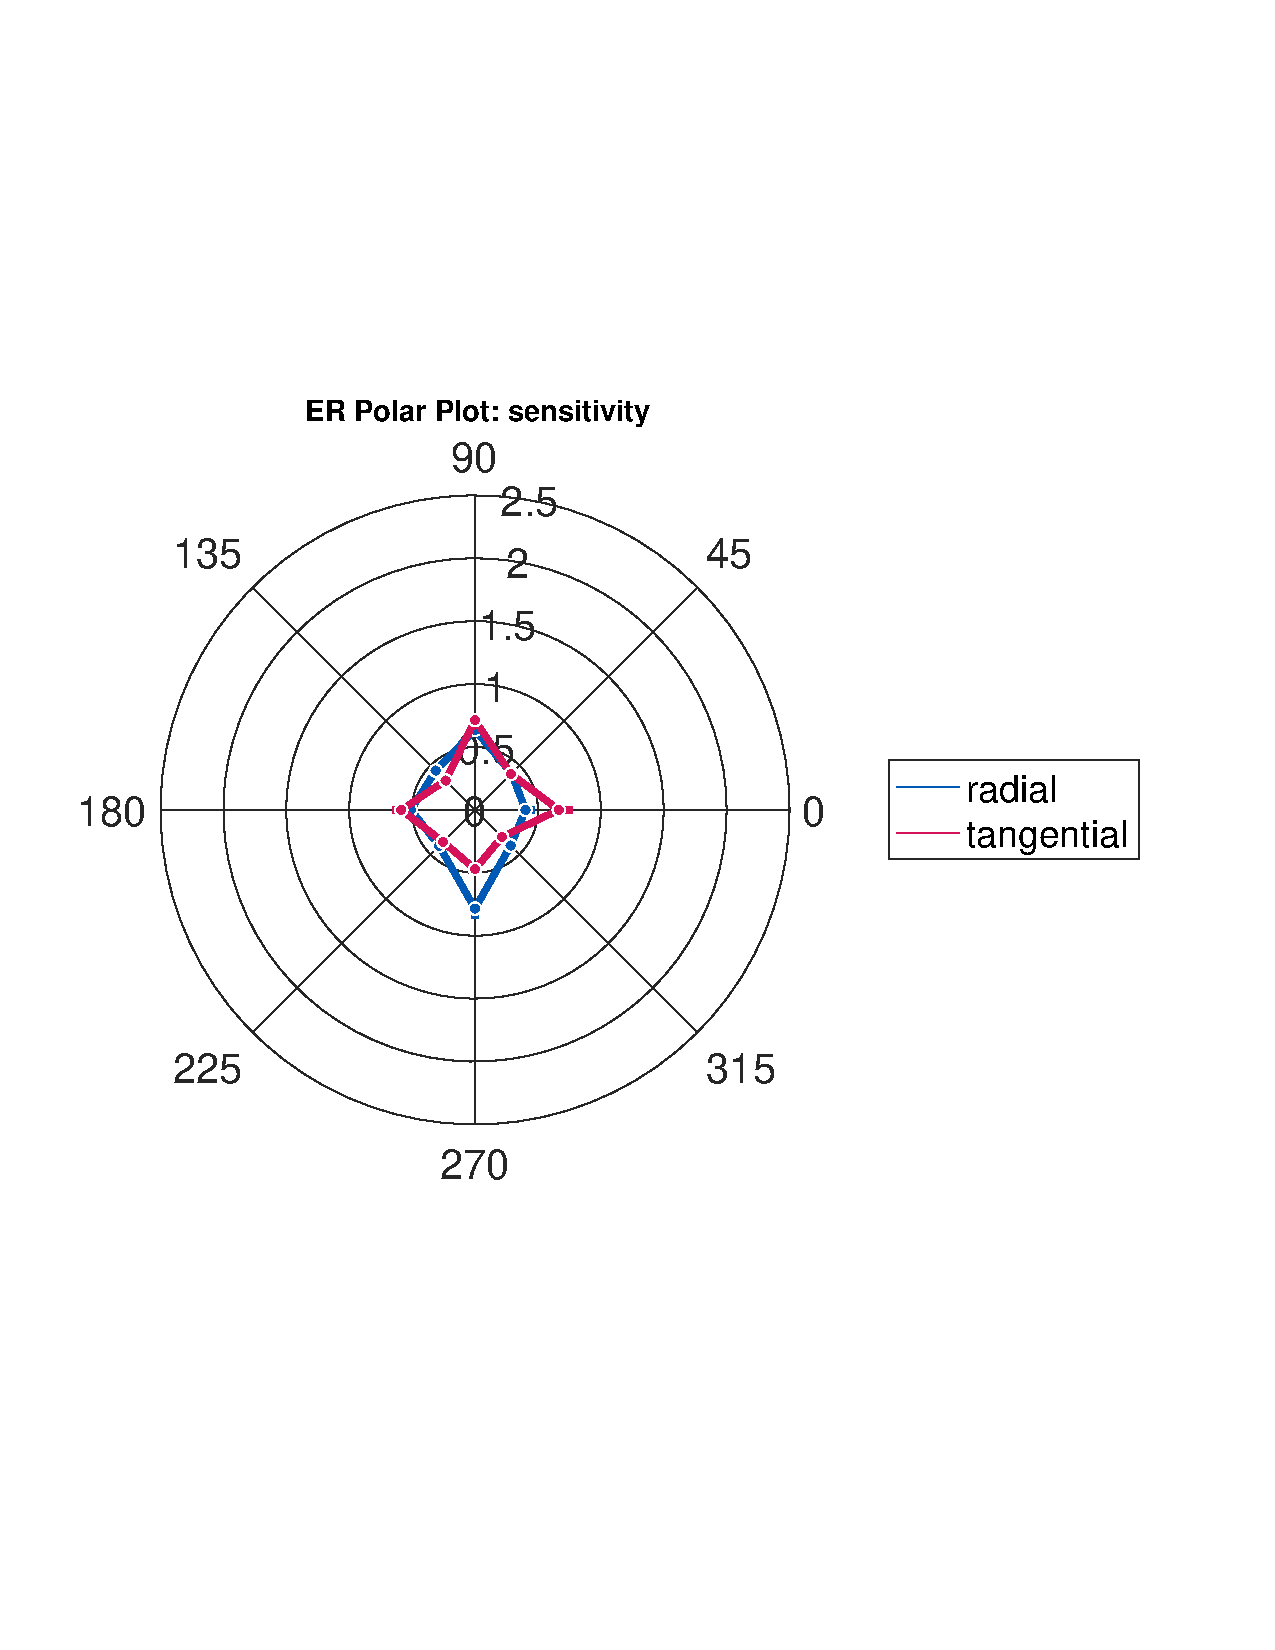
\includegraphics[scale=.3]{Images/ER_PP_sensitivity_Alldata_2conds_relative.png}
\caption{Same subject (RE) but at half distance.}
\end{figure}
\begin{figure}[H]
\centering % centers the figure
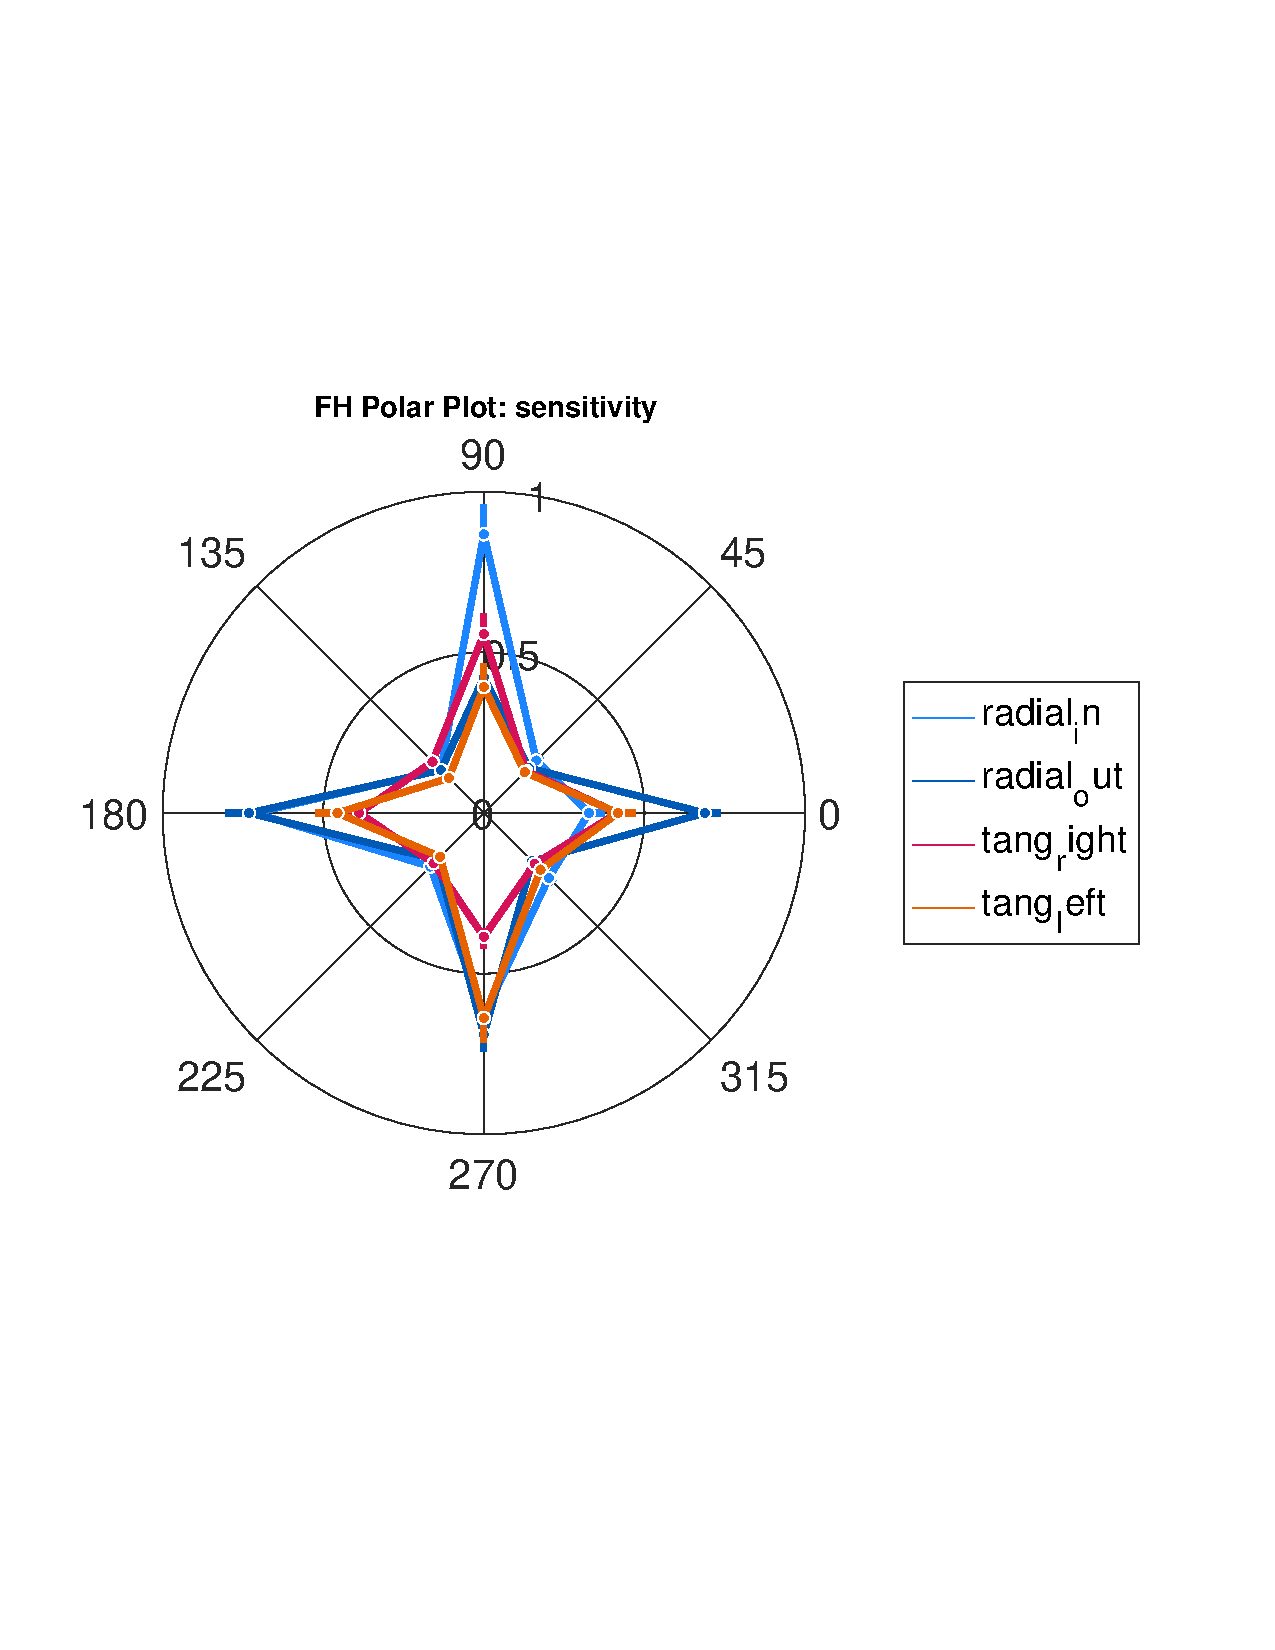
\includegraphics[scale=.3]{Images/FH_PP_sensitivity_Alldata_4conds_relative.png}
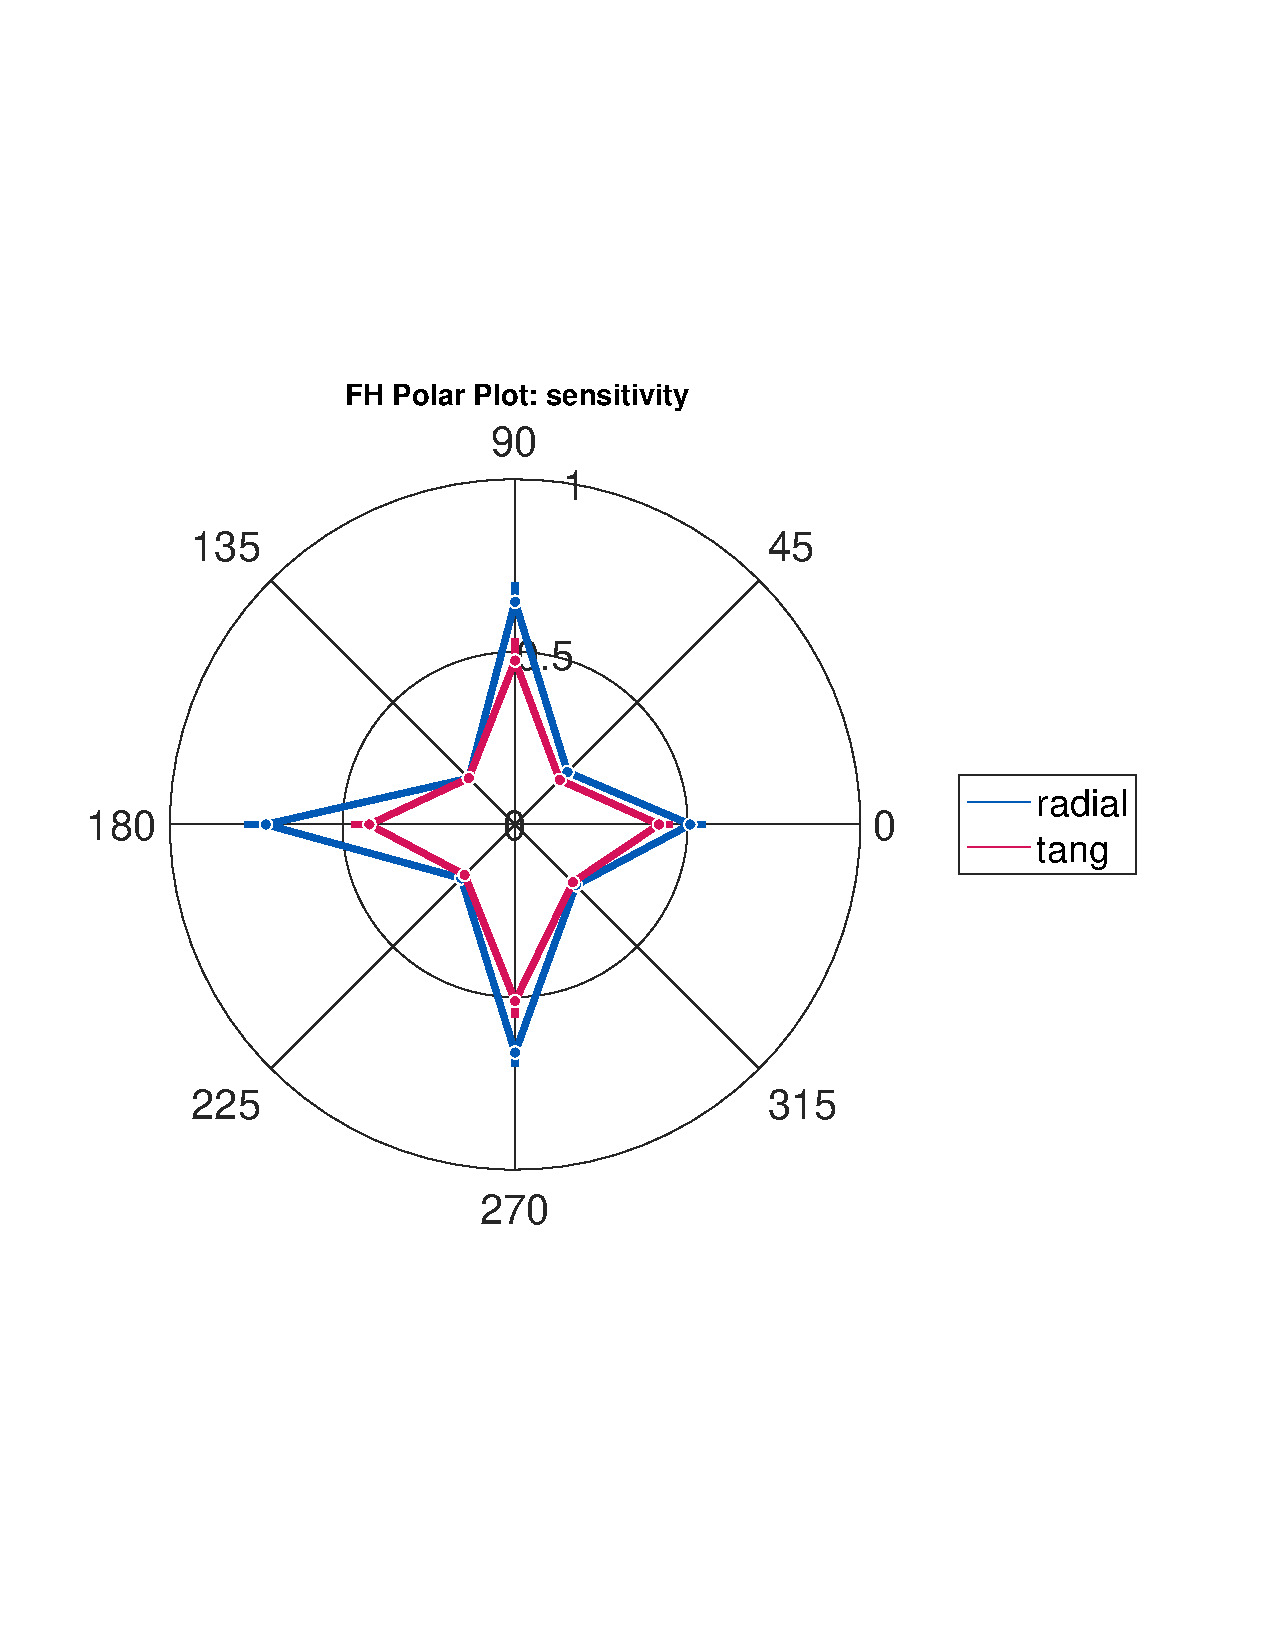
\includegraphics[scale=.3]{Images/FH_PP_sensitivity_Alldata_2conds_relative.png}
\end{figure}
\begin{figure}[H]
\centering % centers the figure
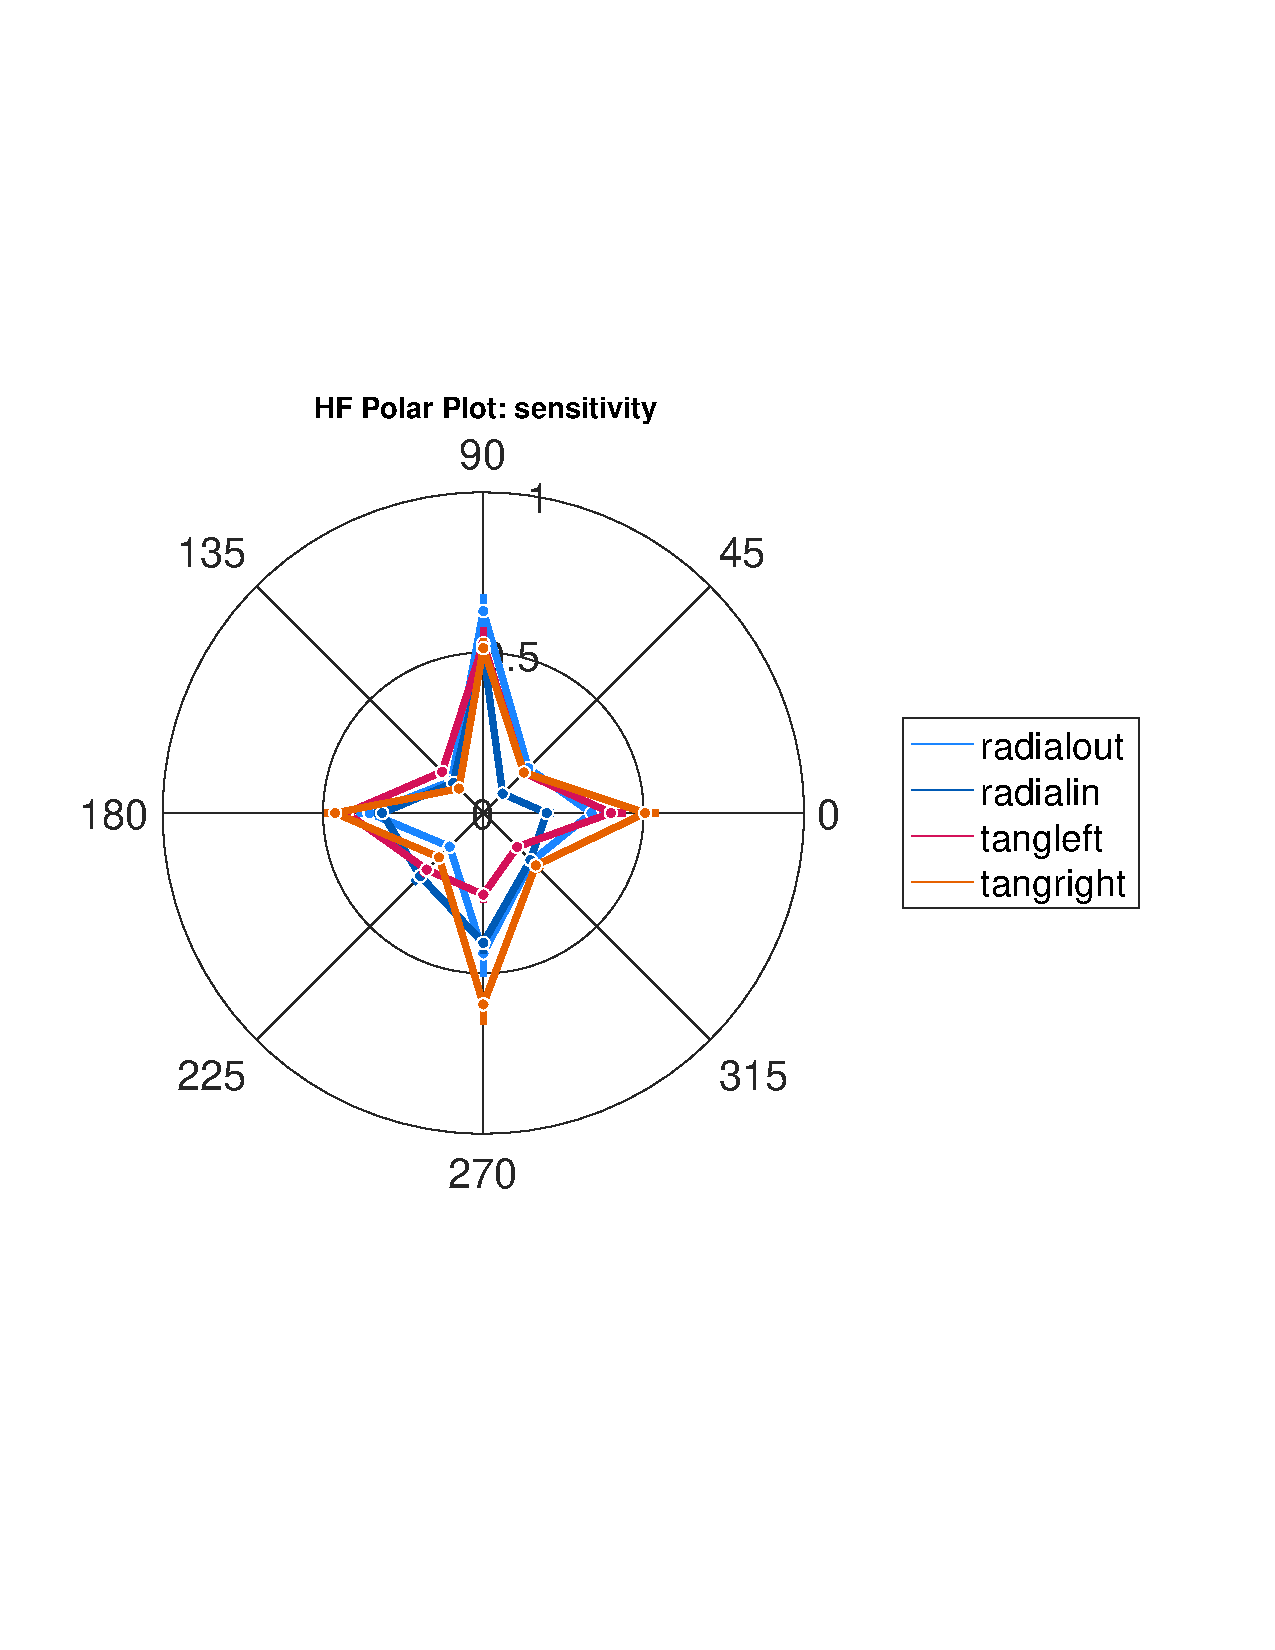
\includegraphics[scale=.3]{Images/HF_PP_sensitivity_Alldata_4conds_relative.png}
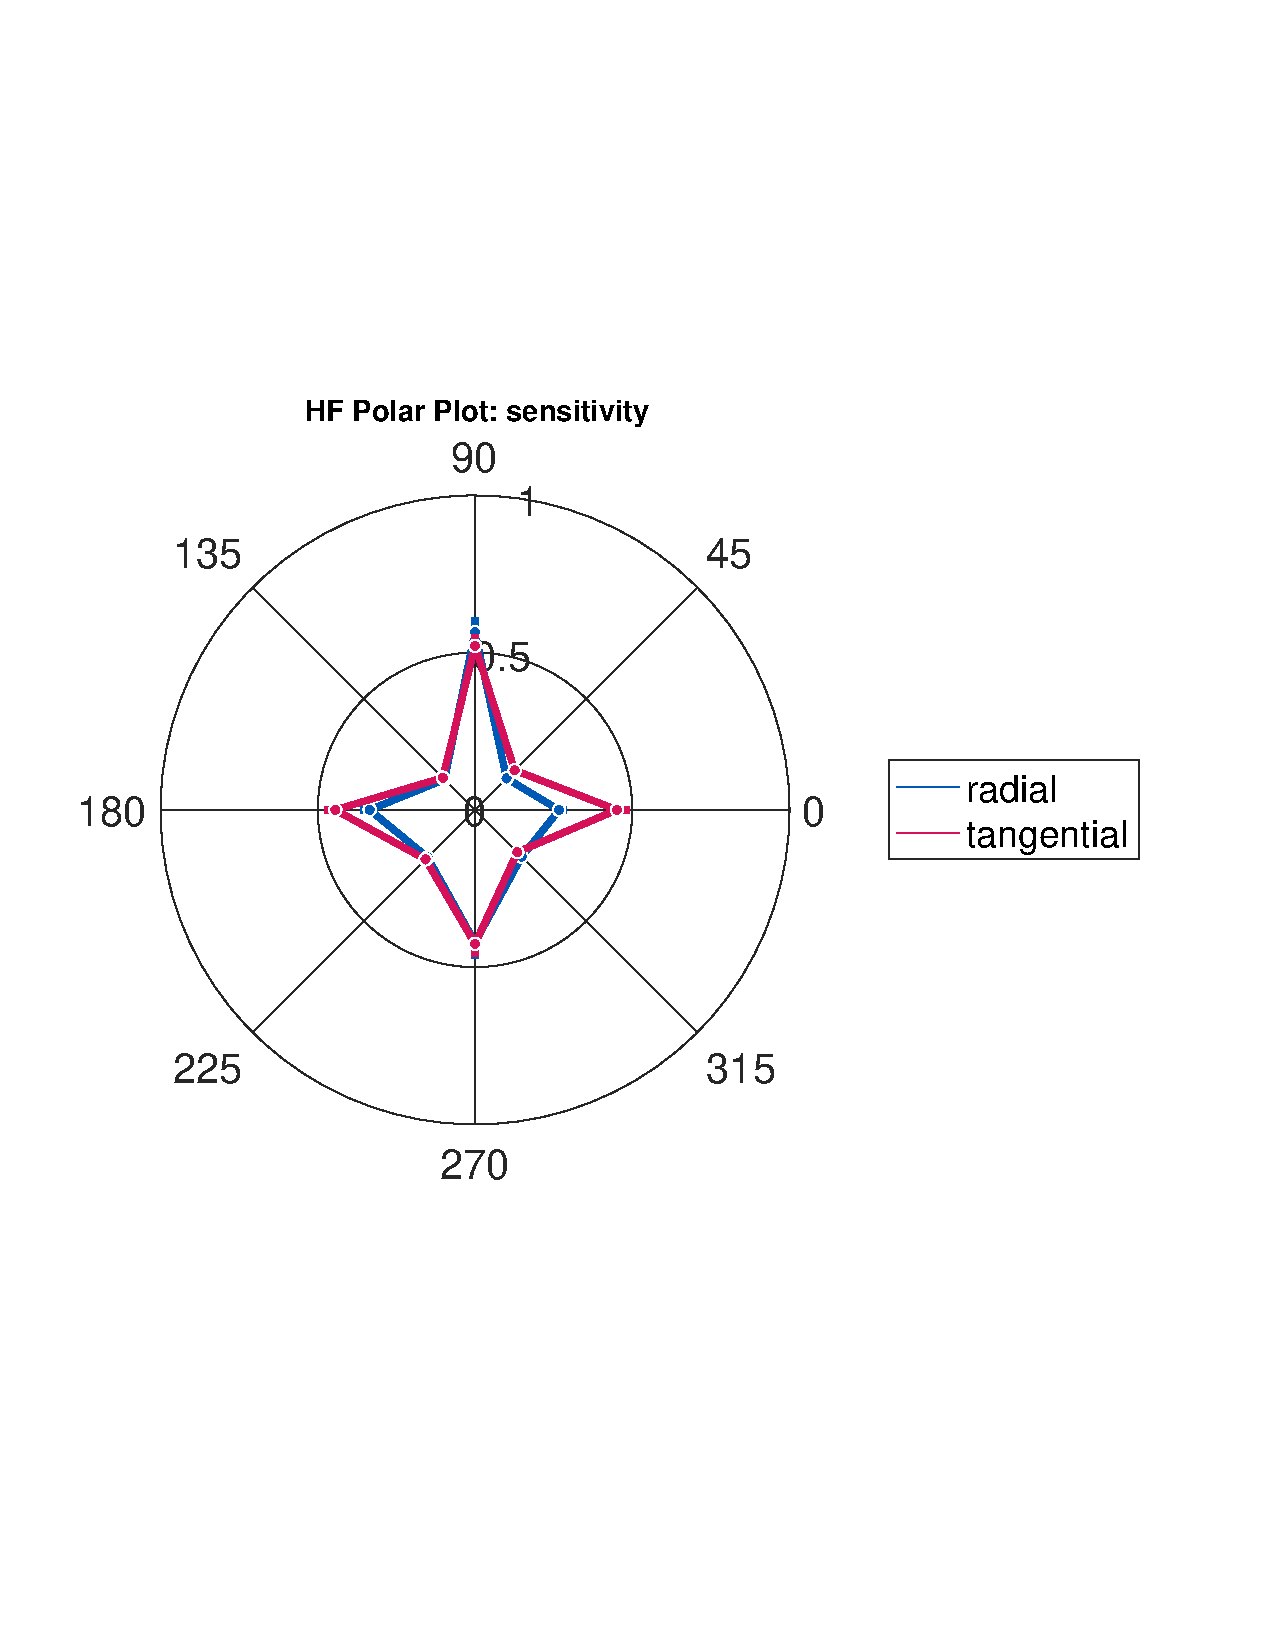
\includegraphics[scale=.3]{Images/HF_PP_sensitivity_Alldata_2conds_relative.png}
\caption{Same subject (FH) but at half distance.}
\end{figure}
\begin{figure}[H]
\centering % centers the figure
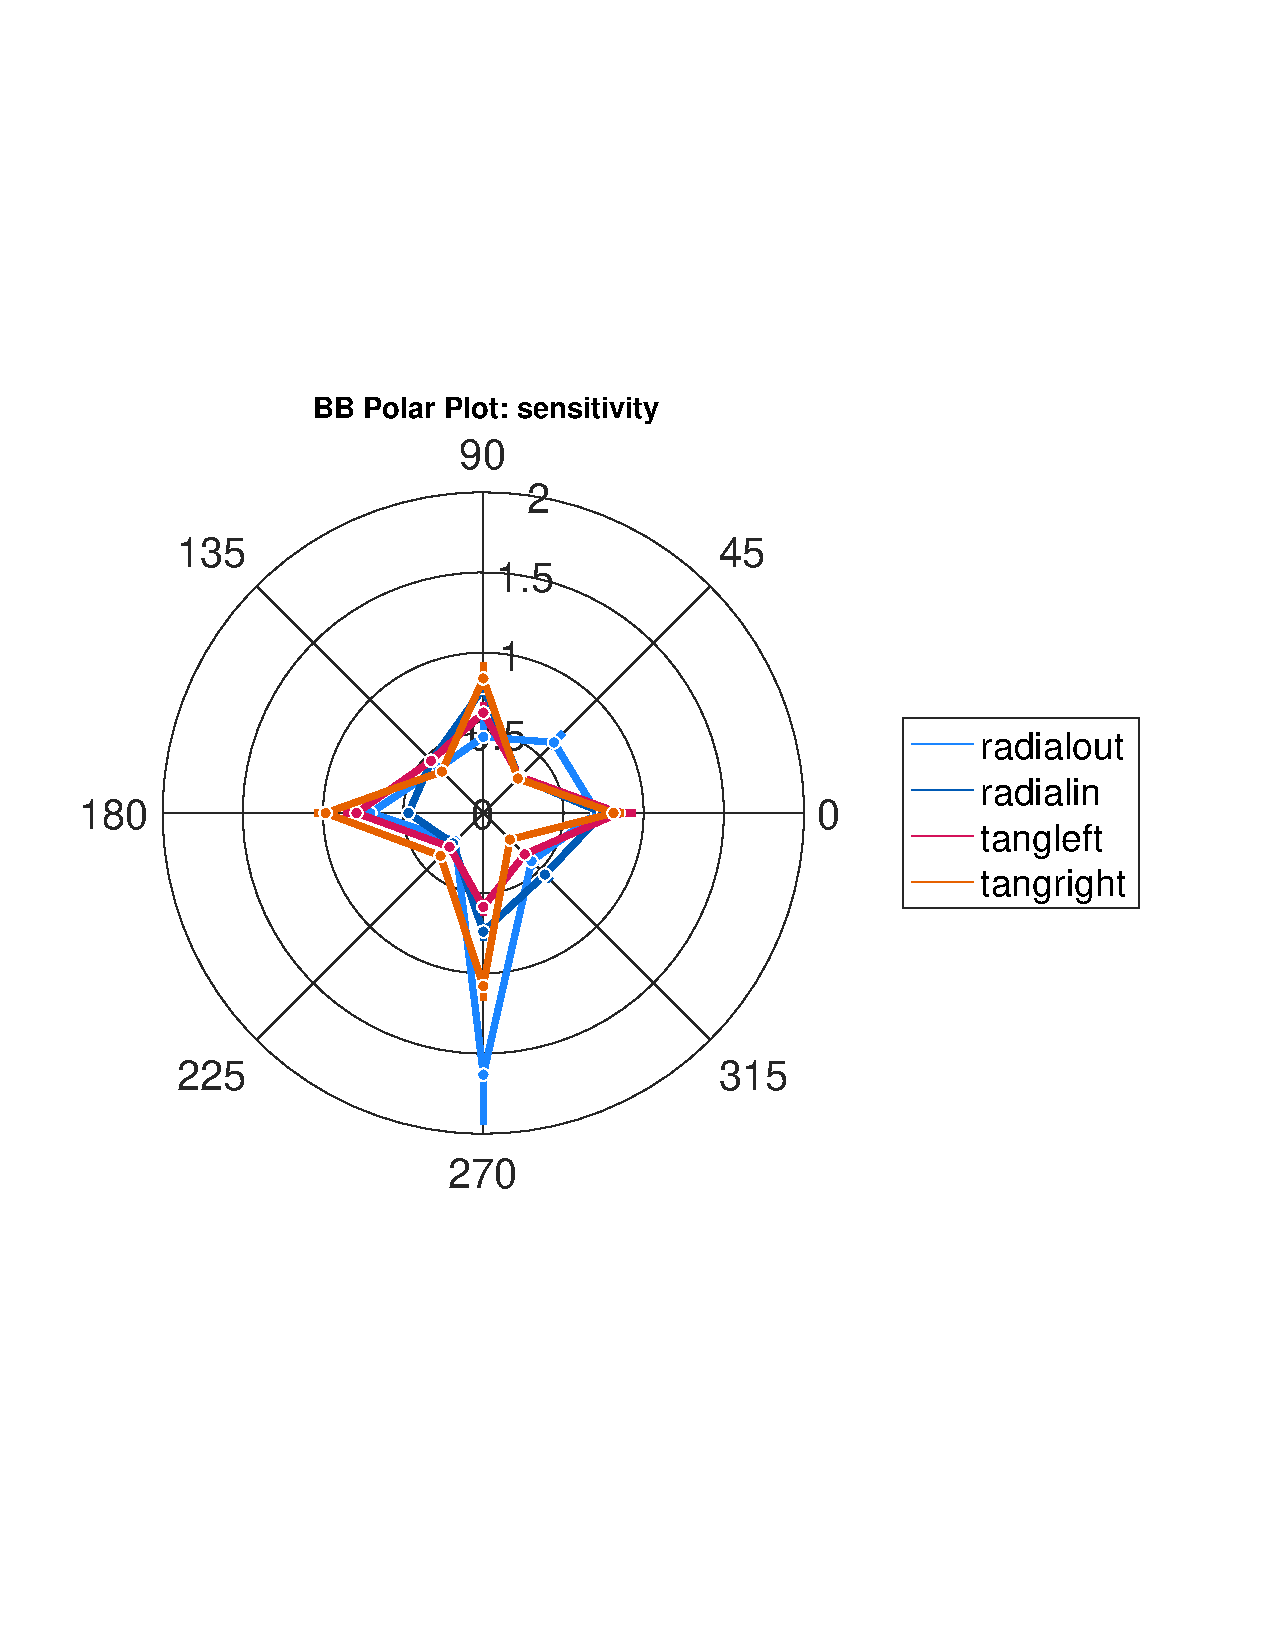
\includegraphics[scale=.3]{Images/BB_PP_sensitivity_Alldata_4conds_relative.png}
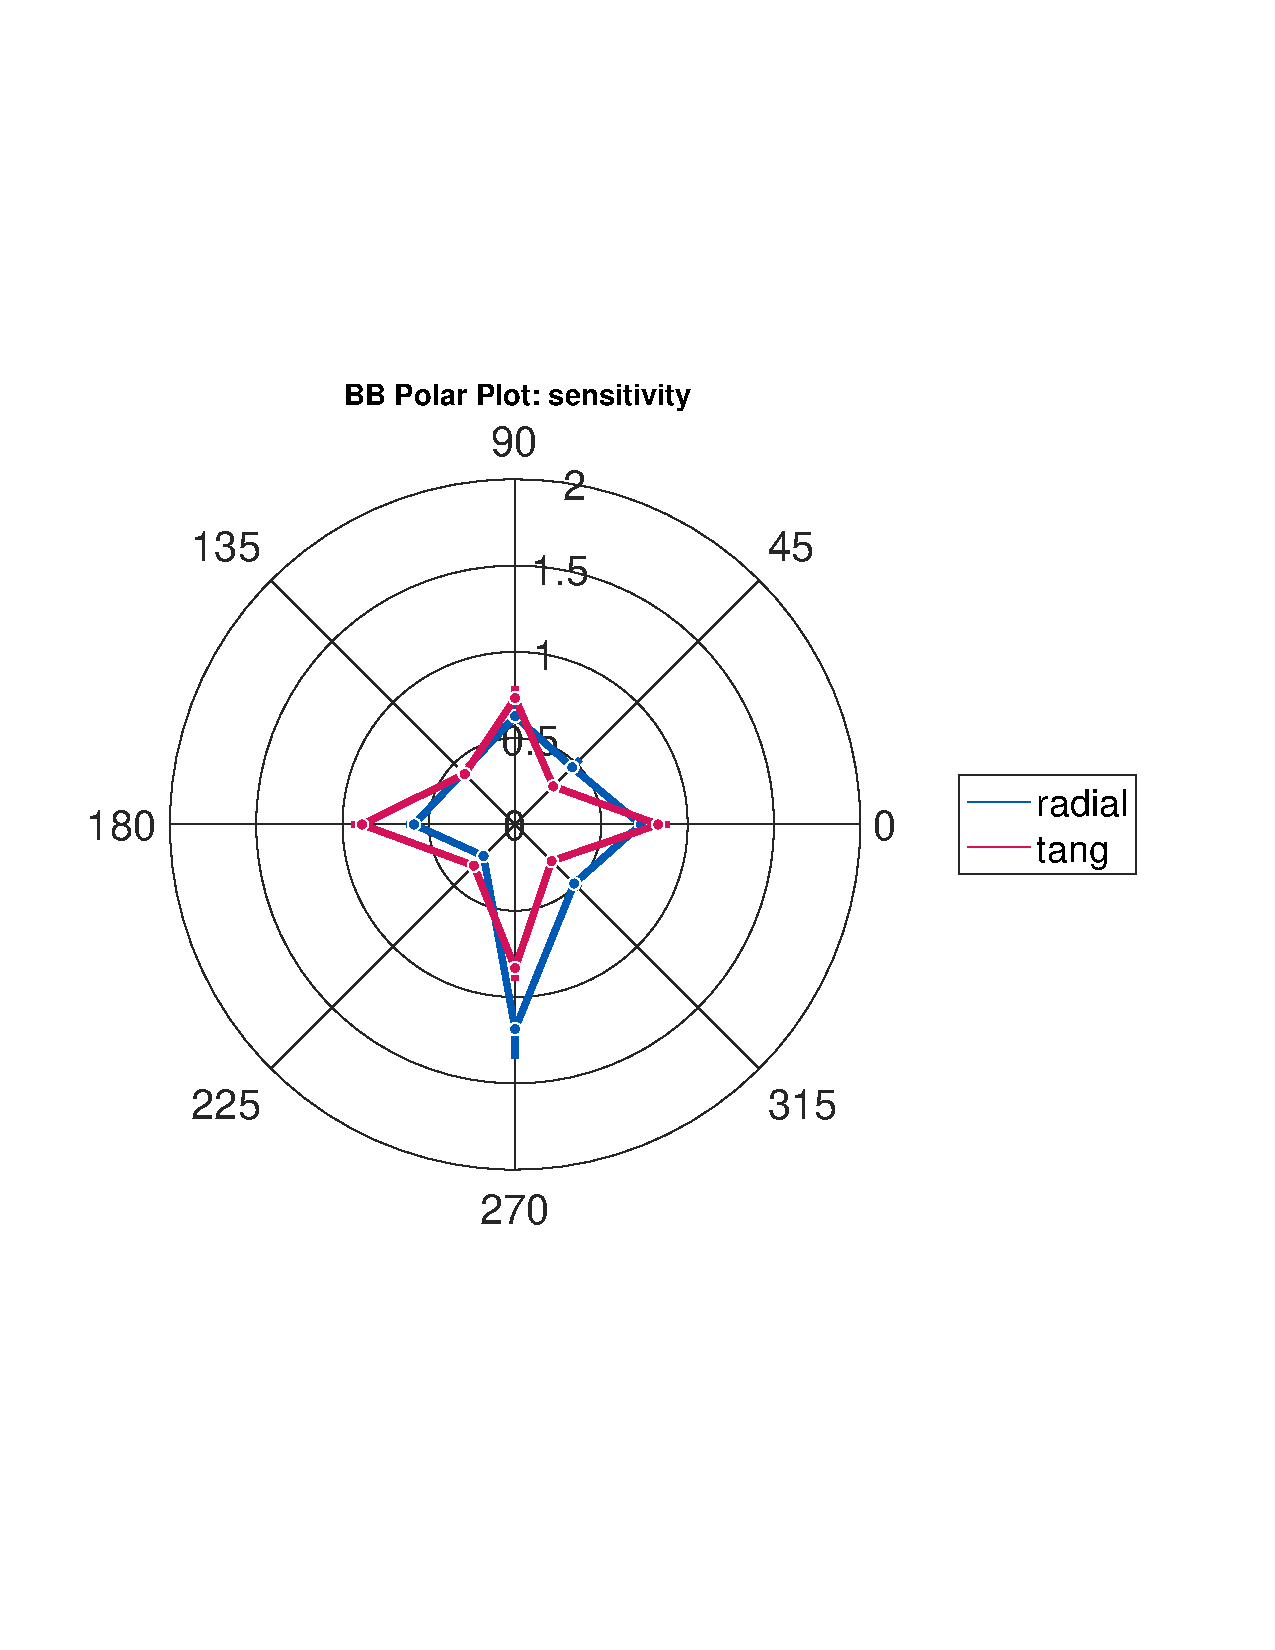
\includegraphics[scale=.3]{Images/BB_PP_sensitivity_Alldata_2conds_relative.png}
\end{figure}
\begin{figure}[H]
\centering % centers the figure
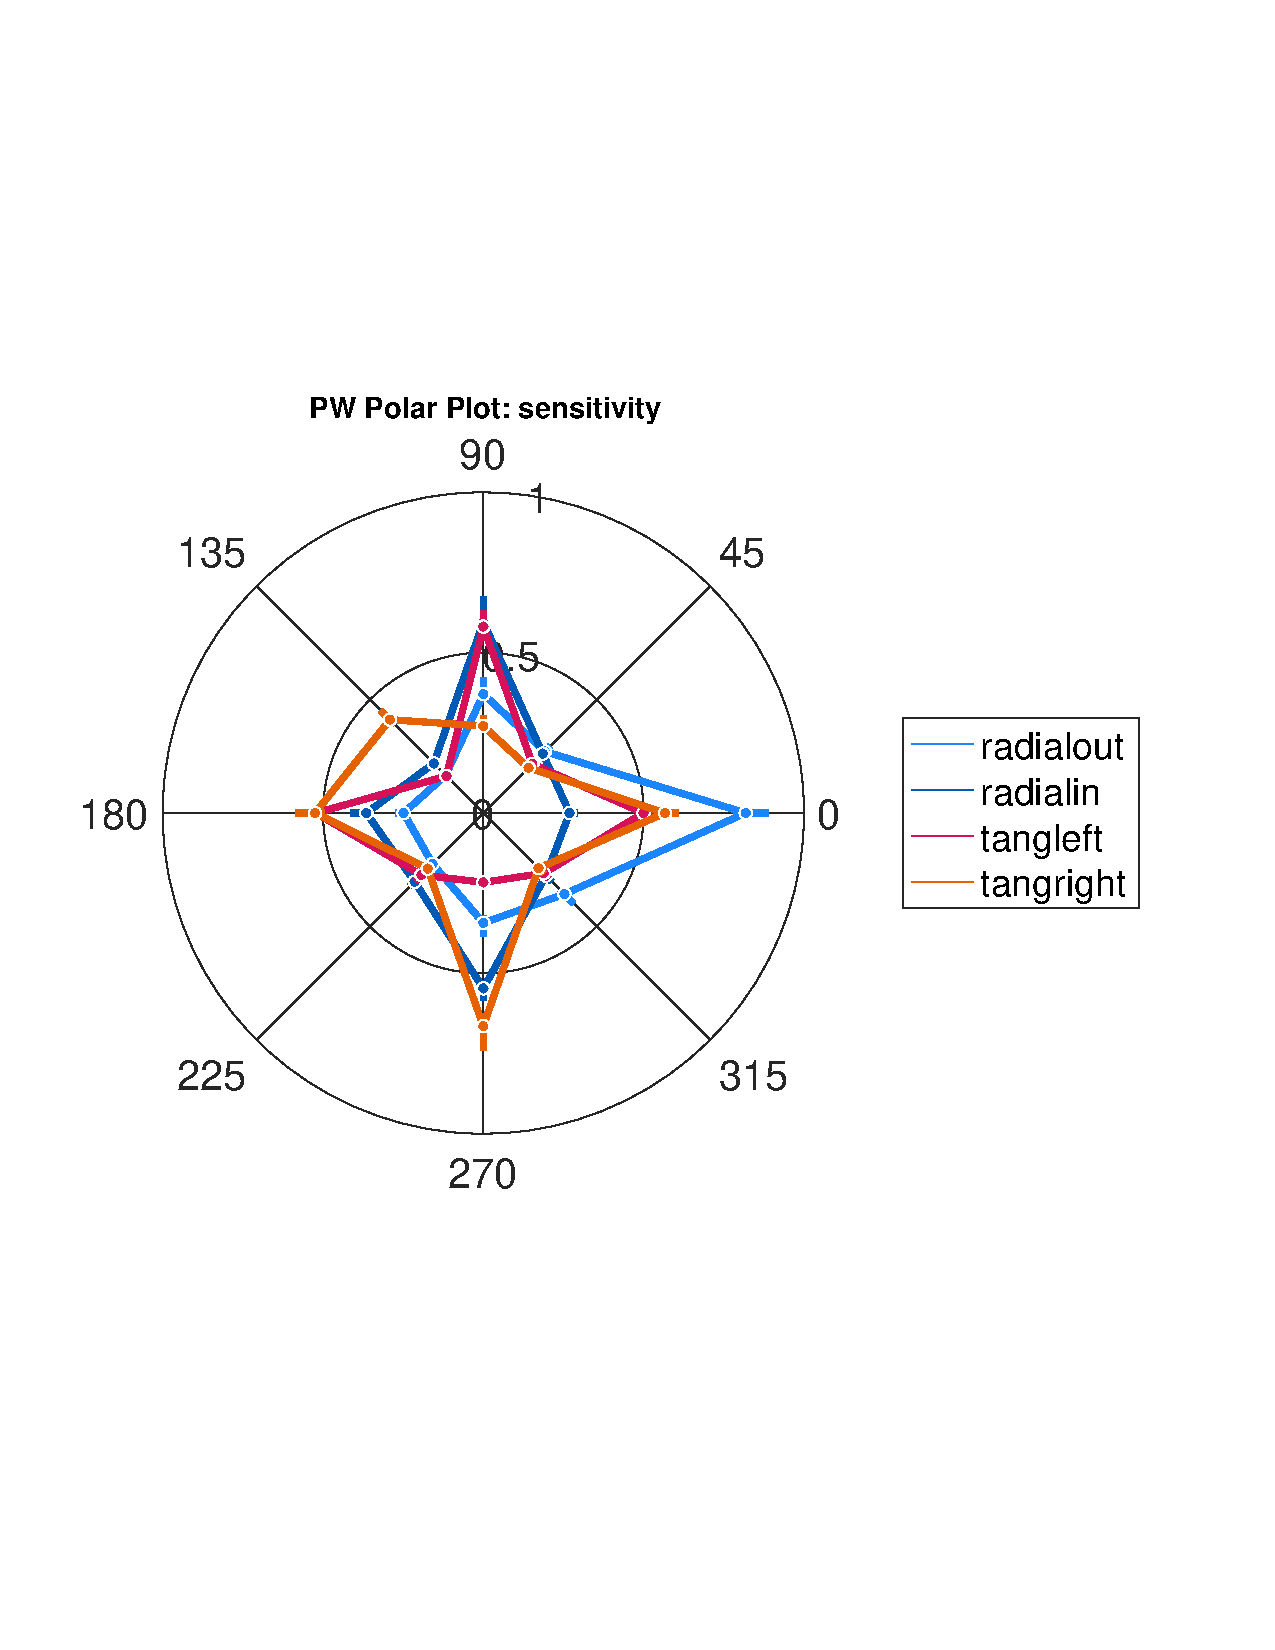
\includegraphics[scale=.3]{Images/PW_PP_sensitivity_Alldata_4conds_relative.png}
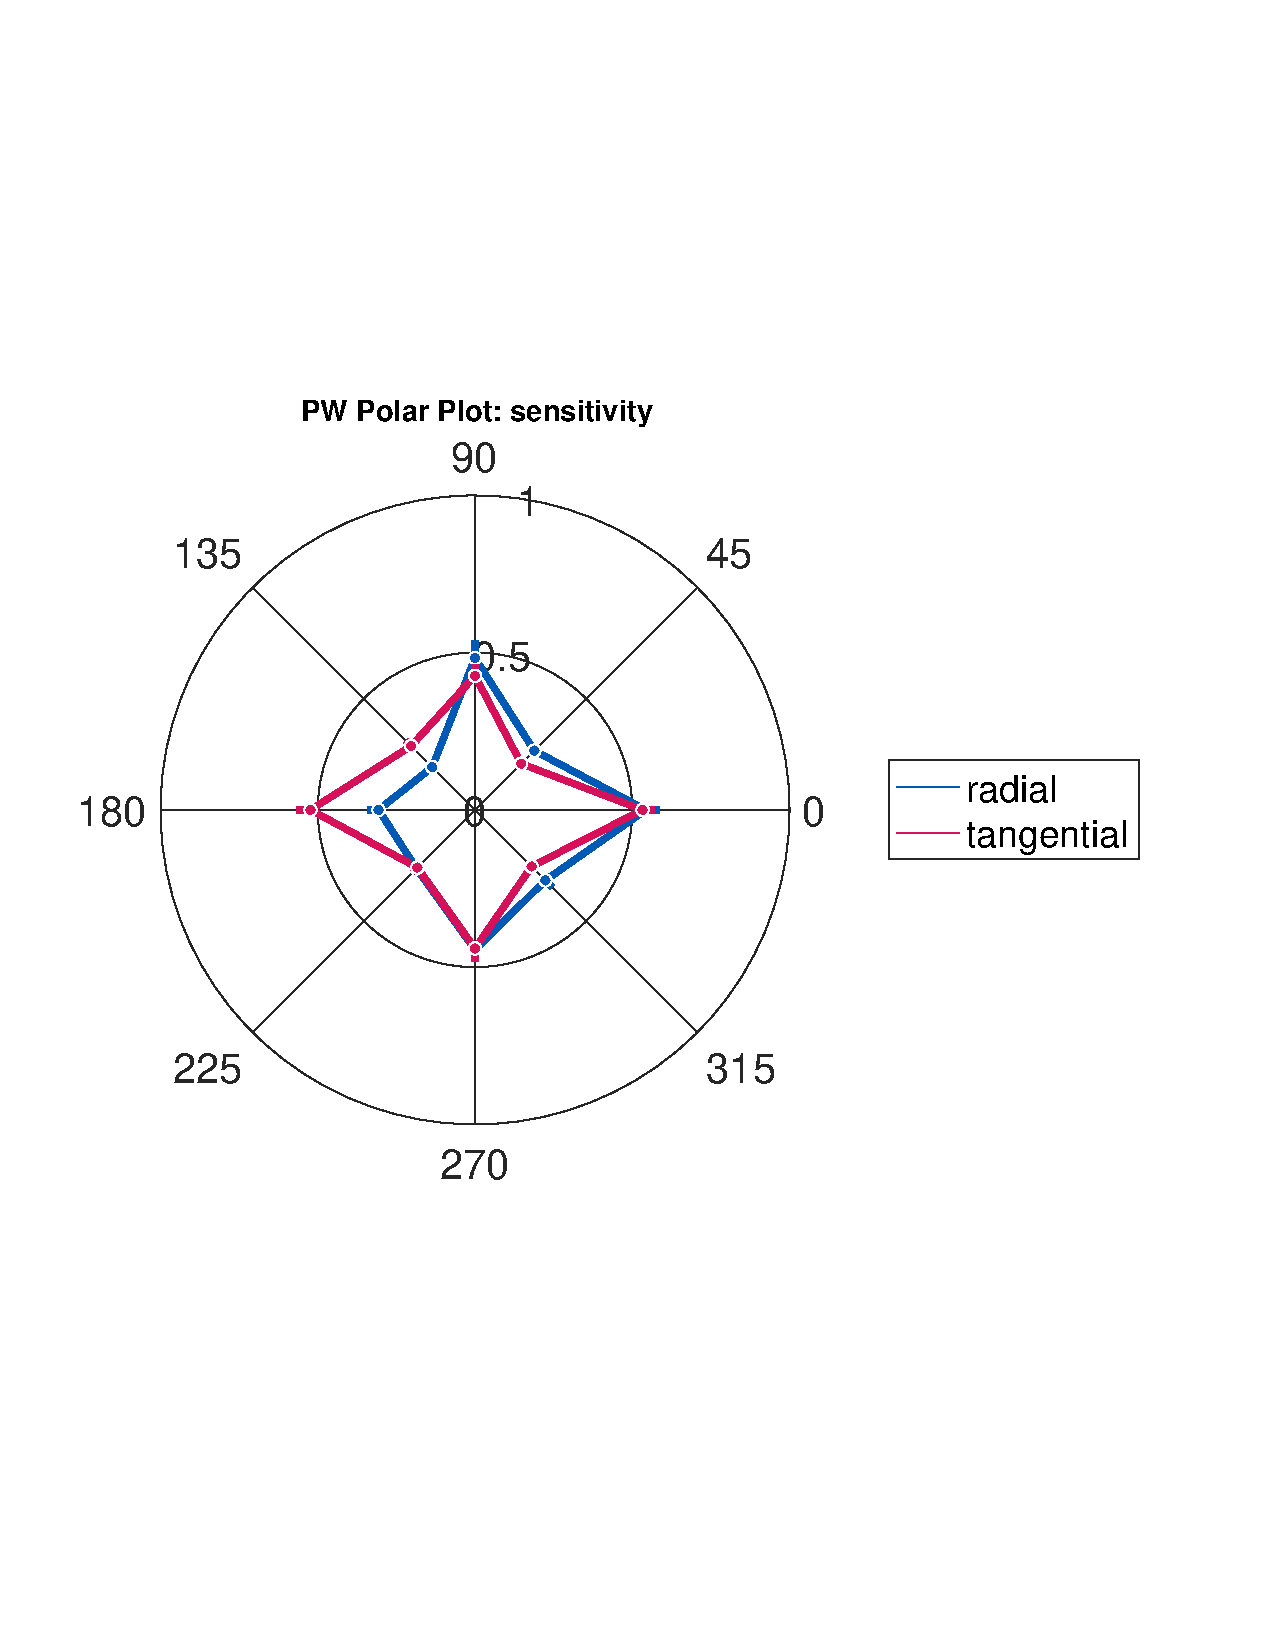
\includegraphics[scale=.3]{Images/PW_PP_sensitivity_Alldata_2conds_relative.png}
\end{figure}
\begin{figure}[H]
\centering % centers the figure
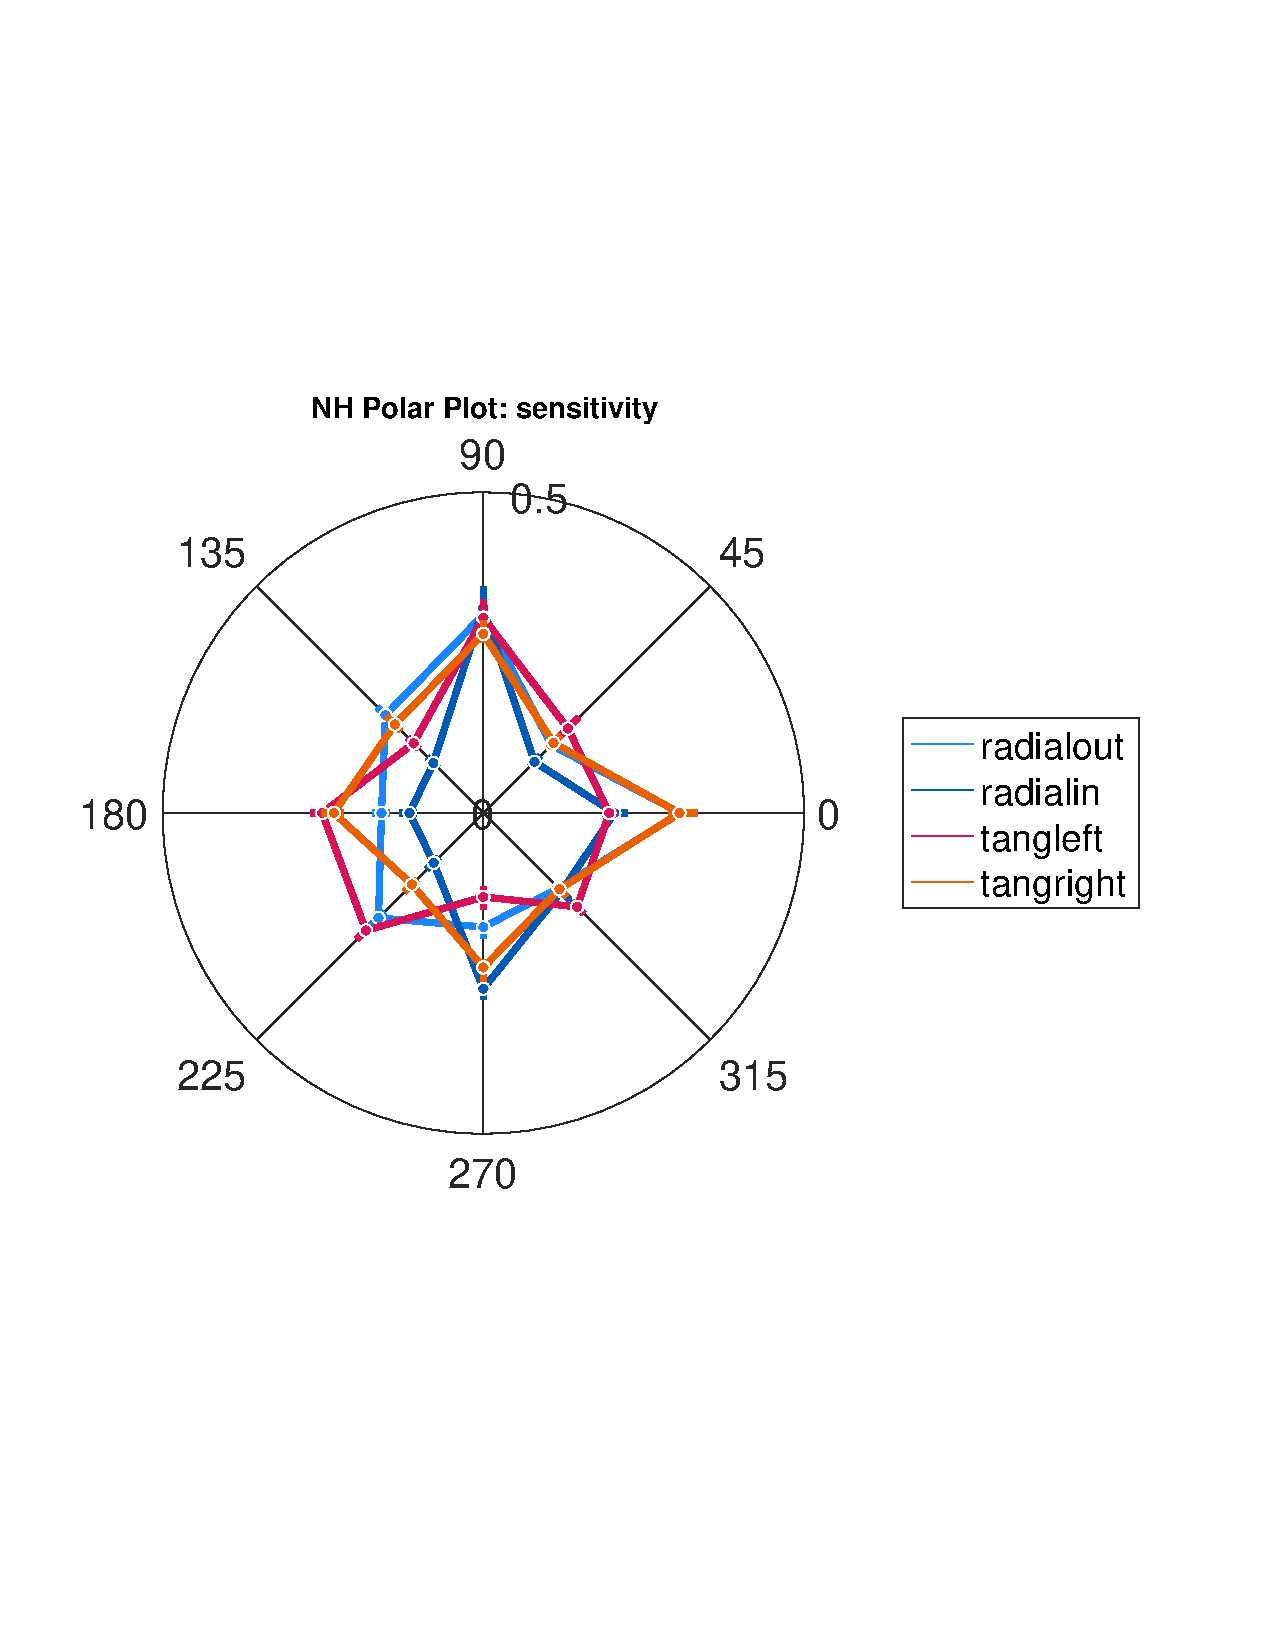
\includegraphics[scale=.3]{Images/NH_PP_sensitivity_Alldata_4conds_relative.png}
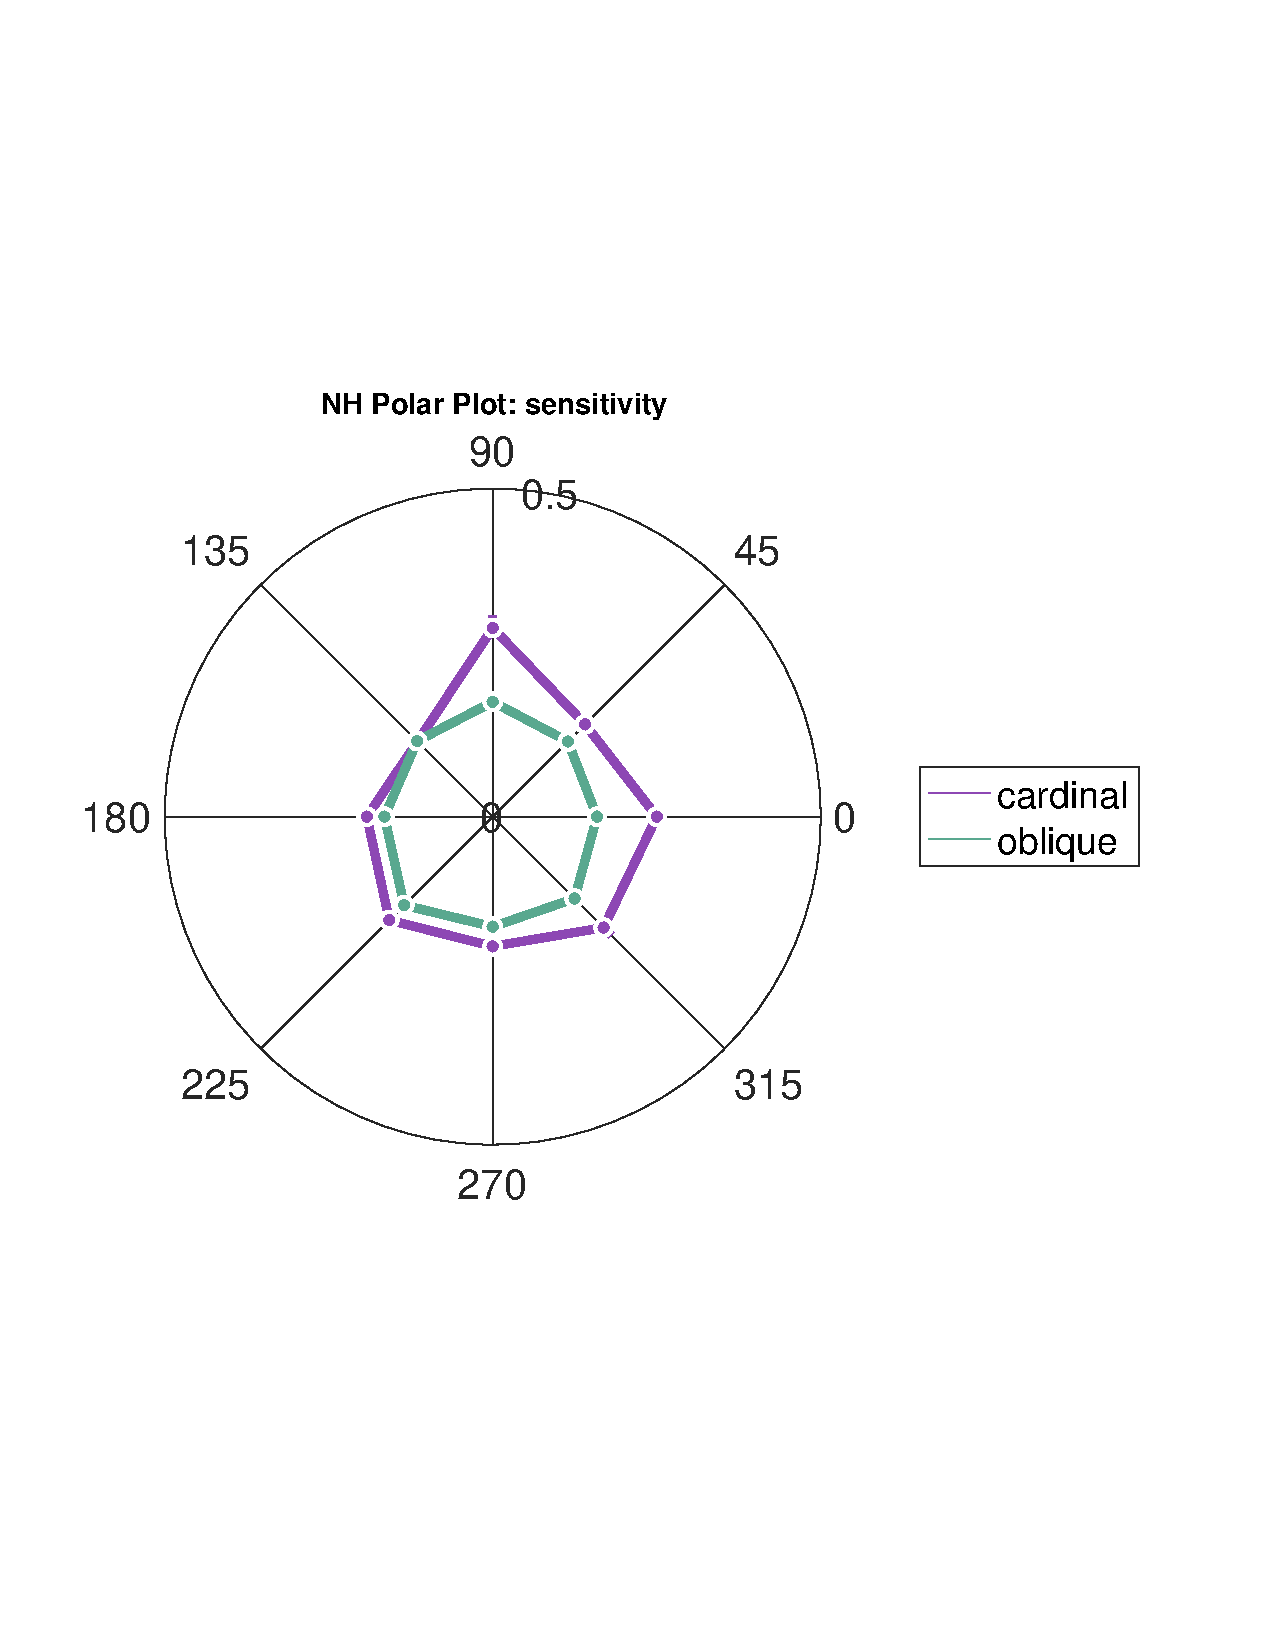
\includegraphics[scale=.3]{Images/NH_PP_sensitivity_Alldata_2conds_relative.png}
\caption{LEFT: 200 trials per point. RIGHT: 400 trials per point. 68\% CI from 1000 bootstraps.}
\end{figure}

\newpage
\subsection{Bias (absv) Polar Plots: Relative Motion}
\begin{figure}[H]
\centering % centers the figure
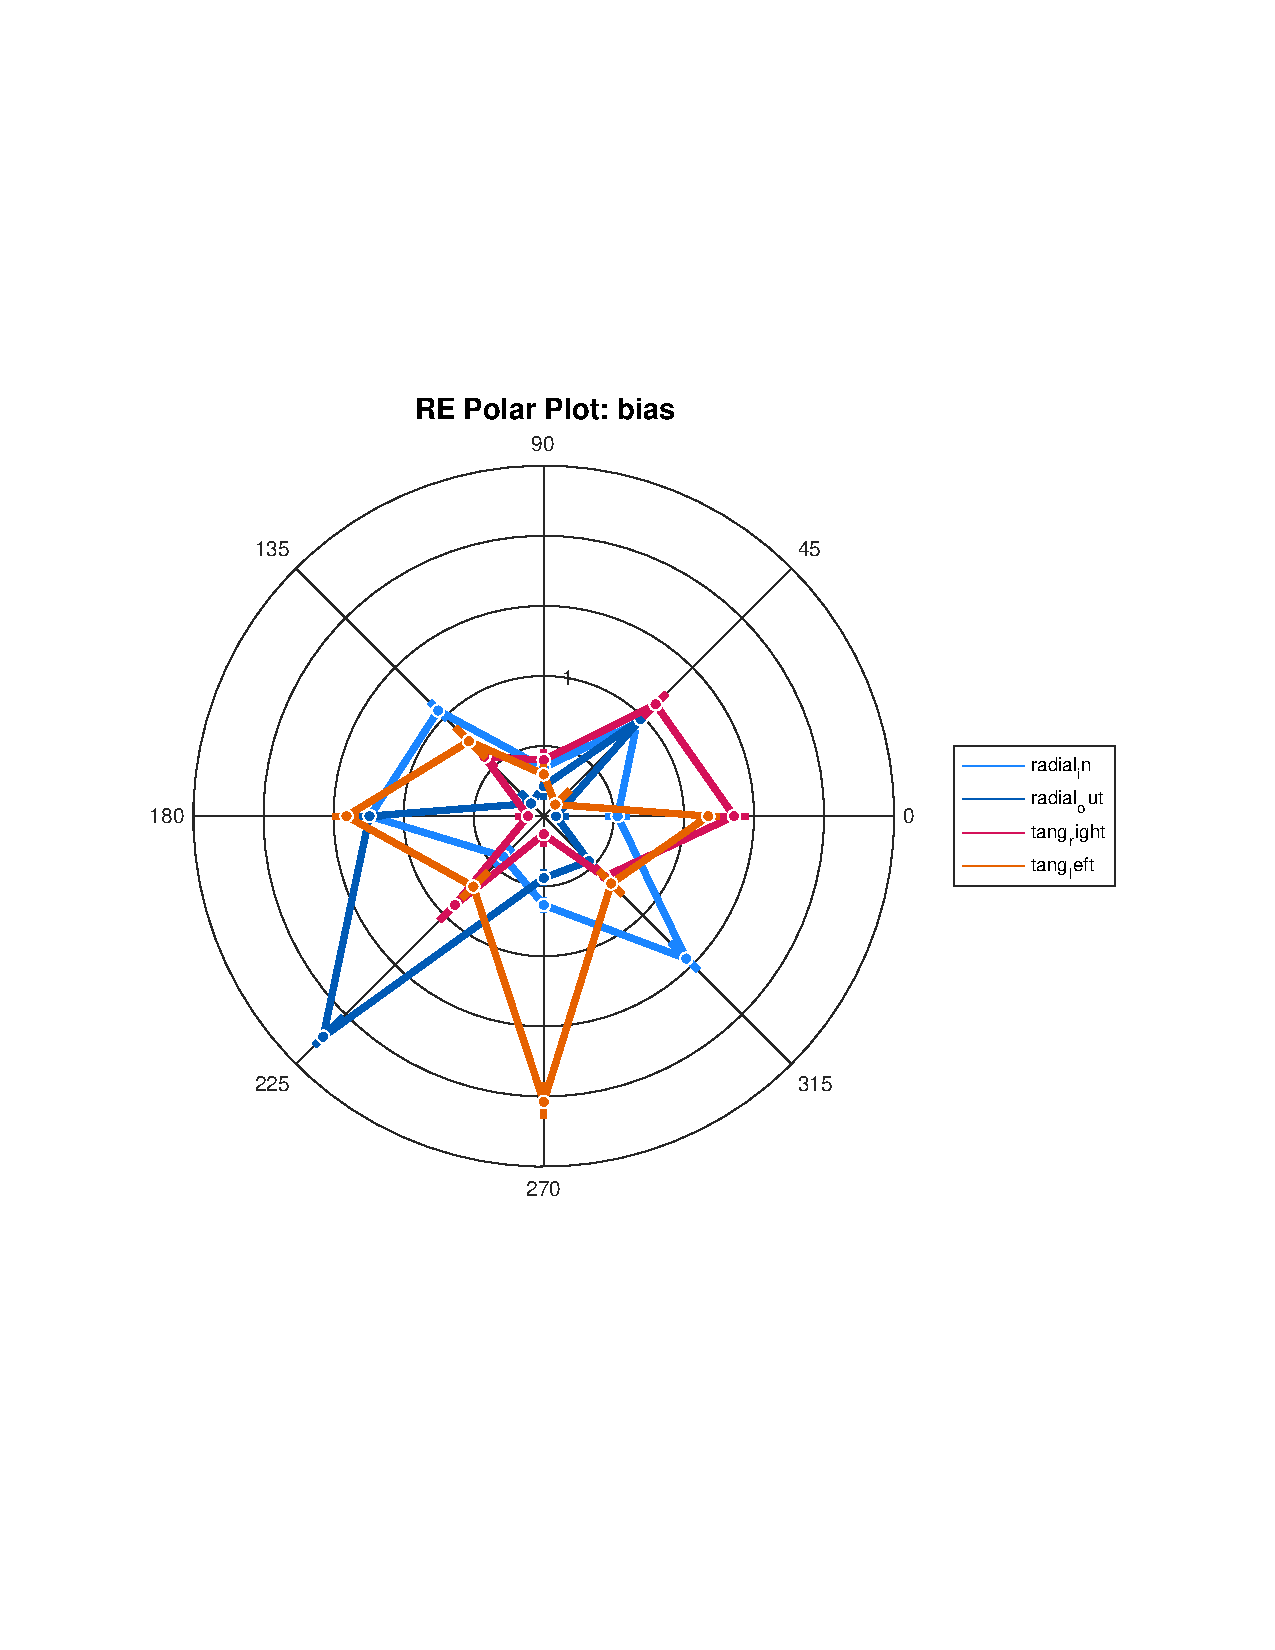
\includegraphics[scale=.3]{Images/RE_PP_bias_Alldata_4conds_relative.png}
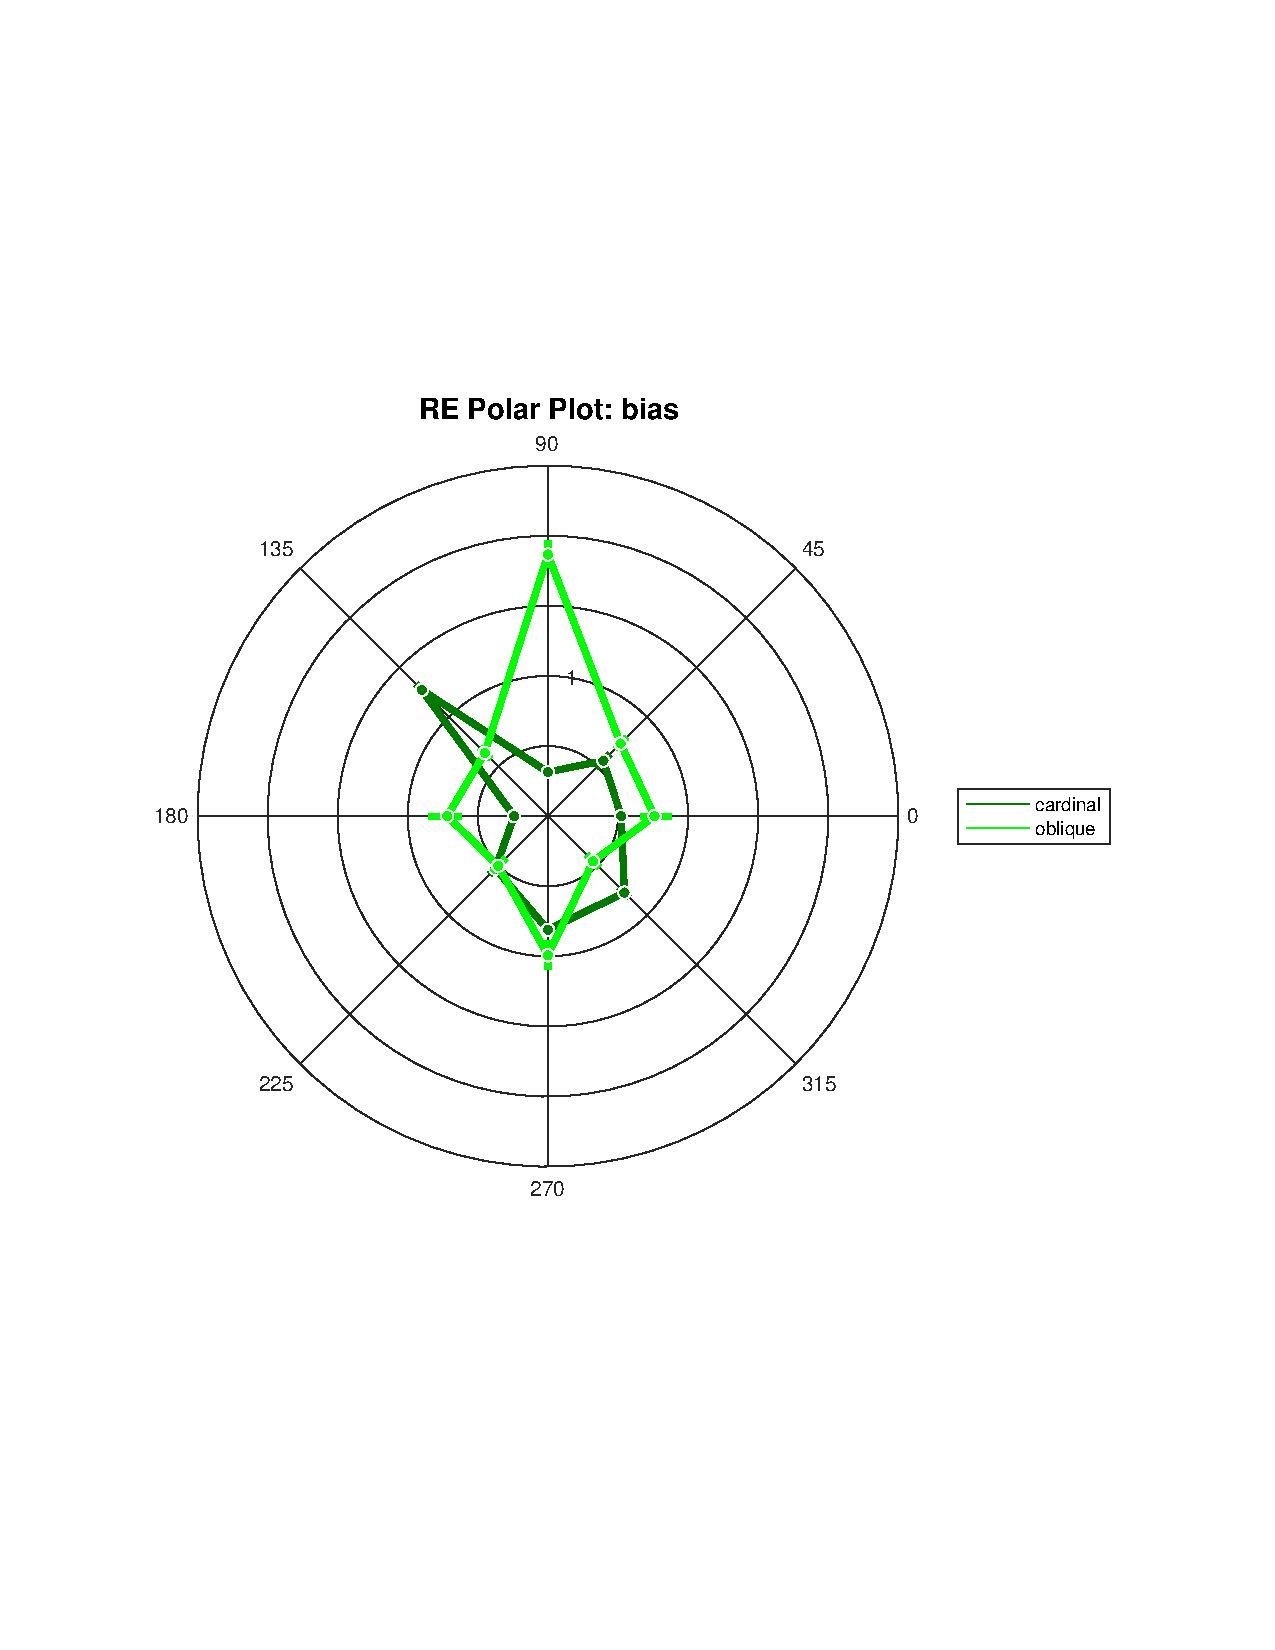
\includegraphics[scale=.3]{Images/RE_PP_bias_Alldata_2conds_relative.png}
\end{figure}
\begin{figure}[H]
\centering % centers the figure
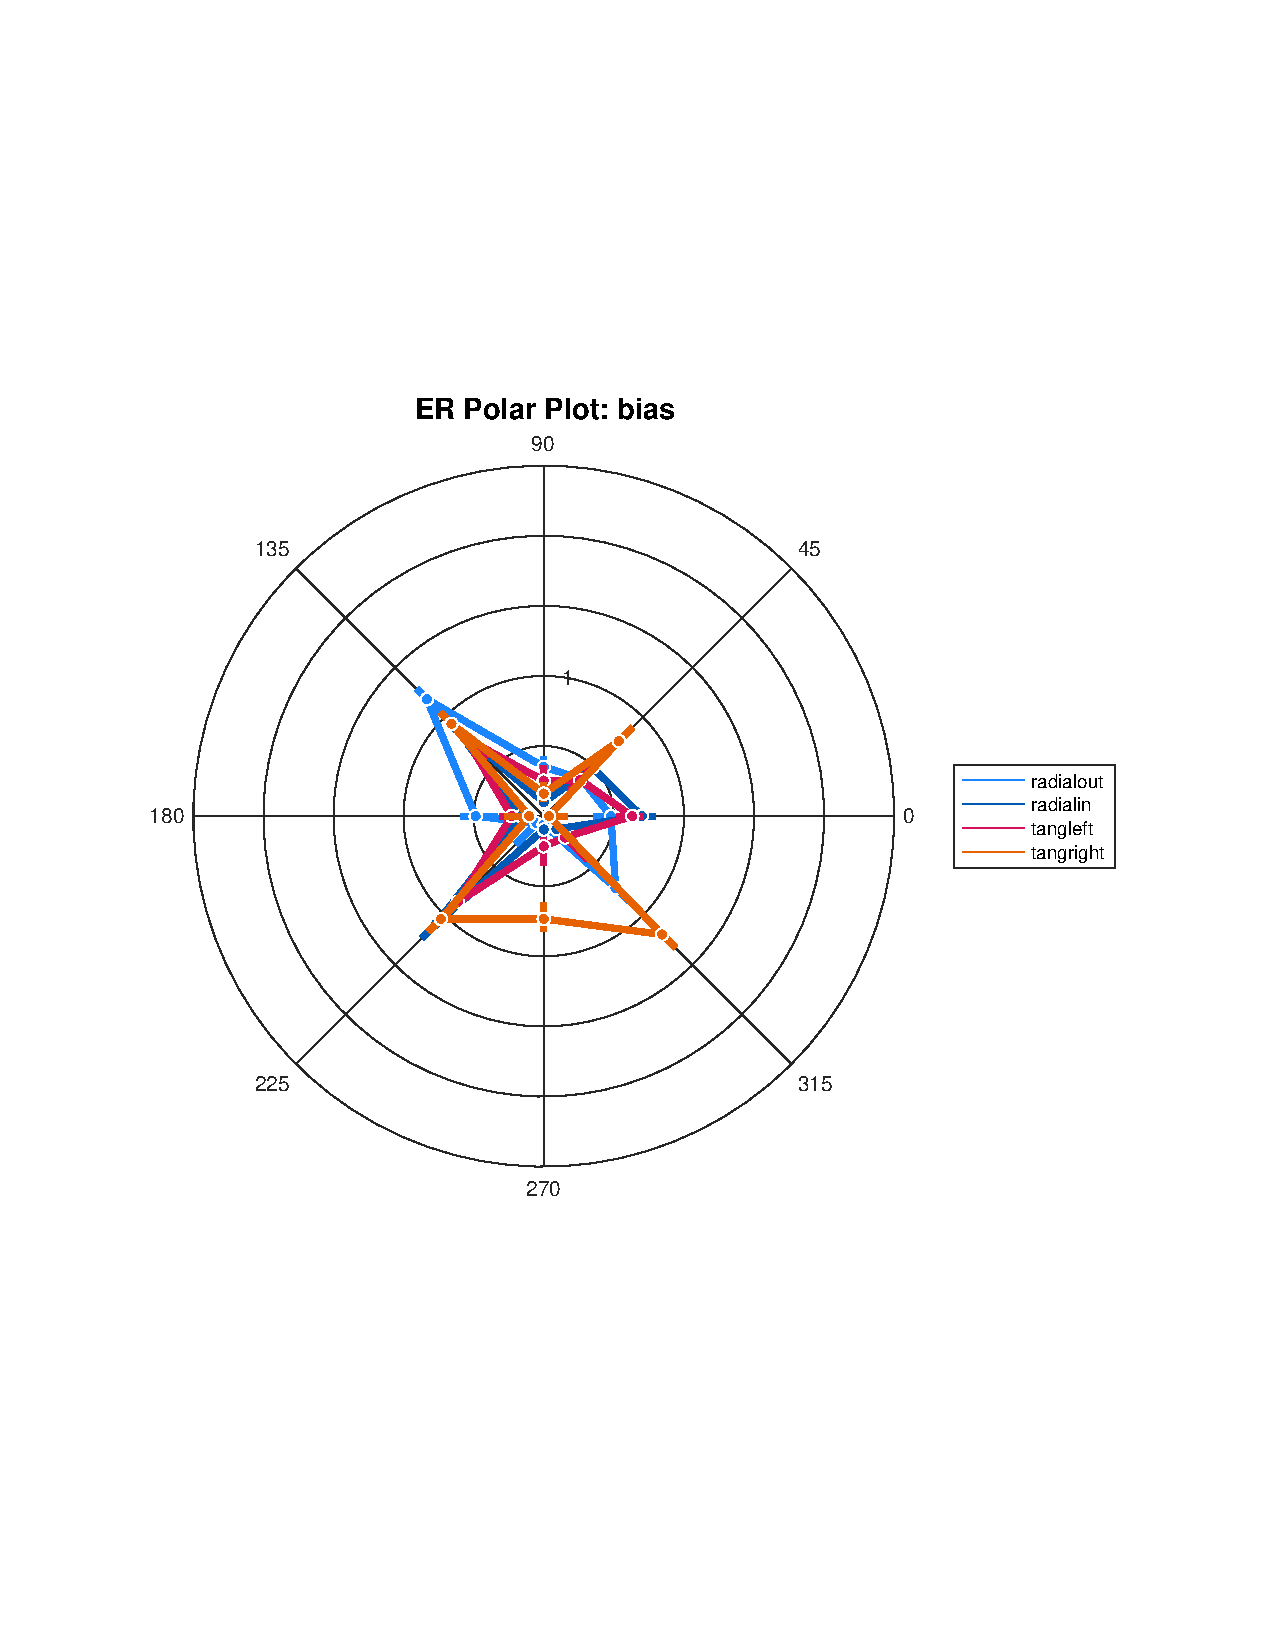
\includegraphics[scale=.3]{Images/ER_PP_bias_Alldata_4conds_relative.png}
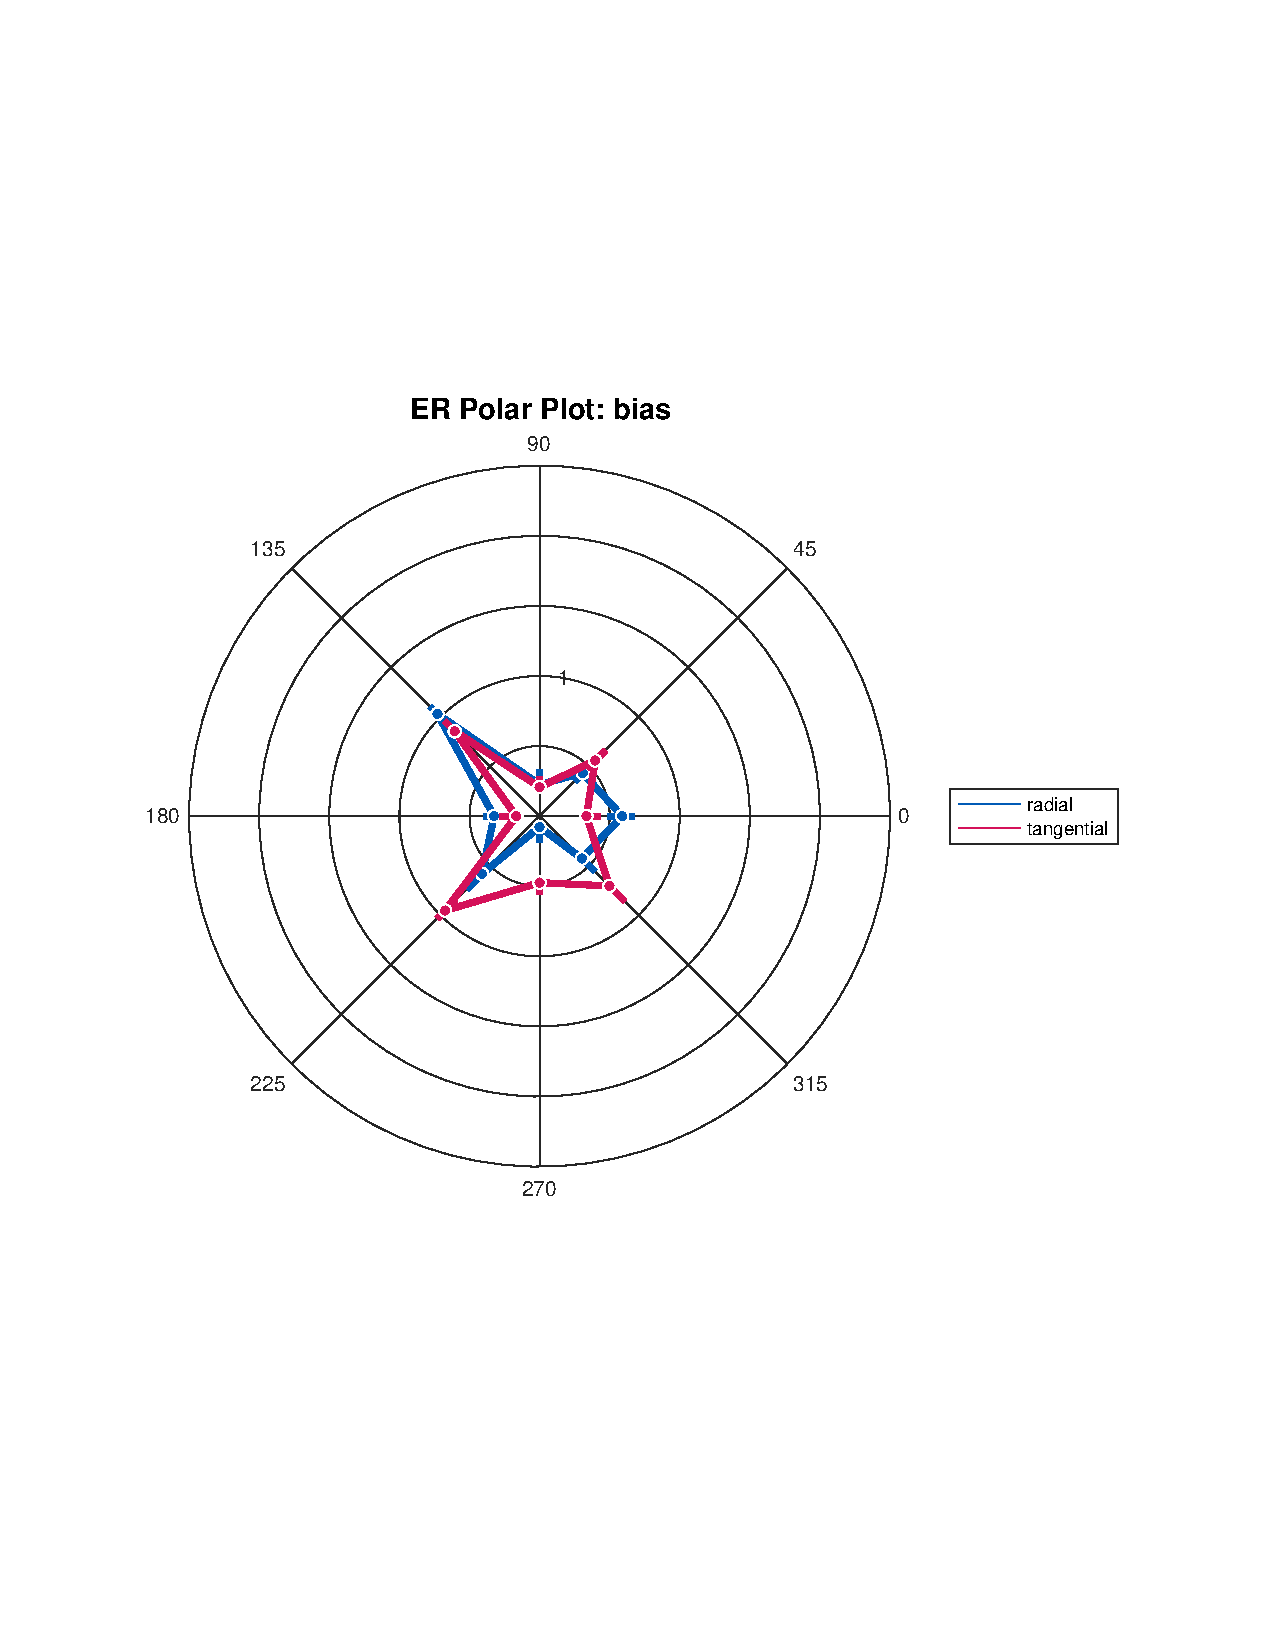
\includegraphics[scale=.3]{Images/ER_PP_bias_Alldata_2conds_relative.png}
\caption{Same subject (RE) but at half distance.}
\end{figure}
\begin{figure}[H]
\centering % centers the figure
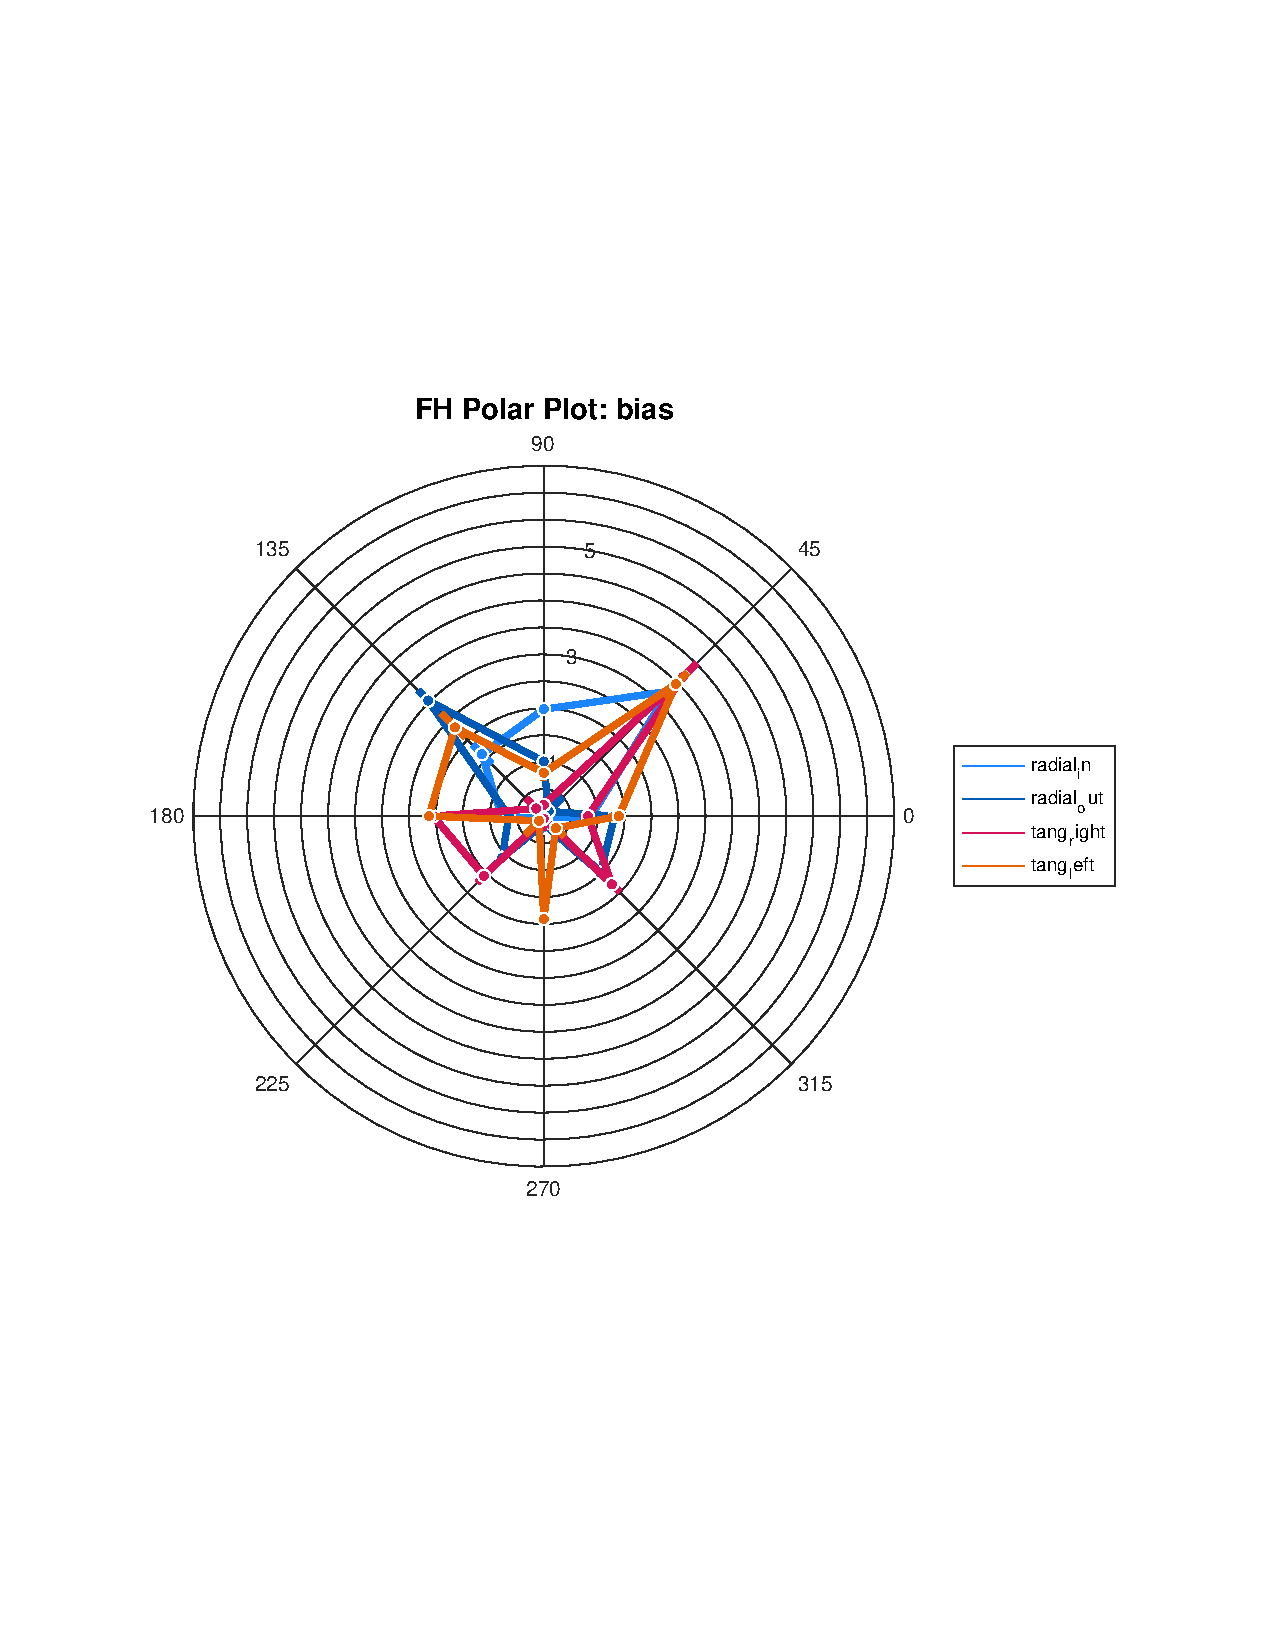
\includegraphics[scale=.3]{Images/FH_PP_bias_Alldata_4conds_relative.png}
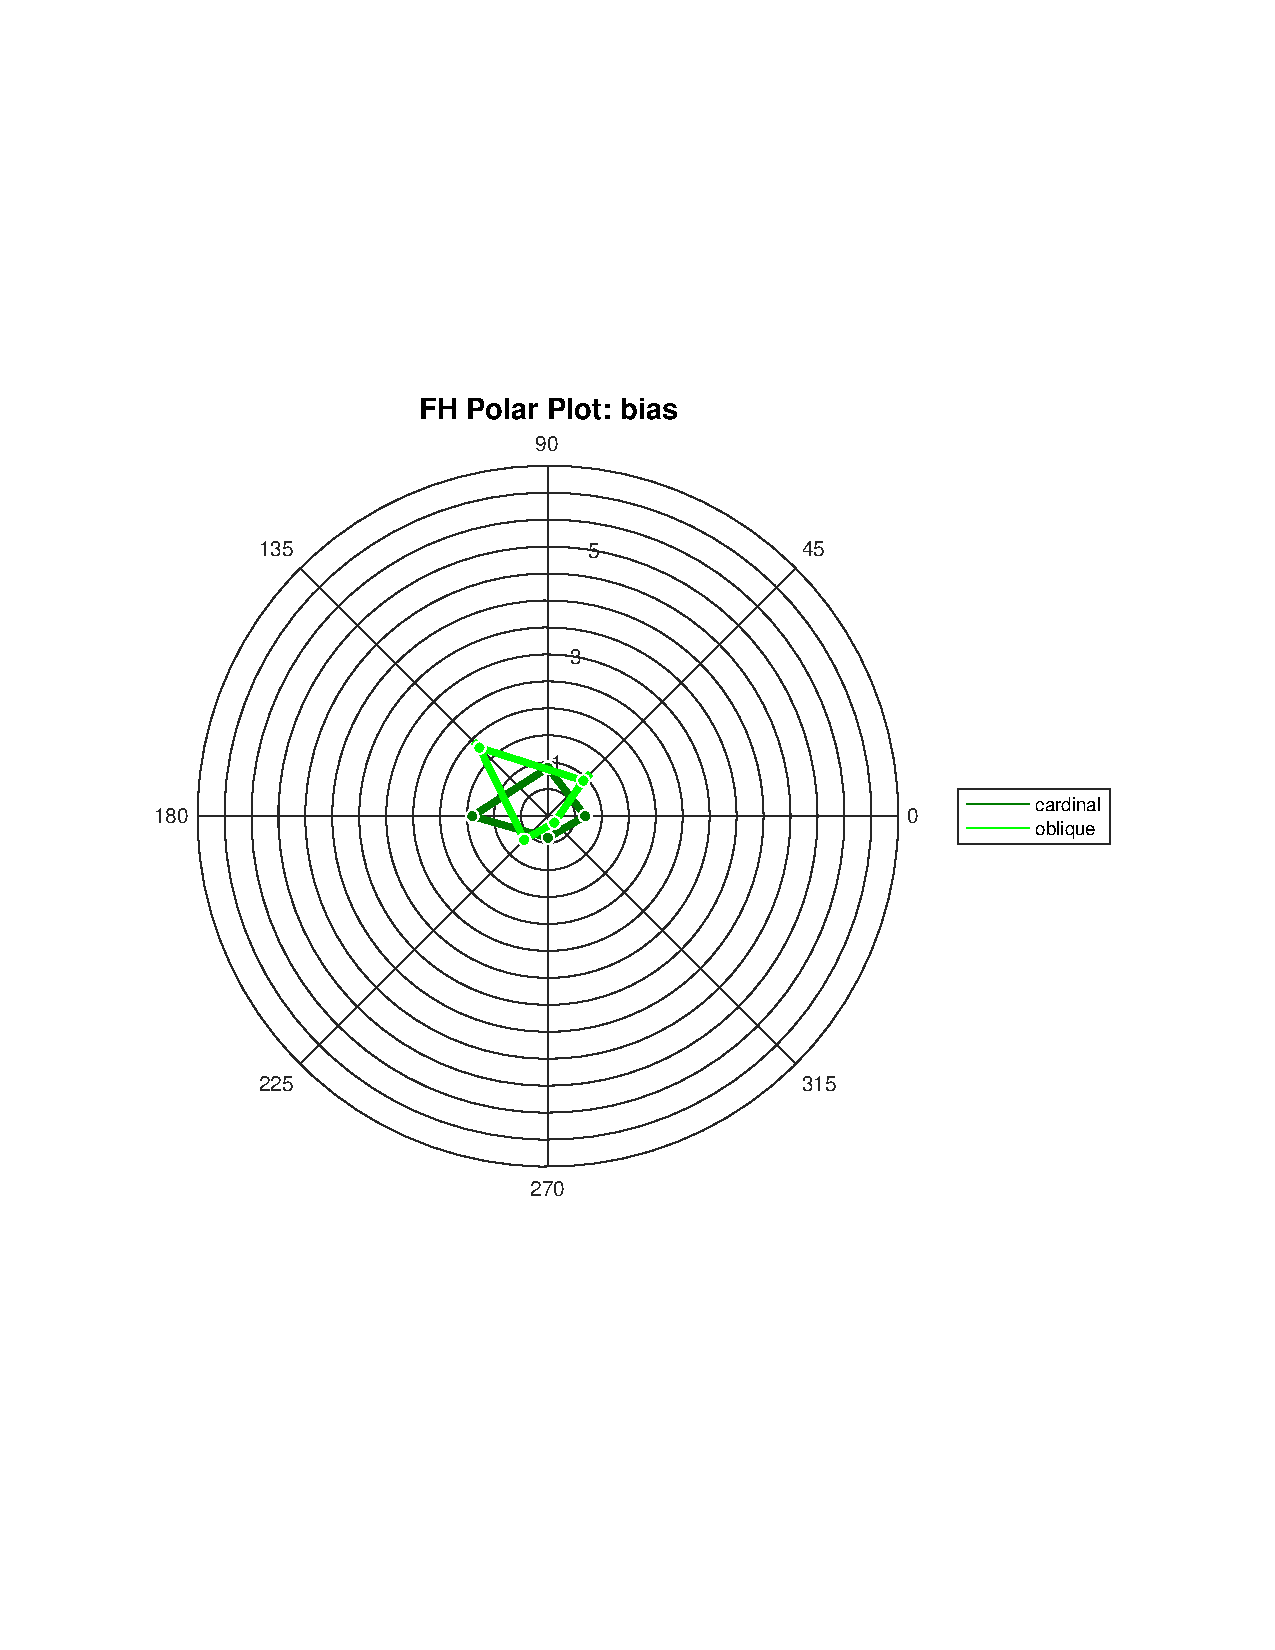
\includegraphics[scale=.3]{Images/FH_PP_bias_Alldata_2conds_relative.png}
\end{figure}
\begin{figure}[H]
\centering % centers the figure
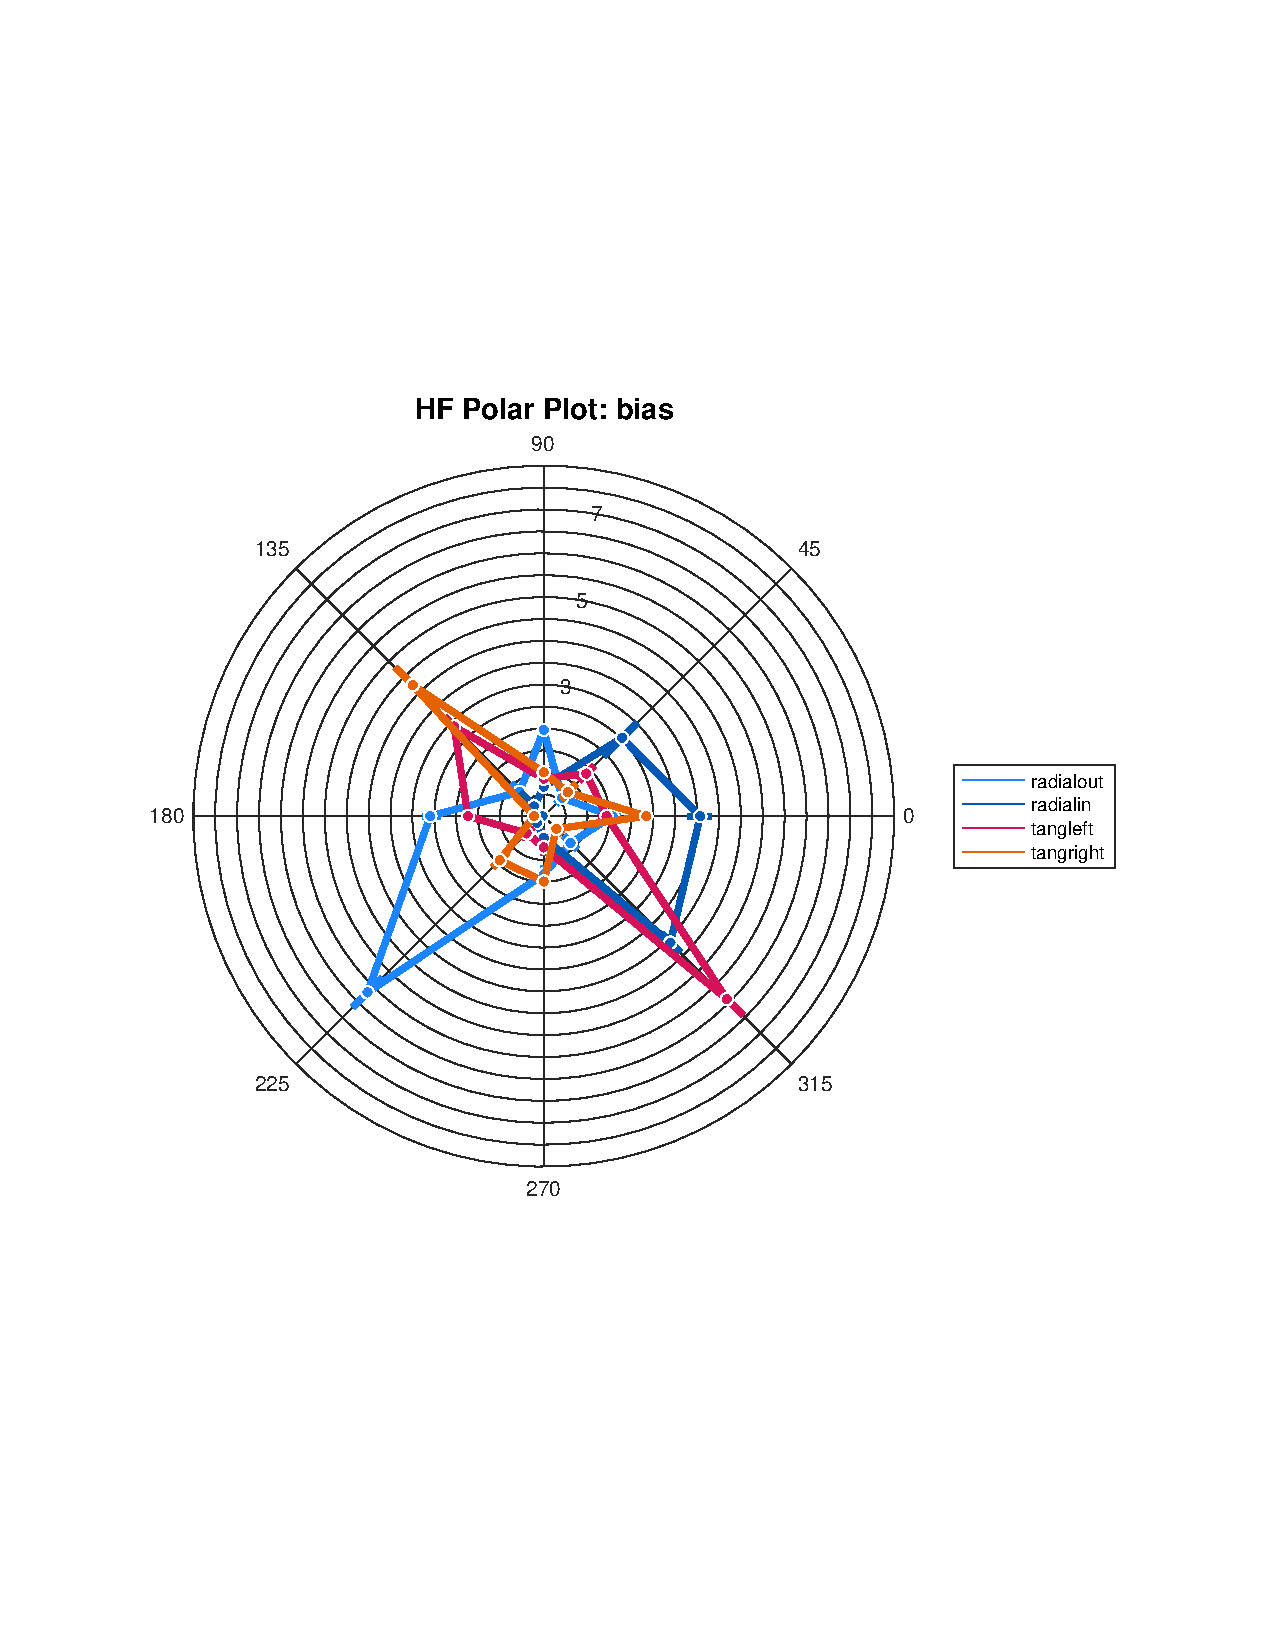
\includegraphics[scale=.3]{Images/HF_PP_bias_Alldata_4conds_relative.png}
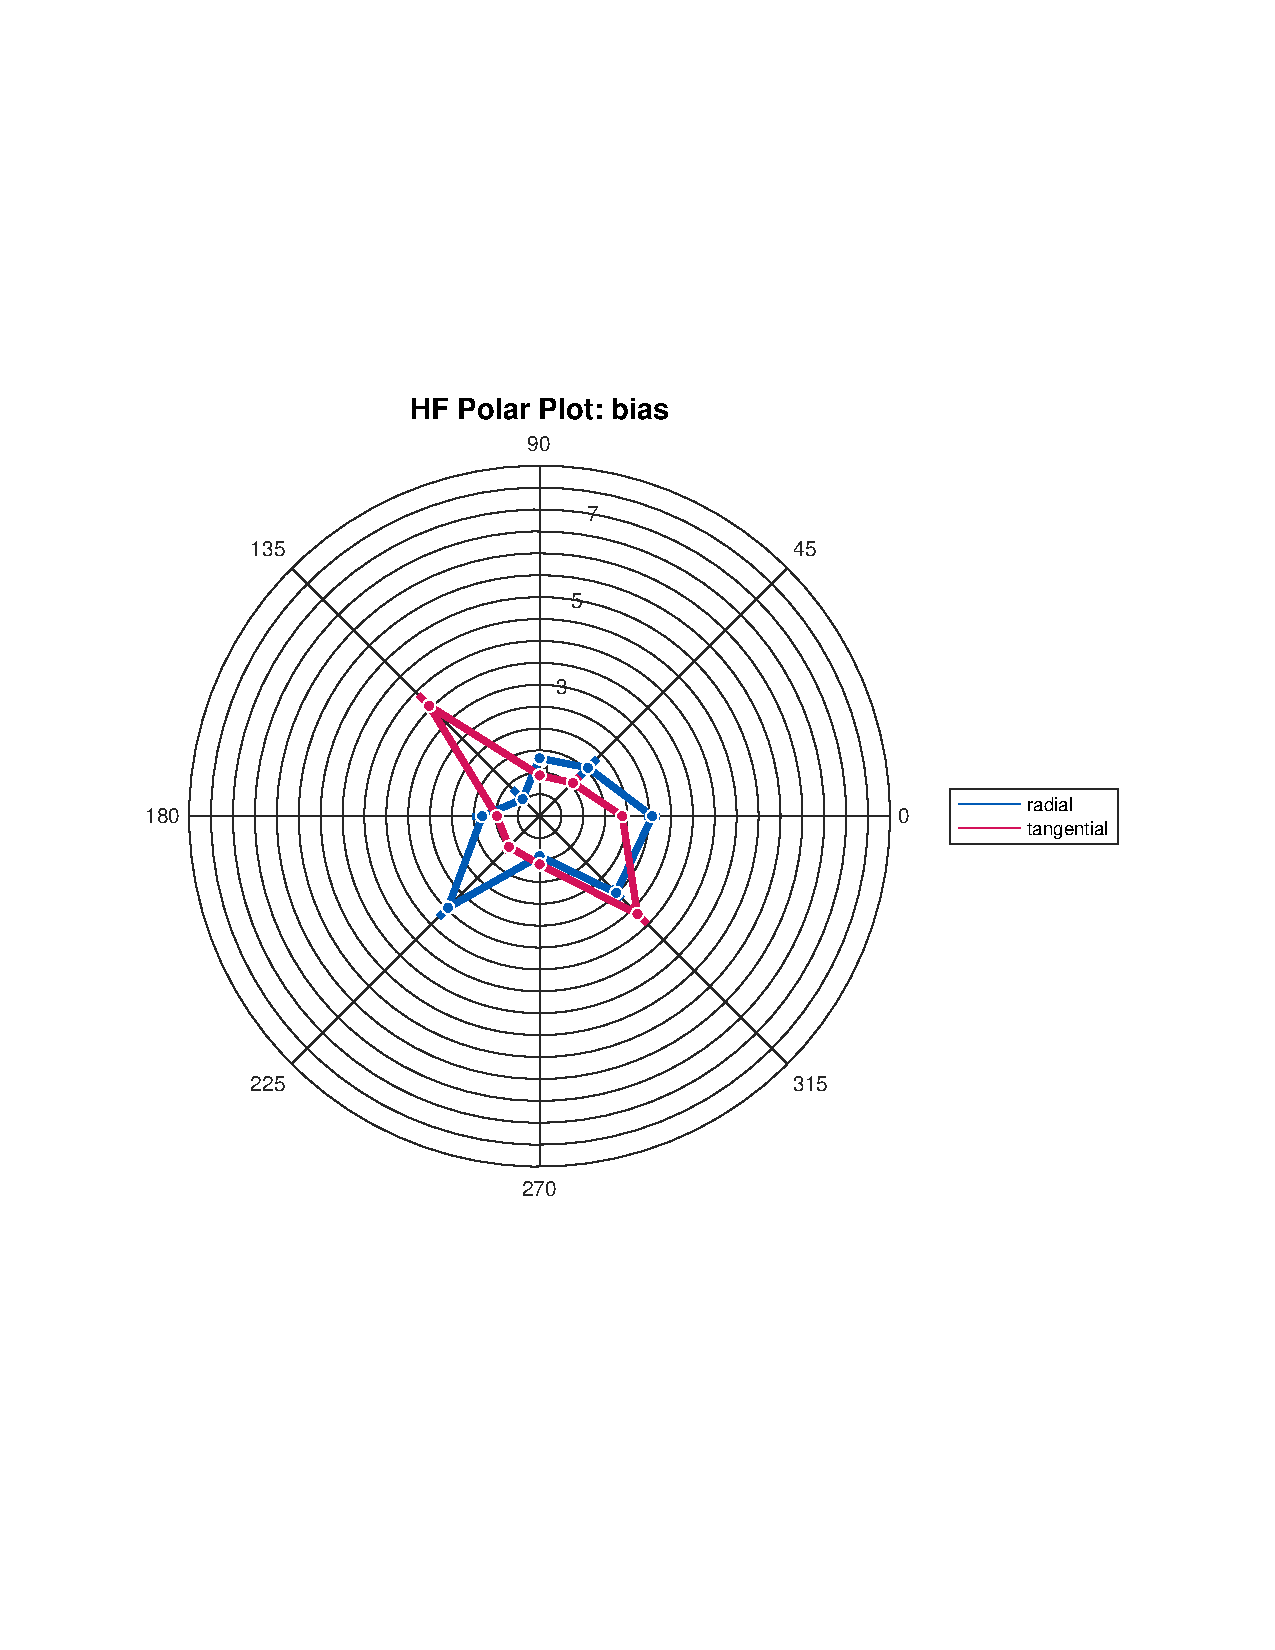
\includegraphics[scale=.3]{Images/HF_PP_bias_Alldata_2conds_relative.png}
\caption{Same subject (FH) but at half distance.}
\end{figure}
\begin{figure}[H]
\centering % centers the figure
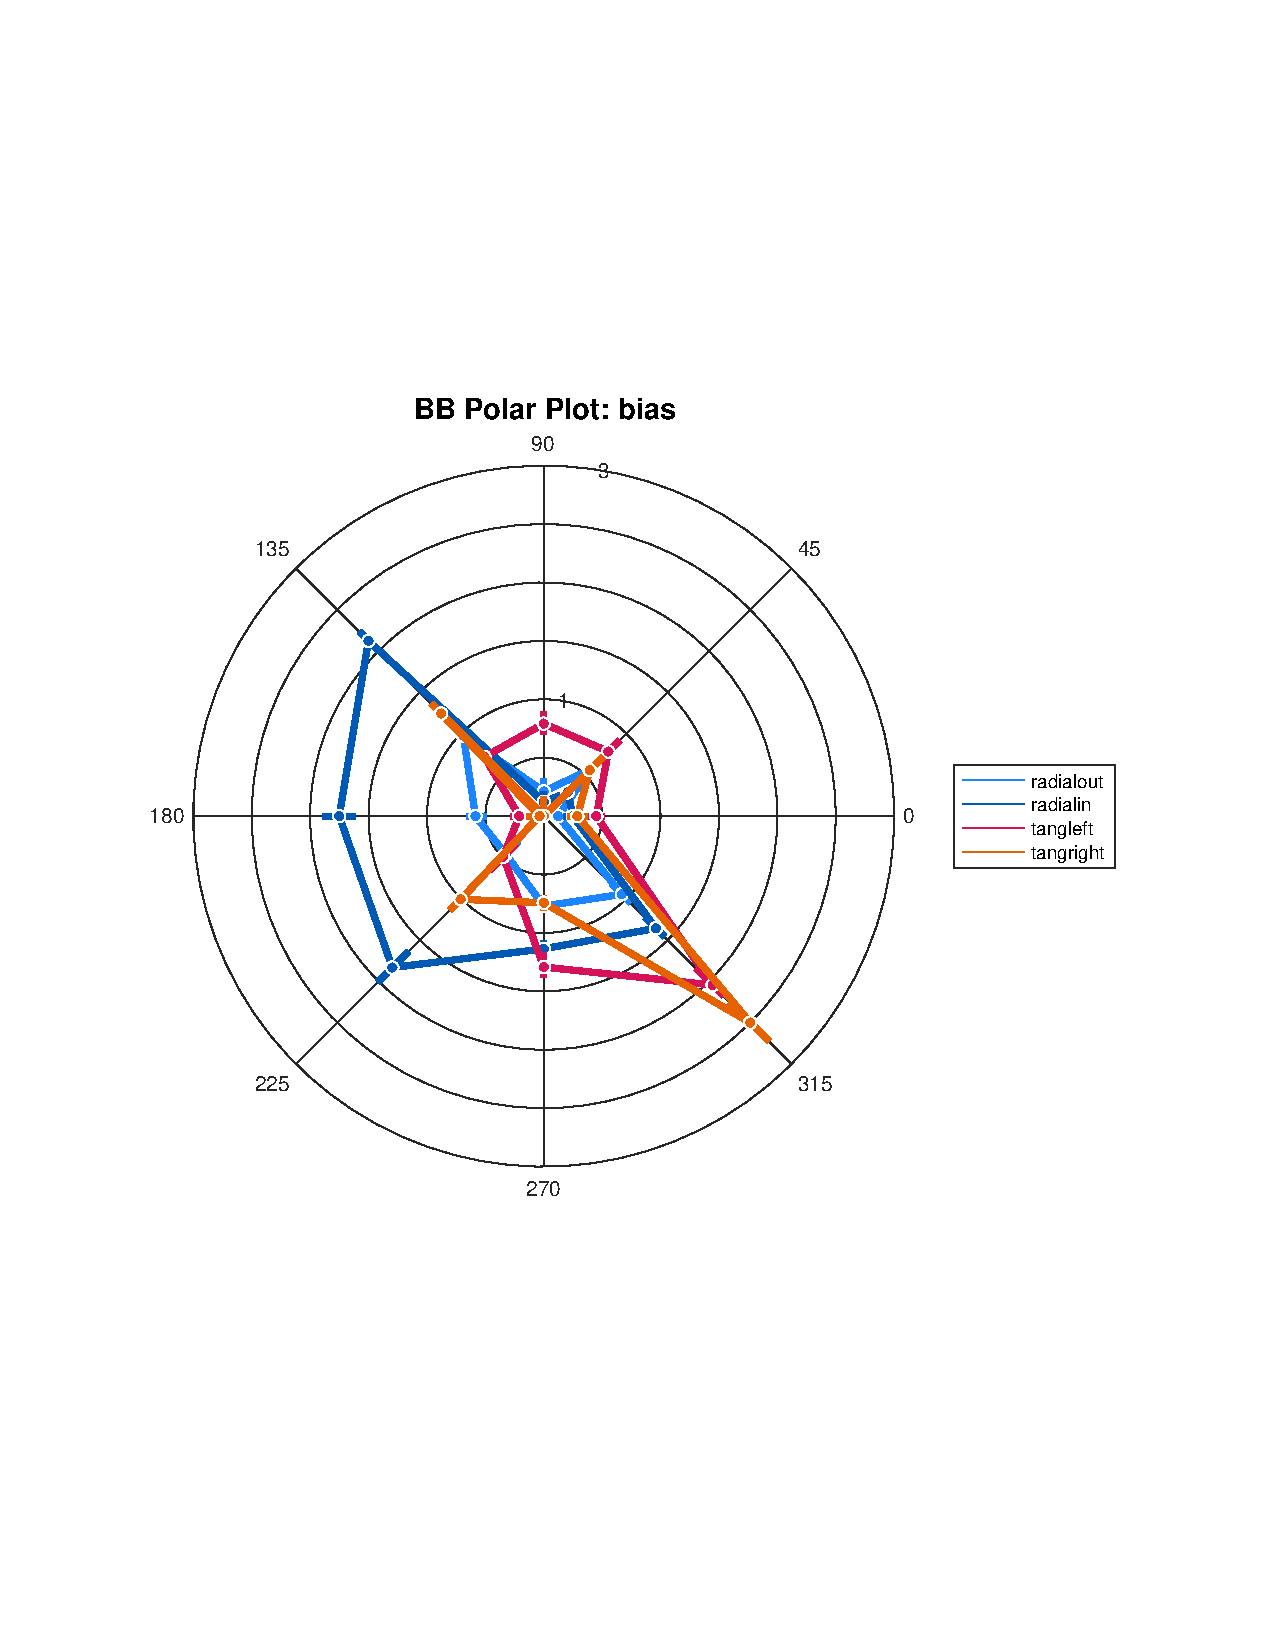
\includegraphics[scale=.3]{Images/BB_PP_bias_Alldata_4conds_relative.png}
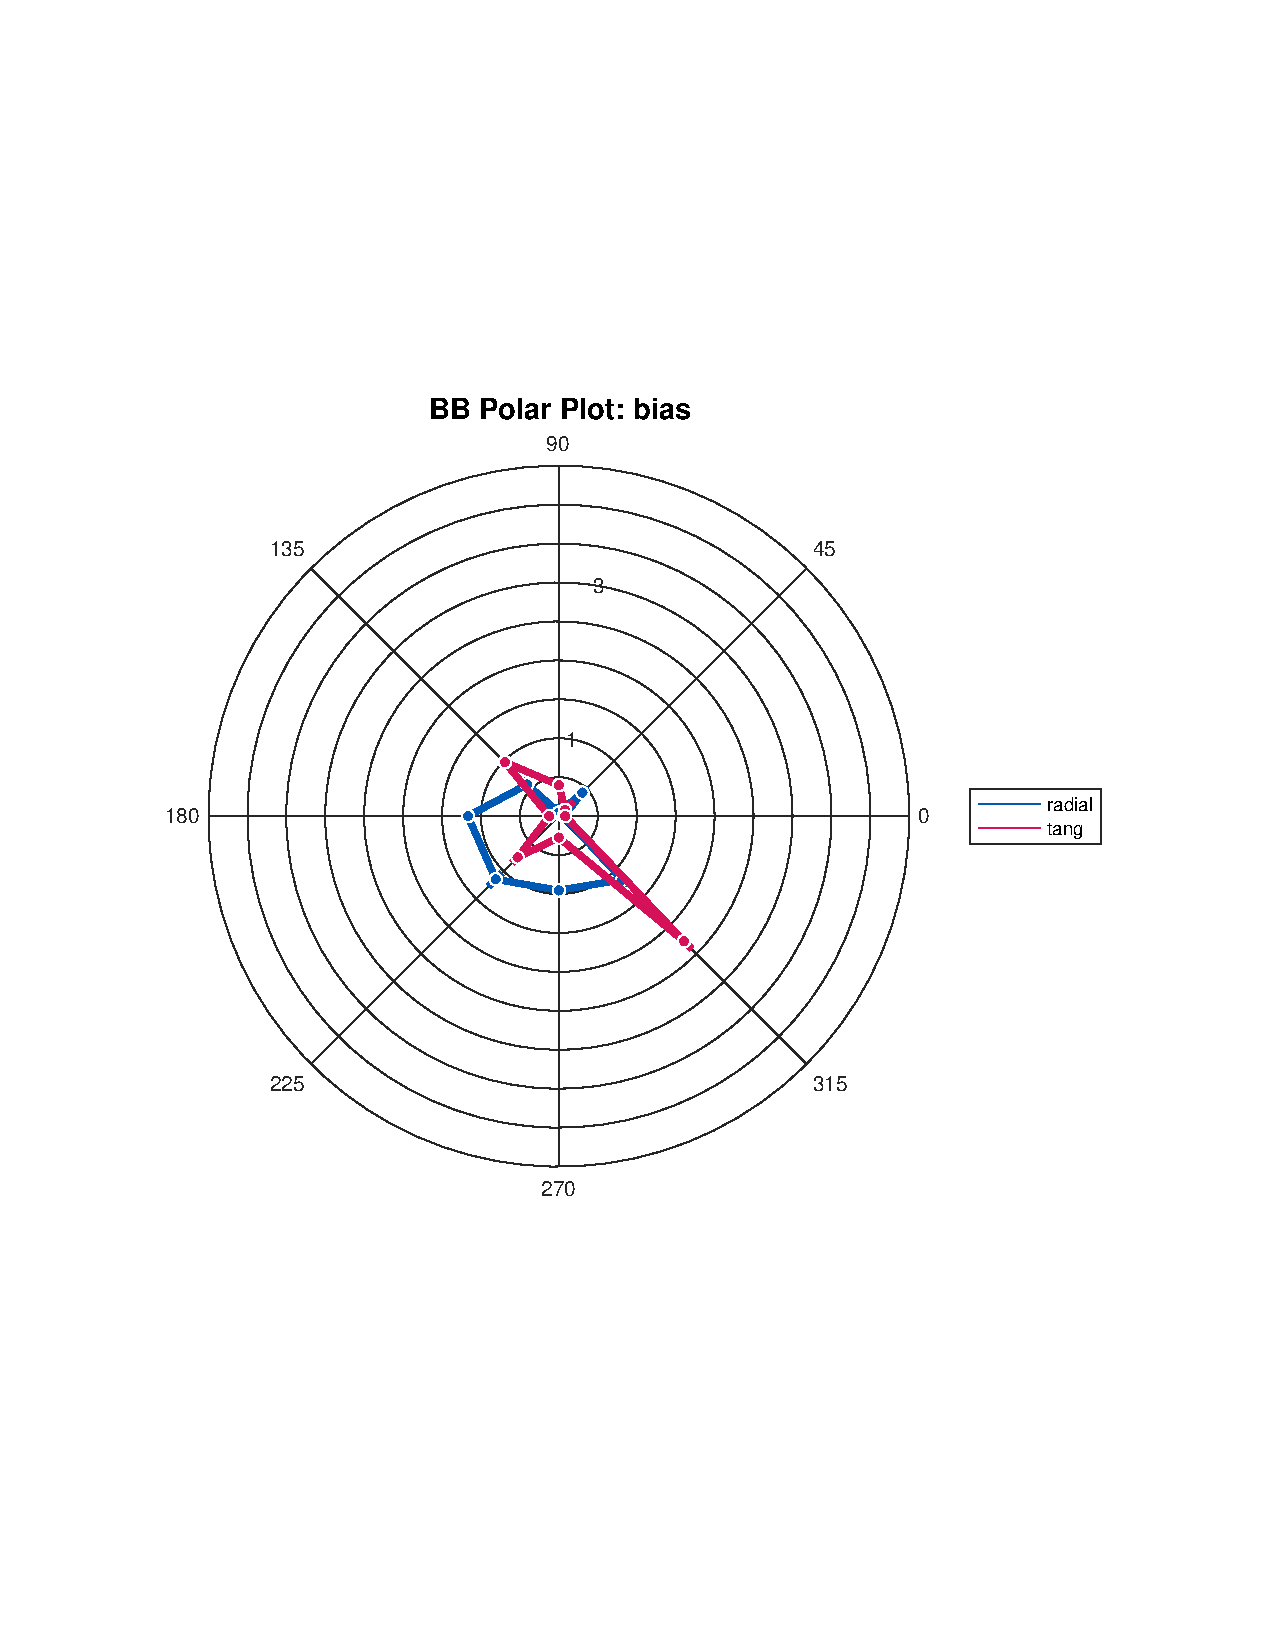
\includegraphics[scale=.3]{Images/BB_PP_bias_Alldata_2conds_relative.png}
\end{figure}
\begin{figure}[H]
\centering % centers the figure
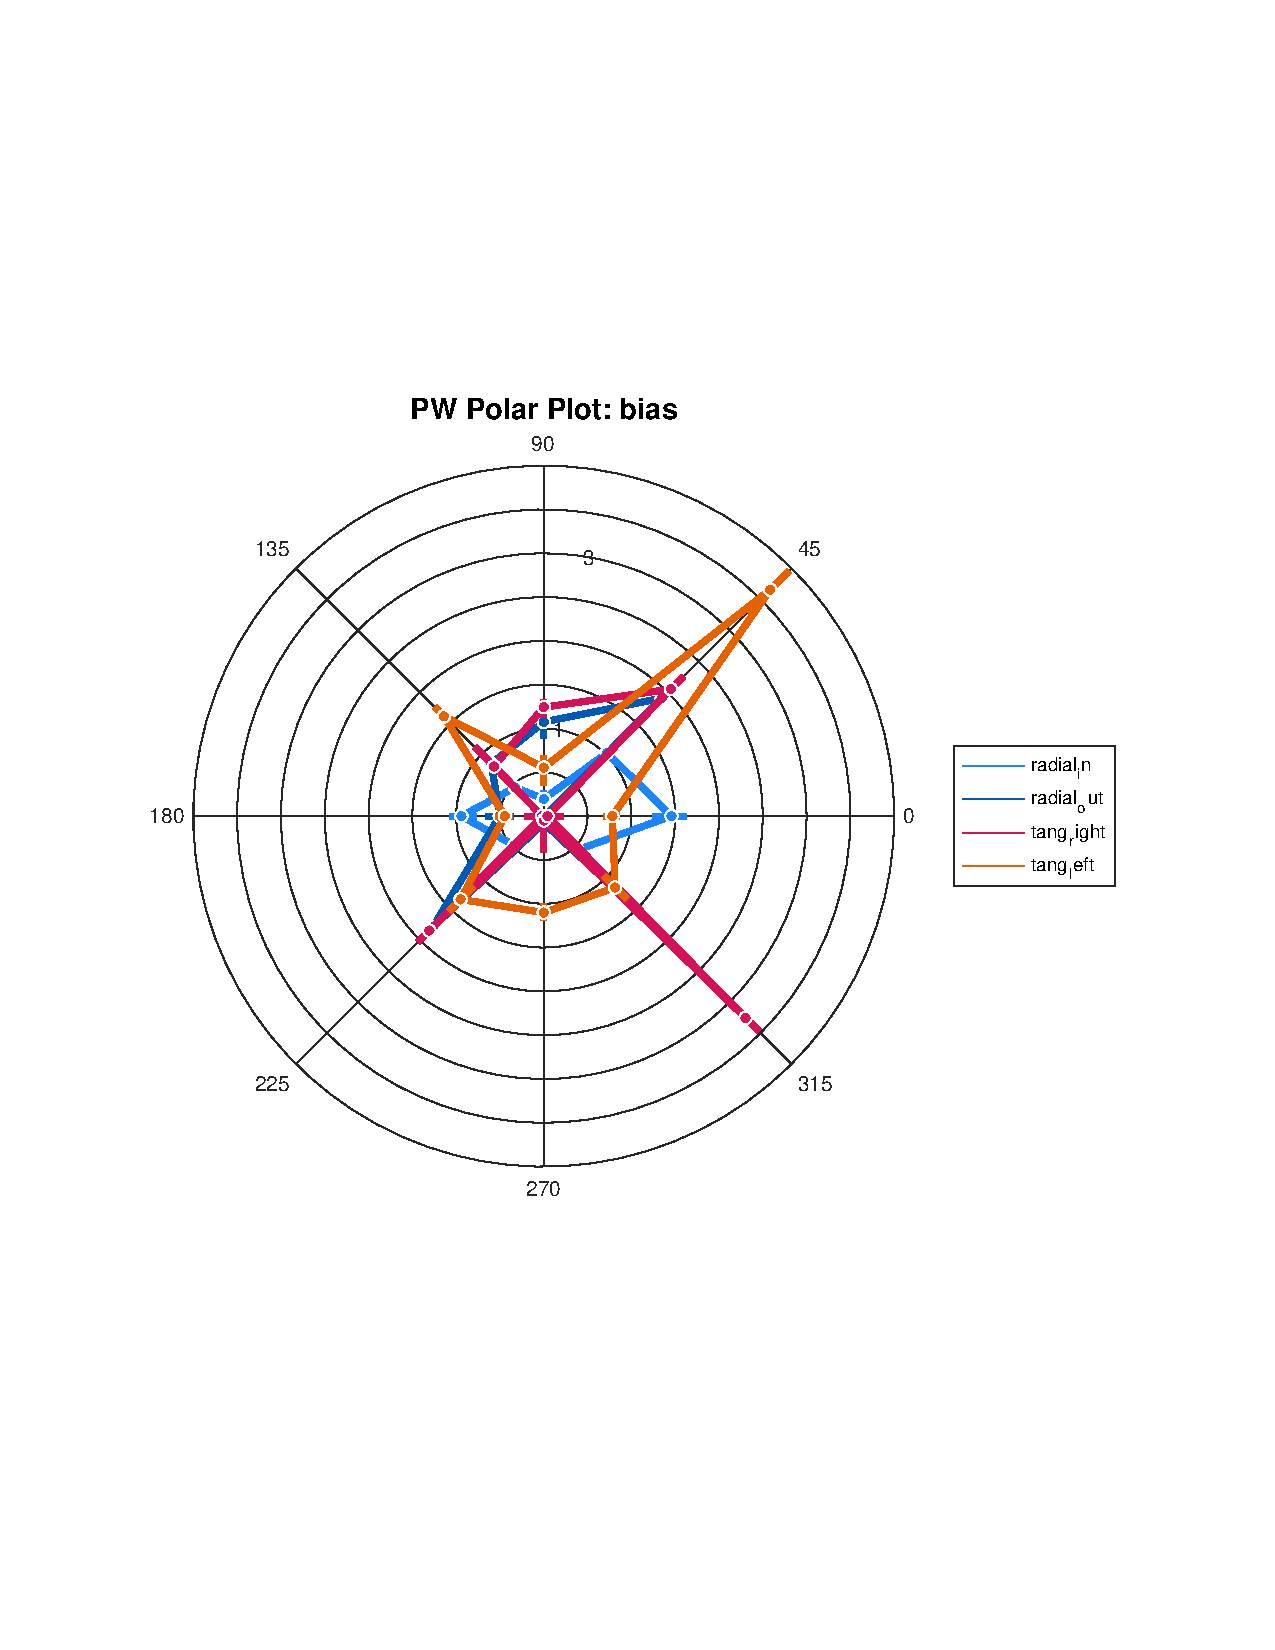
\includegraphics[scale=.3]{Images/PW_PP_bias_Alldata_4conds_relative.png}
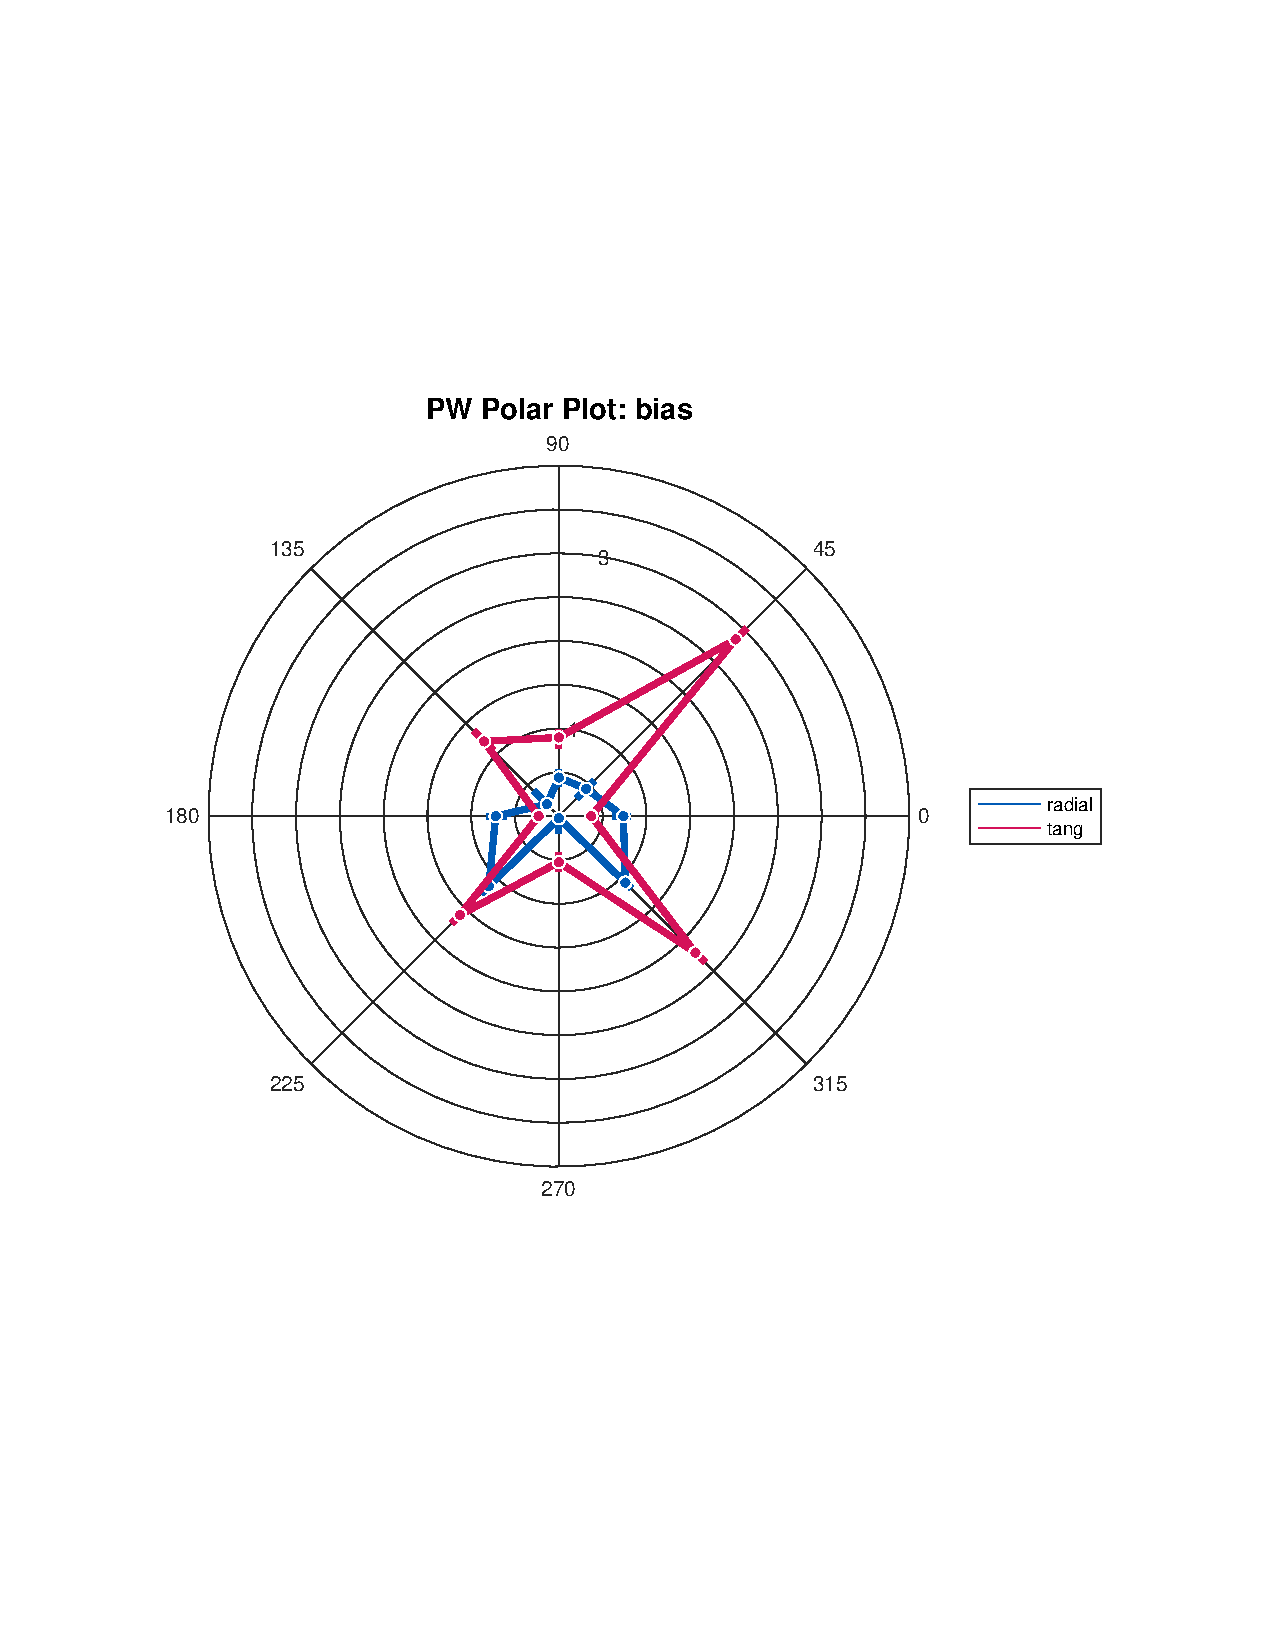
\includegraphics[scale=.3]{Images/PW_PP_bias_Alldata_2conds_relative.png}
\end{figure}
\begin{figure}[H]
\centering % centers the figure
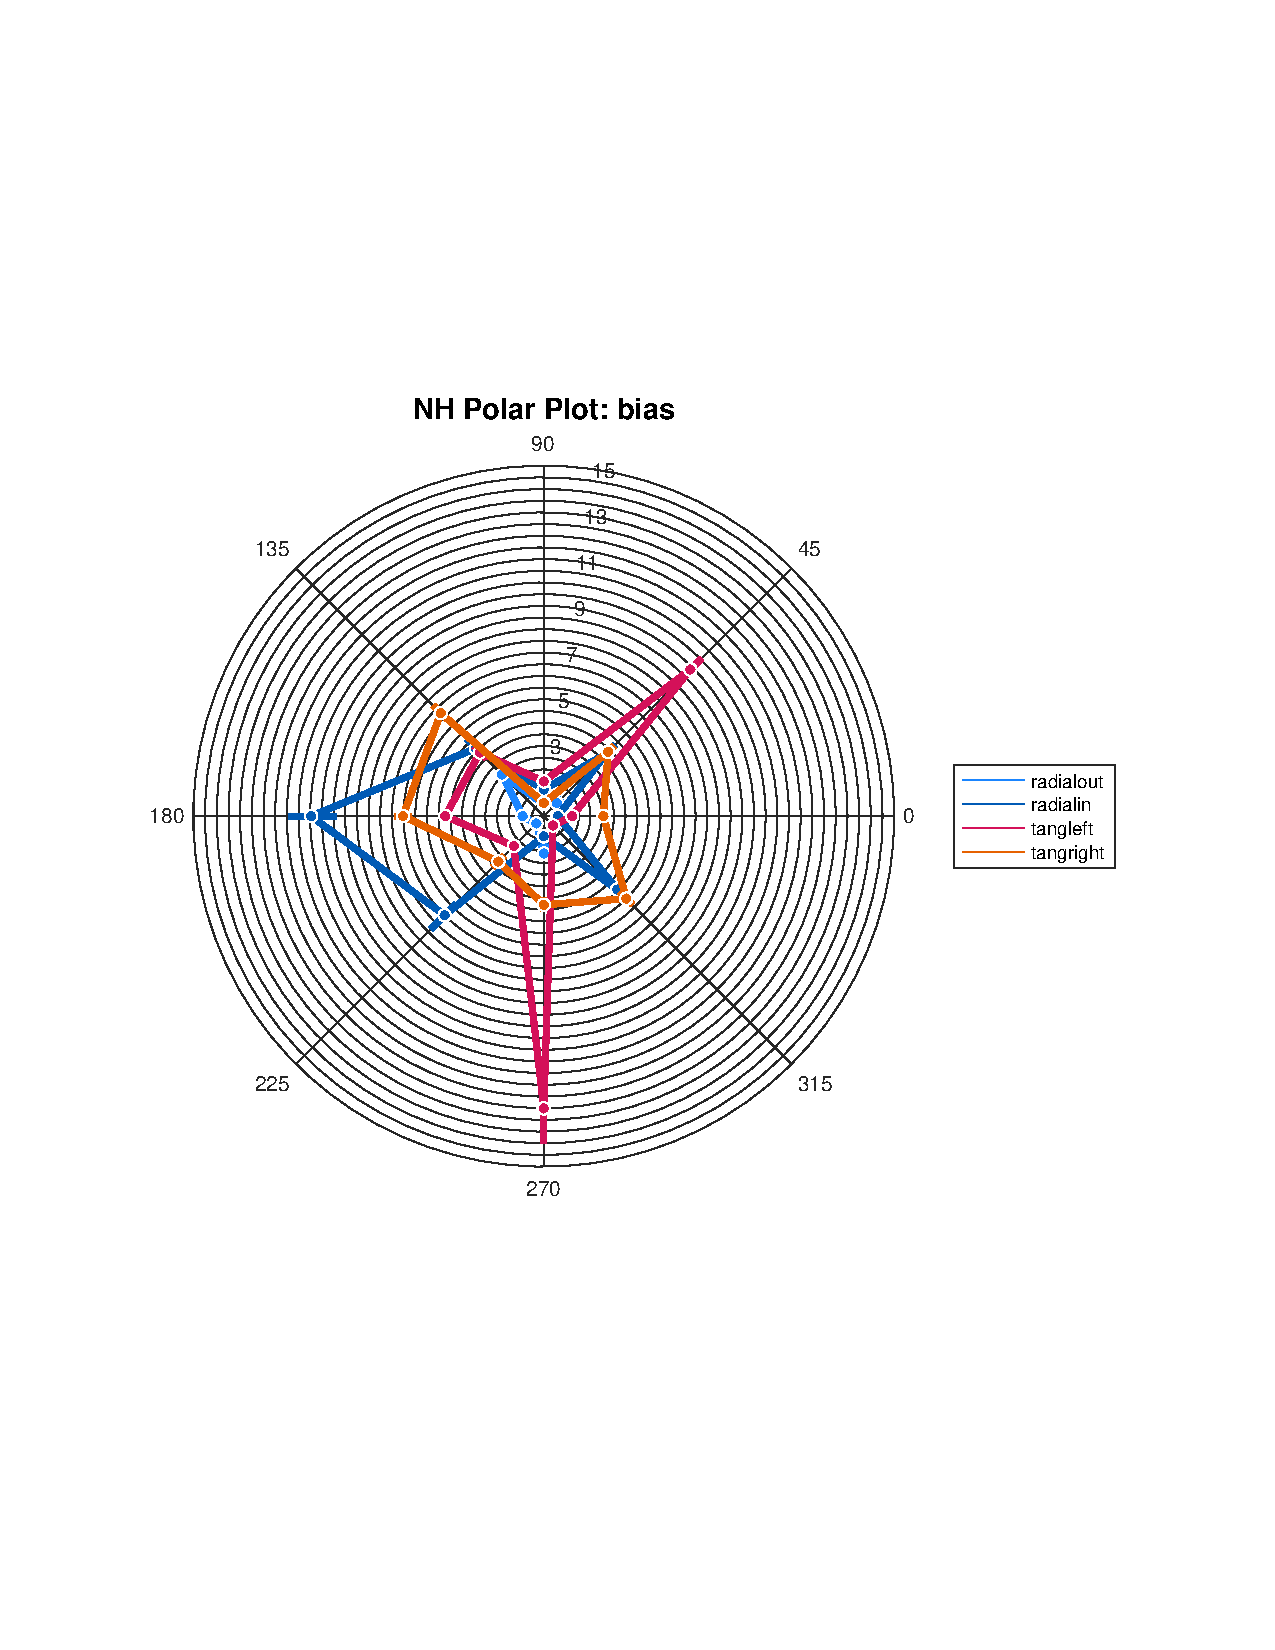
\includegraphics[scale=.3]{Images/NH_PP_bias_Alldata_4conds_relative.png}
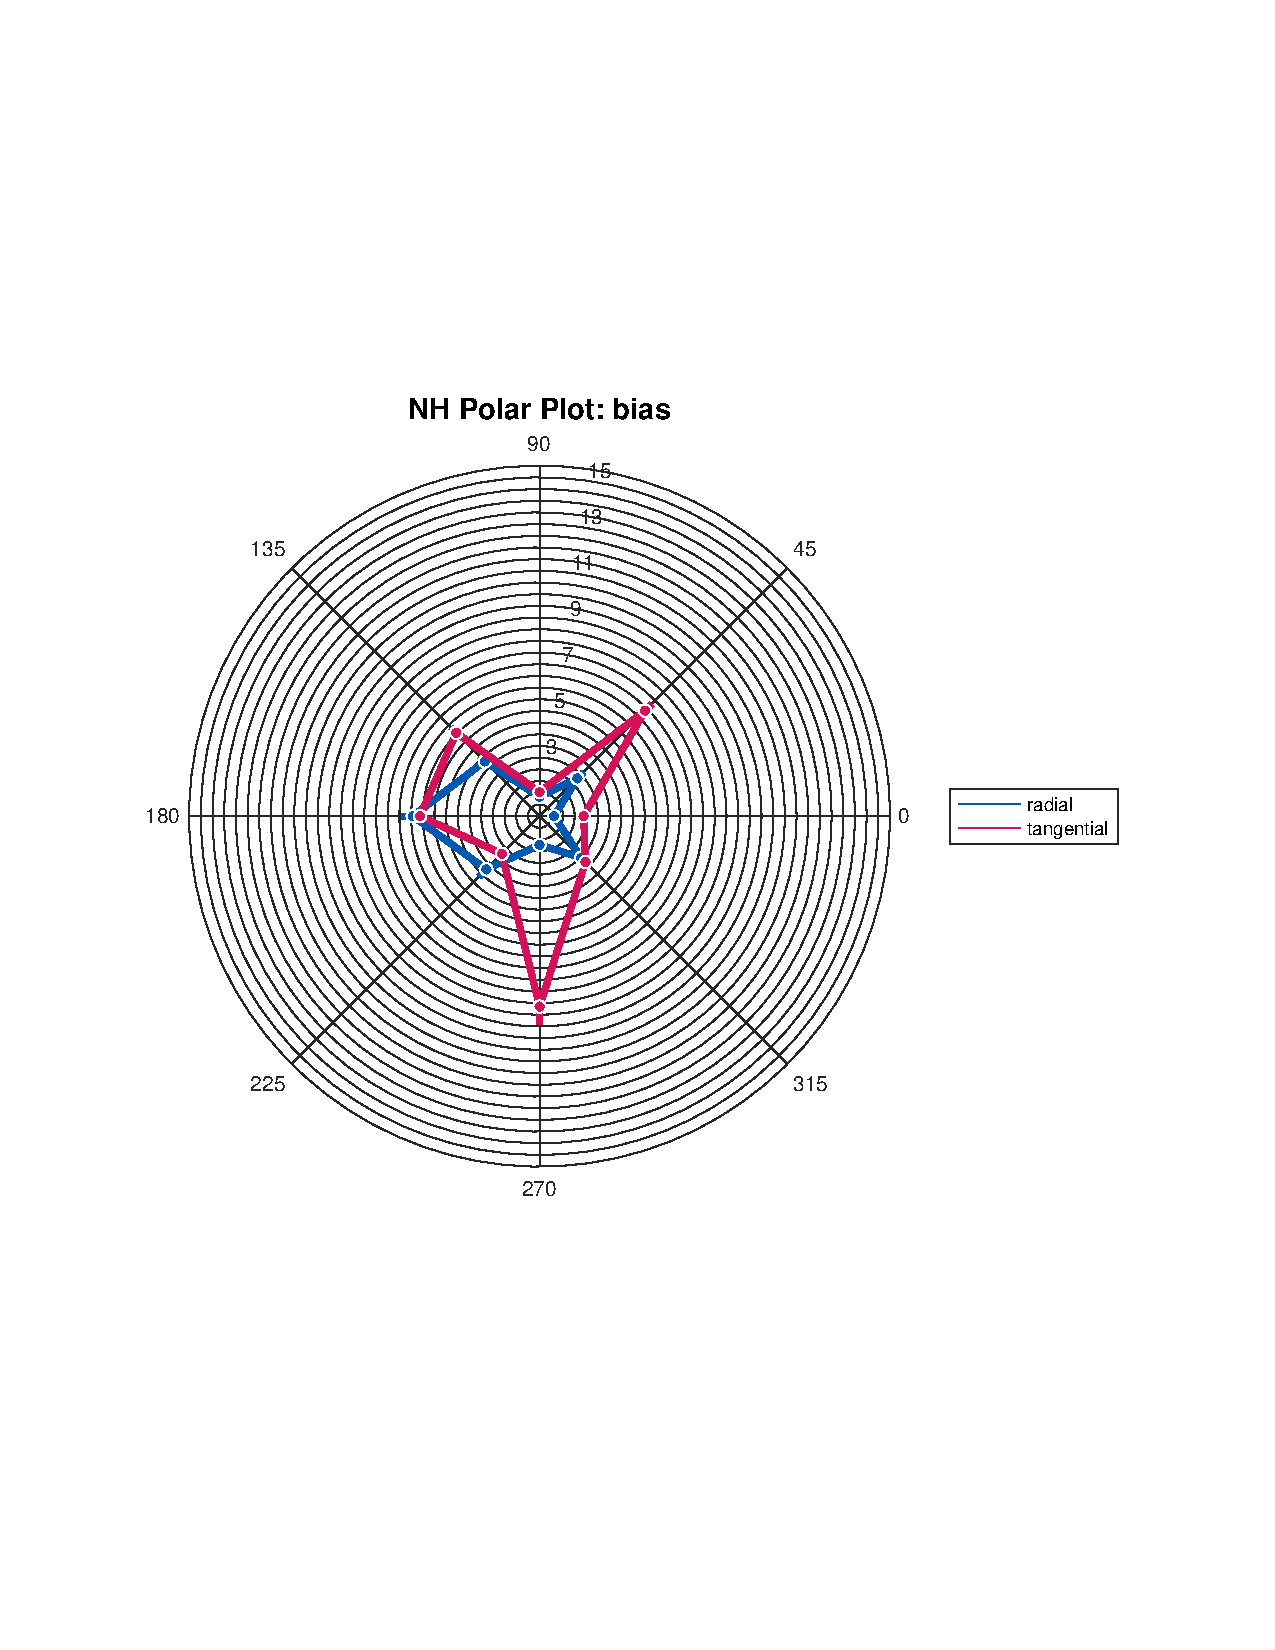
\includegraphics[scale=.3]{Images/NH_PP_bias_Alldata_2conds_relative.png}
\caption{LEFT: 200 trials per point. RIGHT: 400 trials per point. 68\% CI from 1000 bootstraps.}
\end{figure}

%\newpage
%\subsection{Bias Polar Plots (Absolute Value): Relative Motion}
%\begin{figure}[H]
%\centering % centers the figure
%\includegraphics[scale=.3]{Images/RE_PP_bias_abs_Alldata_4conds_relative.png}
%\includegraphics[scale=.3]{Images/RE_PP_bias_abs_Alldata_2conds_relative.png}
%\end{figure}
%\begin{figure}[H]
%\centering % centers the figure
%<<<<<<< HEAD
%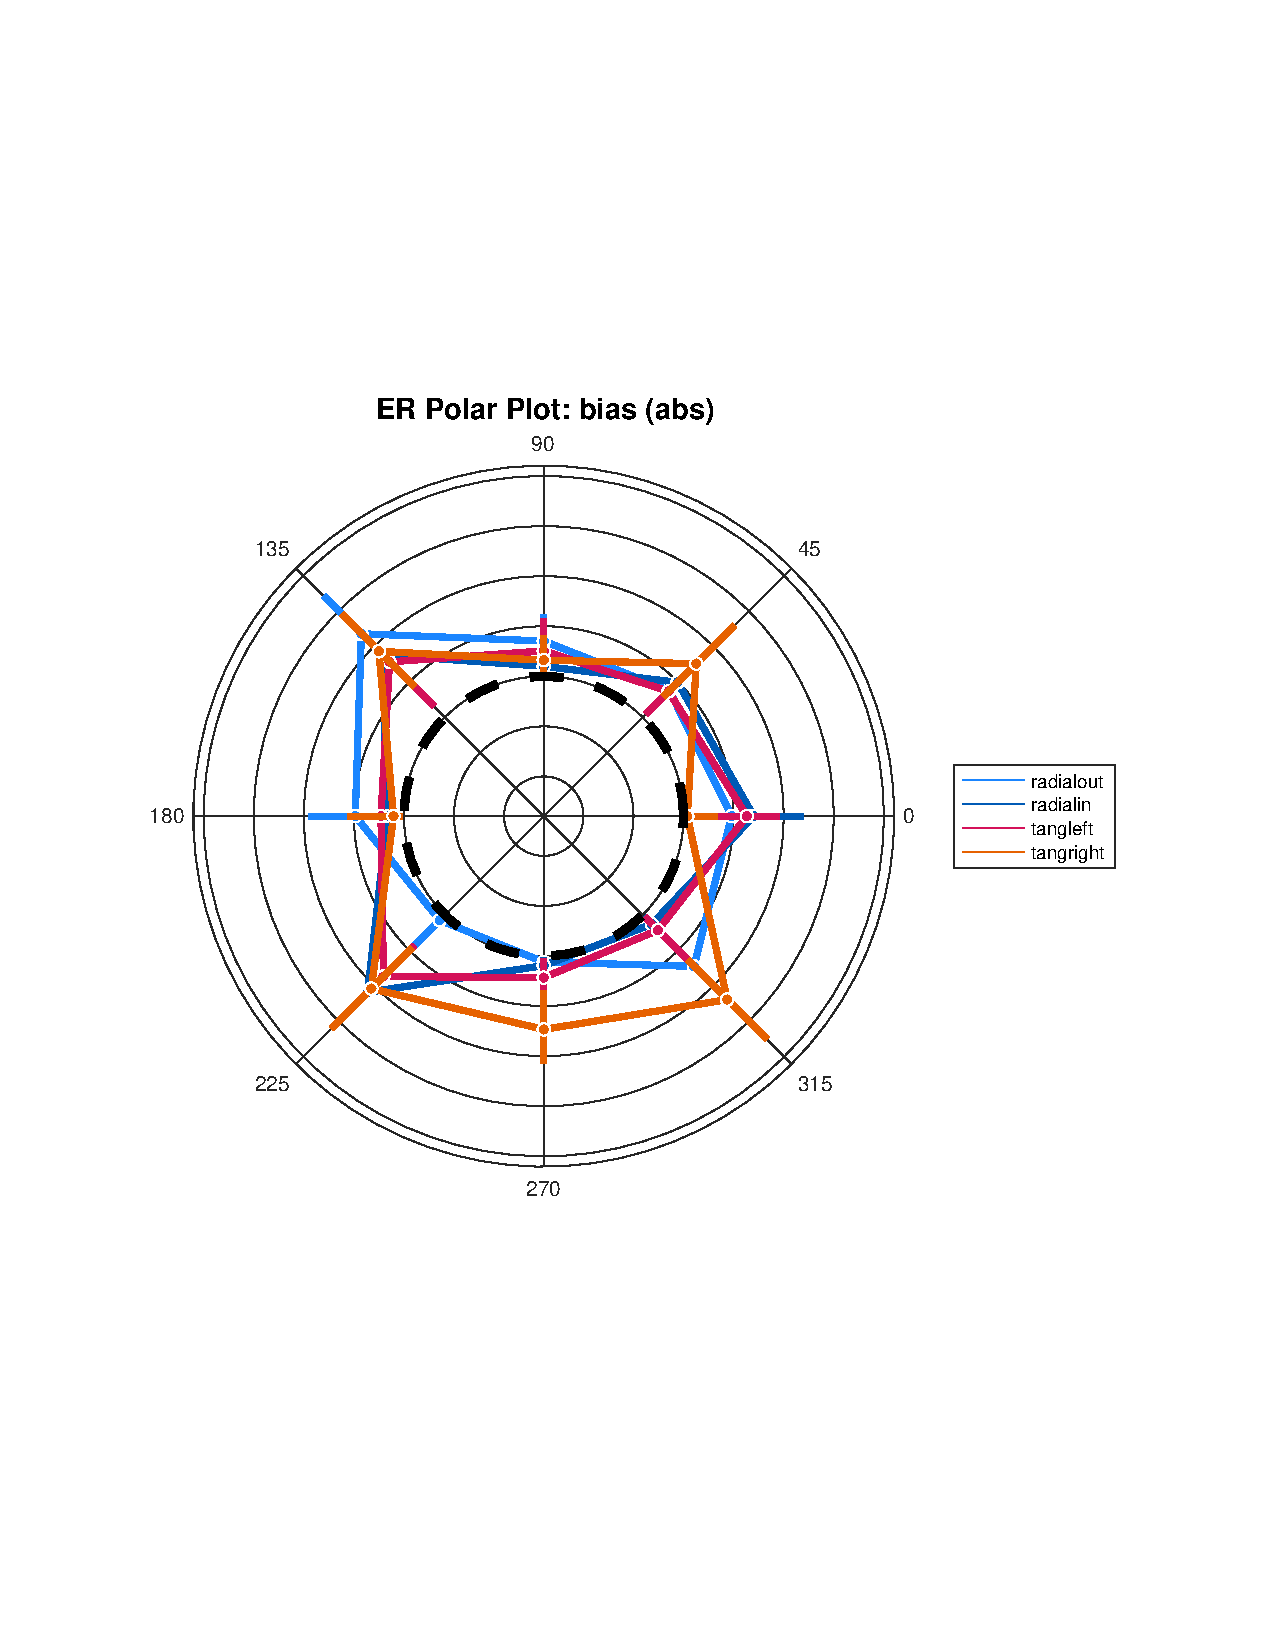
\includegraphics[scale=.3]{Images/ER_PP_bias_abs_Alldata_4conds_relative.png}
%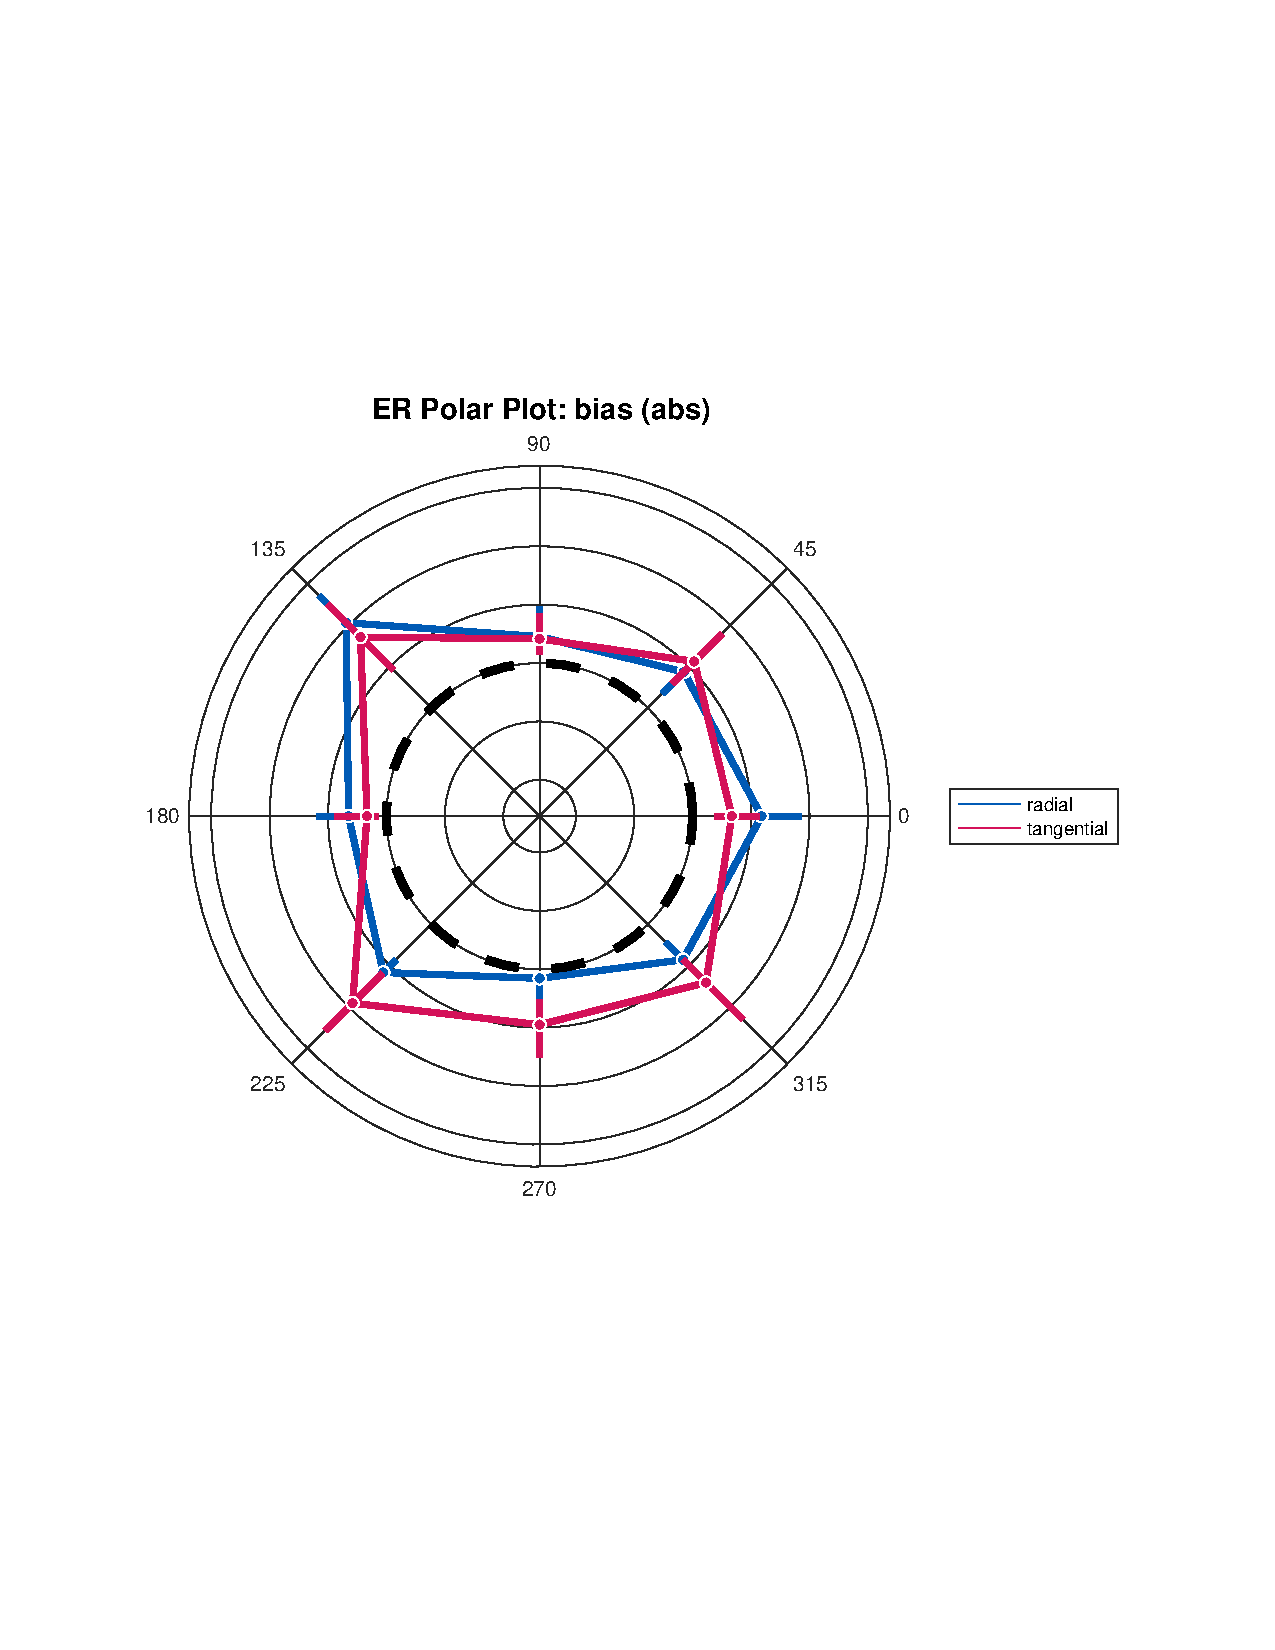
\includegraphics[scale=.3]{Images/ER_PP_bias_abs_Alldata_2conds_relative.png}
%\caption{Same subject (RE) but at half distance.}
%\end{figure}
%\begin{figure}[H]
%\centering % centers the figure
%\includegraphics[scale=.3]{Images/FH_PP_bias_abs_Alldata_4conds_relative.png}
%\includegraphics[scale=.3]{Images/FH_PP_bias_abs_Alldata_2conds_relative.png}
%\end{figure}
%\begin{figure}[H]
%\centering % centers the figure
%\includegraphics[scale=.3]{Images/BB_PP_bias_abs_Alldata_4conds_relative.png}
%\includegraphics[scale=.3]{Images/BB_PP_bias_abs_Alldata_2conds_relative.png}
%\end{figure}
%\begin{figure}[H]
%\centering % centers the figure
%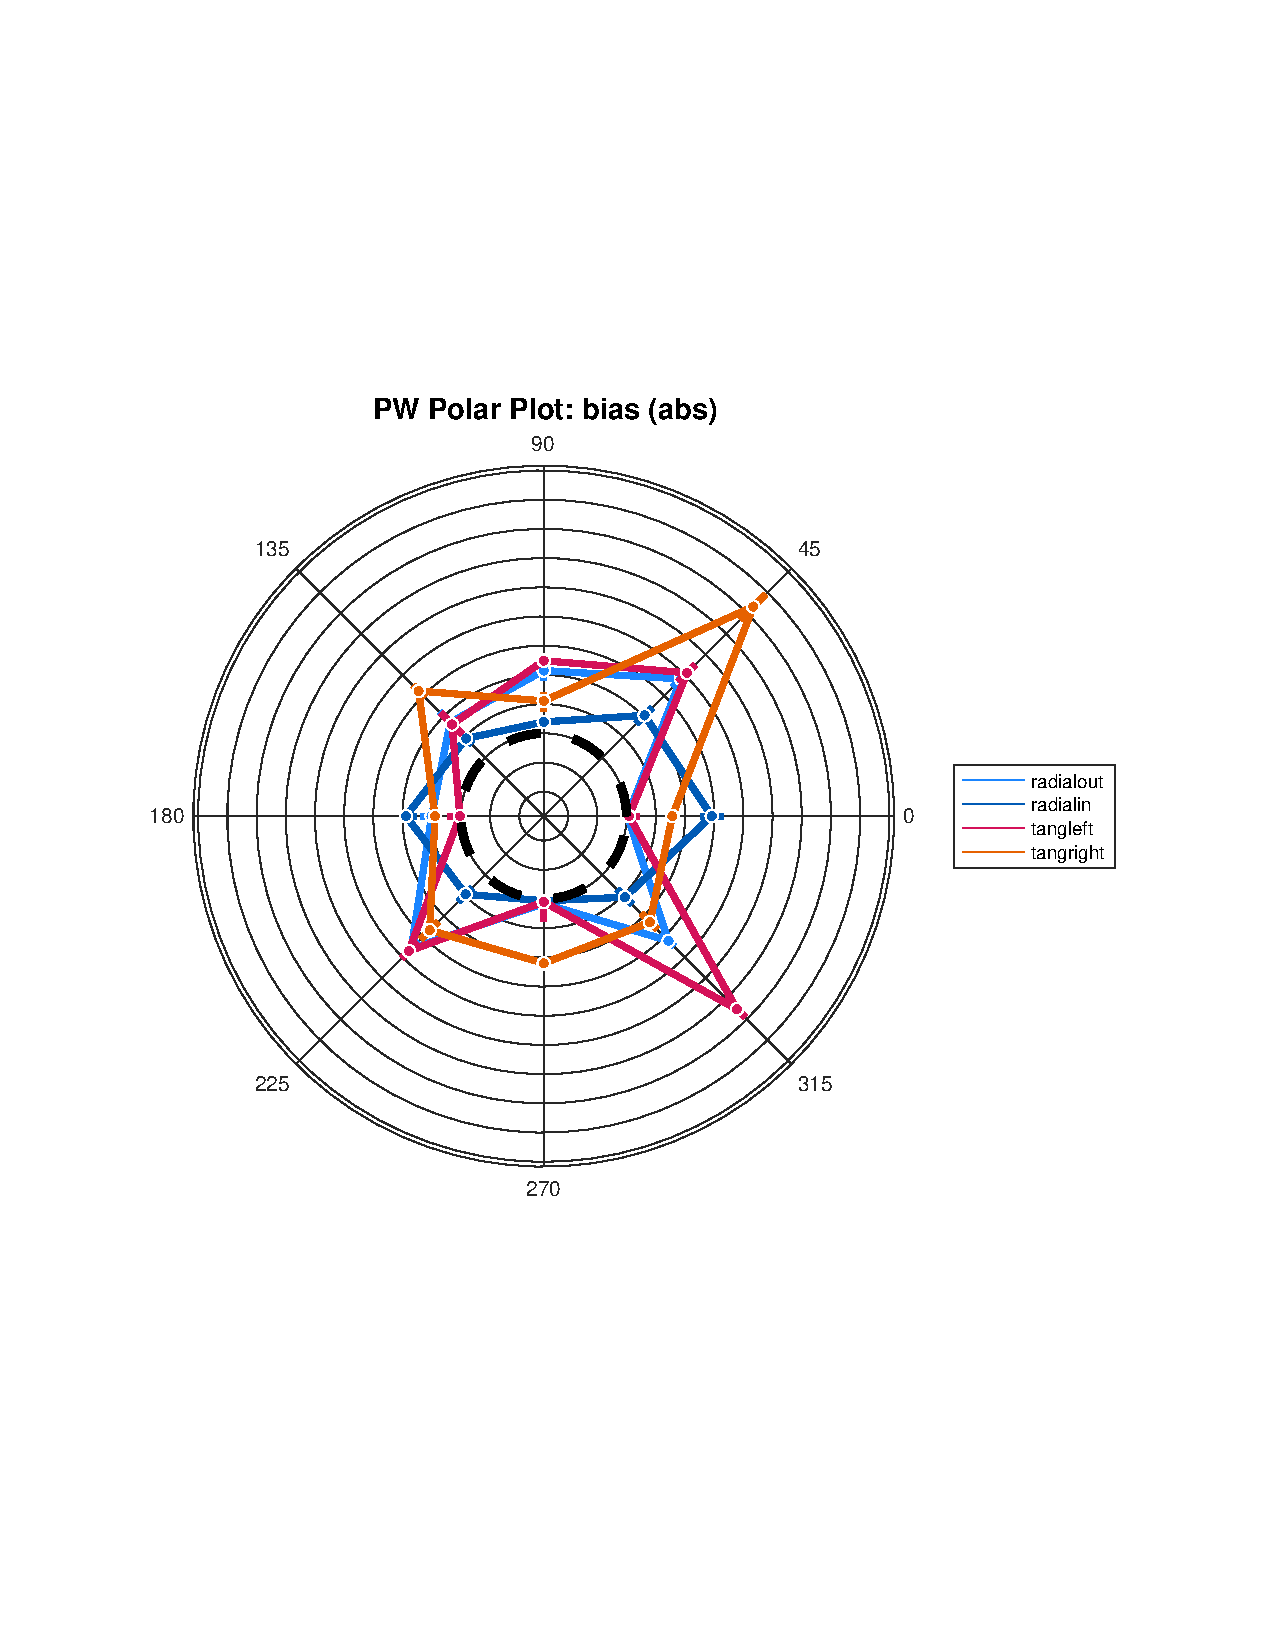
\includegraphics[scale=.3]{Images/PW_PP_bias_abs_Alldata_4conds_relative.png}
%\includegraphics[scale=.3]{Images/PW_PP_bias_abs_Alldata_2conds_relative.png}
%\end{figure}
%\begin{figure}[H]
%\centering % centers the figure
%\includegraphics[scale=.3]{Images/NH_PP_bias_abs_Alldata_4conds_relative.png}
%\includegraphics[scale=.3]{Images/NH_PP_bias_abs_Alldata_2conds_relative.png}
%\caption{LEFT: 200 trials per point. RIGHT: 400 trials per point. 95\% CI from 1000 bootstraps.}
%\end{figure}

\newpage
\section{Subject Data (Absolute motion)}
%\subsection{Sensitivity Polar Plots: Absolute Motion}
%\begin{figure}[H]
%\centering % centers the figure
%\includegraphics[scale=.3]{Images/RE_PP_sensitivity_Alldata_8conds_absolute.png}
%\includegraphics[scale=.3]{Images/ER_PP_sensitivity_Alldata_8conds_absolute.png}
%\includegraphics[scale=.3]{Images/FH_PP_sensitivity_Alldata_8conds_absolute.png}
%\includegraphics[scale=.3]{Images/BB_PP_sensitivity_Alldata_8conds_absolute.png}
%\includegraphics[scale=.3]{Images/PW_PP_sensitivity_Alldata_8conds_absolute.png}
%\includegraphics[scale=.3]{Images/NH_PP_sensitivity_Alldata_8conds_absolute.png}
%\caption{200 trials per point. 95\% CI from 1000 bootstraps.}
%\end{figure}
\subsection{Sensitivity Vector Plots: Absolute Motion}
\begin{figure}[H]
\centering % centers the figure
\includegraphics[scale=.3]{Images/RE_VP_Alldata_4conds_AbsoluteMotion.png}
\includegraphics[scale=.3]{Images/ER_VP_Alldata_4conds_AbsoluteMotion.png}
\includegraphics[scale=.3]{Images/FH_VP_Alldata_4conds_AbsoluteMotion.png}
\includegraphics[scale=.3]{Images/HF_VP_Alldata_4conds_AbsoluteMotion.png}
\includegraphics[scale=.3]{Images/BB_VP_Alldata_4conds_AbsoluteMotion.png}
\includegraphics[scale=.3]{Images/PW_VP_Alldata_4conds_AbsoluteMotion.png}
\includegraphics[scale=.3]{Images/NH_VP_Alldata_4conds_AbsoluteMotion.png}
\caption{Vector direction corresponds to direction of drift; magnitude corresponds to sensitivity.}
\end{figure}
%\subsection{Bias Polar Plots: Absolute Motion}
%\begin{figure}[H]
%\centering % centers the figure
%\includegraphics[scale=.3]{Images/RE_PP_bias_Alldata_8conds_absolute.png}
%\includegraphics[scale=.3]{Images/ER_PP_bias_Alldata_8conds_absolute.png}
%\includegraphics[scale=.3]{Images/FH_PP_bias_Alldata_8conds_absolute.png}
%\includegraphics[scale=.3]{Images/BB_PP_bias_Alldata_8conds_absolute.png}
%\includegraphics[scale=.3]{Images/PW_PP_bias_Alldata_8conds_absolute.png}
%\includegraphics[scale=.3]{Images/NH_PP_bias_Alldata_8conds_absolute.png}
%\caption{200 trials per point. 95\% CI from 1000 bootstraps.}
%\end{figure}
%\subsection{Bias Polar Plots (Absolute Value): Absolute Motion}
%\begin{figure}[H]
%\centering % centers the figure
%\includegraphics[scale=.3]{Images/RE_PP_bias_abs_Alldata_8conds_absolute.png}
%<<<<<<< HEAD
%\includegraphics[scale=.3]{Images/ER_PP_bias_abs_Alldata_8conds_absolute.png}
%=======
%>>>>>>> 34c5efb959d1a380cfdb3aacb5661b6c2ac21558
%\includegraphics[scale=.3]{Images/FH_PP_bias_abs_Alldata_8conds_absolute.png}
%\includegraphics[scale=.3]{Images/BB_PP_bias_abs_Alldata_8conds_absolute.png}
%\includegraphics[scale=.3]{Images/PW_PP_bias_abs_Alldata_8conds_absolute.png}
%\includegraphics[scale=.3]{Images/NH_PP_bias_abs_Alldata_8conds_absolute.png}
%\caption{200 trials per point. 95\% CI from 1000 bootstraps.}
%\end{figure}

\newpage
\section{Group Data (Relative motion)}
\subsection{Sensitivity Polar Plots: Relative Motion}
\begin{figure}[H]
\centering % centers the figure
\includegraphics[scale=.35]{Images/ALLSUBJ_PP_sensitivity_Alldata_4conds_relative.png}
\includegraphics[scale=.35]{Images/ALLSUBJ_PP_sensitivity_Alldata_2conds_relative.png}
\caption{LEFT: 600 trials per point. RIGHT: Each point is 1200 trials. Error bars represent SEM across subjects.}
\end{figure}
\subsection{Z-score Sensitivity Polar Plots: Relative Motion}
\begin{figure}[H]
\centering % centers the figure
\includegraphics[scale=.35]{Images/ALLSUBJ_PP_z-score sensitivity_Alldata_4conds_relative.png}
\includegraphics[scale=.35]{Images/ALLSUBJ_PP_z-score sensitivity_Alldata_2conds_relative.png}
\caption{LEFT: 600 trials per point. RIGHT: Each point is 1200 trials. Error bars represent SEM across subject z-scores.}
\end{figure}
\subsection{Bias (Abs) Polar Plots: Relative Motion}
\begin{figure}[H]
\centering % centers the figure
\includegraphics[scale=.35]{Images/ALLSUBJ_PP_bias_Alldata_4conds_relative.png}
\includegraphics[scale=.35]{Images/ALLSUBJ_PP_bias_Alldata_2conds_relative.png}
\end{figure}
\subsection{Z-score Bias Polar Plots: Relative Motion}
\begin{figure}[H]
\centering % centers the figure
\includegraphics[scale=.35]{Images/ALLSUBJ_PP_z-score bias_Alldata_4conds_relative.png}
\includegraphics[scale=.35]{Images/ALLSUBJ_PP_z-score bias_Alldata_2conds_relative.png}
\caption{I think these aren't useful since the dashed line no longer indicates no bias (just mean).}
\end{figure}
%\subsection{Bias Polar Plots (Absolute Value): Relative Motion}
%\begin{figure}[H]
%\centering % centers the figure
%\includegraphics[scale=.35]{Images/ALLSUBJ_PP_bias_abs_Alldata_4conds_relative.png}
%\includegraphics[scale=.35]{Images/ALLSUBJ_PP_bias_abs_Alldata_2conds_relative.png}
%\end{figure}
%\subsection{Z-score Bias Polar Plots (Absolute Value): Relative Motion}
%\begin{figure}[H]
%\centering % centers the figure
%\includegraphics[scale=.35]{Images/ALLSUBJ_PP_z-score bias_abs_Alldata_4conds_relative.png}
%\includegraphics[scale=.35]{Images/ALLSUBJ_PP_z-score bias_abs_Alldata_2conds_relative.png}
%\caption{I think these aren't useful since the dashed line no longer indicates no bias (just mean).}
%\end{figure}

\newpage
\section{Group Data (Absolute motion)}
\subsection{Sensitivity Polar Plots: Absolute Motion}
\begin{figure}[H]
\centering % centers the figure
\includegraphics[scale=.35]{Images/ALLSUBJ_PP_sensitivity_Alldata_8conds_absolute.png}
\includegraphics[scale=.35]{Images/ALLSUBJ_VP_Alldata_4conds_AbsoluteMotion.png}
\caption{LEFT: Polar plots of average sensitivity, CIs represent SEM. RIGHT: Vector plots of average sensitivity.}
\end{figure}
\subsection{Bias Polar Plots: Absolute Motion}
\begin{figure}[H]
\centering % centers the figure
\includegraphics[scale=.35]{Images/ALLSUBJ_PP_bias_Alldata_8conds_absolute.png}
\includegraphics[scale=.35]{Images/ALLSUBJ_PP_bias_abs_Alldata_8conds_absolute.png}
\caption{LEFT: Polar plots of bias. RIGHT: Polar plots of average abs(bias).}
\end{figure}

\newpage
\section{Supplementary Images: PFs per location}
\subsection{RE PFs Per Location}
\begin{figure}[H]
\centering % centers the figure
\includegraphics[scale=.15]{Images/RE_PF_loc0_4conds.png}
\includegraphics[scale=.15]{Images/RE_PF_loc0_2conds.png}
\end{figure}
\begin{figure}[H]
\centering % centers the figure
\includegraphics[scale=.15]{Images/RE_PF_loc45_4conds.png}
\includegraphics[scale=.15]{Images/RE_PF_loc45_2conds.png}
\end{figure}
\begin{figure}[H]
\centering % centers the figure
\includegraphics[scale=.15]{Images/RE_PF_loc90_4conds.png}
\includegraphics[scale=.15]{Images/RE_PF_loc90_2conds.png}
\end{figure}
\begin{figure}[H]
\centering % centers the figure
\includegraphics[scale=.15]{Images/RE_PF_loc135_4conds.png}
\includegraphics[scale=.15]{Images/RE_PF_loc135_2conds.png}
\end{figure}
\begin{figure}[H]
\centering % centers the figure
\includegraphics[scale=.15]{Images/RE_PF_loc180_4conds.png}
\includegraphics[scale=.15]{Images/RE_PF_loc180_2conds.png}
\end{figure}
\begin{figure}[H]
\centering % centers the figure
\includegraphics[scale=.15]{Images/RE_PF_loc225_4conds.png}
\includegraphics[scale=.15]{Images/RE_PF_loc225_2conds.png}
\end{figure}
\begin{figure}[H]
\centering % centers the figure
\includegraphics[scale=.15]{Images/RE_PF_loc270_4conds.png}
\includegraphics[scale=.15]{Images/RE_PF_loc270_2conds.png}
\end{figure}
\begin{figure}[H]
\centering % centers the figure
\includegraphics[scale=.15]{Images/RE_PF_loc315_4conds.png}
\includegraphics[scale=.15]{Images/RE_PF_loc315_2conds.png}
\end{figure}

\newpage
\subsection{FH PFs Per Location}
\begin{figure}[H]
\centering % centers the figure
\includegraphics[scale=.15]{Images/FH_PF_loc0_4conds.png}
\includegraphics[scale=.15]{Images/FH_PF_loc0_2conds.png}
\end{figure}
\begin{figure}[H]
\centering % centers the figure
\includegraphics[scale=.15]{Images/FH_PF_loc45_4conds.png}
\includegraphics[scale=.15]{Images/FH_PF_loc45_2conds.png}
\end{figure}
\begin{figure}[H]
\centering % centers the figure
\includegraphics[scale=.15]{Images/FH_PF_loc90_4conds.png}
\includegraphics[scale=.15]{Images/FH_PF_loc90_2conds.png}
\end{figure}
\begin{figure}[H]
\centering % centers the figure
\includegraphics[scale=.15]{Images/FH_PF_loc135_4conds.png}
\includegraphics[scale=.15]{Images/FH_PF_loc135_2conds.png}
\end{figure}
\begin{figure}[H]
\centering % centers the figure
\includegraphics[scale=.15]{Images/FH_PF_loc180_4conds.png}
\includegraphics[scale=.15]{Images/FH_PF_loc180_2conds.png}
\end{figure}
\begin{figure}[H]
\centering % centers the figure
\includegraphics[scale=.15]{Images/FH_PF_loc225_4conds.png}
\includegraphics[scale=.15]{Images/FH_PF_loc225_2conds.png}
\end{figure}
\begin{figure}[H]
\centering % centers the figure
\includegraphics[scale=.15]{Images/FH_PF_loc270_4conds.png}
\includegraphics[scale=.15]{Images/FH_PF_loc270_2conds.png}
\end{figure}
\begin{figure}[H]
\centering % centers the figure
\includegraphics[scale=.15]{Images/FH_PF_loc315_4conds.png}
\includegraphics[scale=.15]{Images/FH_PF_loc315_2conds.png}
\end{figure}

\newpage
\subsection{BB PFs Per Location}
\begin{figure}[H]
\centering % centers the figure
\includegraphics[scale=.15]{Images/BB_PF_loc0_4conds.png}
\includegraphics[scale=.15]{Images/BB_PF_loc0_2conds.png}
\end{figure}
\begin{figure}[H]
\centering % centers the figure
\includegraphics[scale=.15]{Images/BB_PF_loc45_4conds.png}
\includegraphics[scale=.15]{Images/BB_PF_loc45_2conds.png}
\end{figure}
\begin{figure}[H]
\centering % centers the figure
\includegraphics[scale=.15]{Images/BB_PF_loc90_4conds.png}
\includegraphics[scale=.15]{Images/BB_PF_loc90_2conds.png}
\end{figure}
\begin{figure}[H]
\centering % centers the figure
\includegraphics[scale=.15]{Images/BB_PF_loc135_4conds.png}
\includegraphics[scale=.15]{Images/BB_PF_loc135_2conds.png}
\end{figure}
\begin{figure}[H]
\centering % centers the figure
\includegraphics[scale=.15]{Images/BB_PF_loc180_4conds.png}
\includegraphics[scale=.15]{Images/BB_PF_loc180_2conds.png}
\end{figure}
\begin{figure}[H]
\centering % centers the figure
\includegraphics[scale=.15]{Images/BB_PF_loc225_4conds.png}
\includegraphics[scale=.15]{Images/BB_PF_loc225_2conds.png}
\end{figure}
\begin{figure}[H]
\centering % centers the figure
\includegraphics[scale=.15]{Images/BB_PF_loc270_4conds.png}
\includegraphics[scale=.15]{Images/BB_PF_loc270_2conds.png}
\end{figure}
\begin{figure}[H]
\centering % centers the figure
\includegraphics[scale=.15]{Images/BB_PF_loc315_4conds.png}
\includegraphics[scale=.15]{Images/BB_PF_loc315_2conds.png}
\end{figure}

\newpage
\subsection{PW PFs Per Location}
\begin{figure}[H]
\centering % centers the figure
\includegraphics[scale=.15]{Images/PW_PF_loc0_4conds.png}
\includegraphics[scale=.15]{Images/PW_PF_loc0_2conds.png}
\end{figure}
\begin{figure}[H]
\centering % centers the figure
\includegraphics[scale=.15]{Images/PW_PF_loc45_4conds.png}
\includegraphics[scale=.15]{Images/PW_PF_loc45_2conds.png}
\end{figure}
\begin{figure}[H]
\centering % centers the figure
\includegraphics[scale=.15]{Images/PW_PF_loc90_4conds.png}
\includegraphics[scale=.15]{Images/PW_PF_loc90_2conds.png}
\end{figure}
\begin{figure}[H]
\centering % centers the figure
\includegraphics[scale=.15]{Images/PW_PF_loc135_4conds.png}
\includegraphics[scale=.15]{Images/PW_PF_loc135_2conds.png}
\end{figure}
\begin{figure}[H]
\centering % centers the figure
\includegraphics[scale=.15]{Images/PW_PF_loc180_4conds.png}
\includegraphics[scale=.15]{Images/PW_PF_loc180_2conds.png}
\end{figure}
\begin{figure}[H]
\centering % centers the figure
\includegraphics[scale=.15]{Images/PW_PF_loc225_4conds.png}
\includegraphics[scale=.15]{Images/PW_PF_loc225_2conds.png}
\end{figure}
\begin{figure}[H]
\centering % centers the figure
\includegraphics[scale=.15]{Images/PW_PF_loc270_4conds.png}
\includegraphics[scale=.15]{Images/PW_PF_loc270_2conds.png}
\end{figure}
\begin{figure}[H]
\centering % centers the figure
\includegraphics[scale=.15]{Images/PW_PF_loc315_4conds.png}
\includegraphics[scale=.15]{Images/PW_PF_loc315_2conds.png}
\end{figure}

\newpage
\subsection{NH PFs Per Location}
\begin{figure}[H]
\centering % centers the figure
\includegraphics[scale=.15]{Images/NH_PF_loc0_4conds.png}
\includegraphics[scale=.15]{Images/NH_PF_loc0_2conds.png}
\end{figure}
\begin{figure}[H]
\centering % centers the figure
\includegraphics[scale=.15]{Images/NH_PF_loc45_4conds.png}
\includegraphics[scale=.15]{Images/NH_PF_loc45_2conds.png}
\end{figure}
\begin{figure}[H]
\centering % centers the figure
\includegraphics[scale=.15]{Images/NH_PF_loc90_4conds.png}
\includegraphics[scale=.15]{Images/NH_PF_loc90_2conds.png}
\end{figure}
\begin{figure}[H]
\centering % centers the figure
\includegraphics[scale=.15]{Images/NH_PF_loc135_4conds.png}
\includegraphics[scale=.15]{Images/NH_PF_loc135_2conds.png}
\end{figure}
\begin{figure}[H]
\centering % centers the figure
\includegraphics[scale=.15]{Images/NH_PF_loc180_4conds.png}
\includegraphics[scale=.15]{Images/NH_PF_loc180_2conds.png}
\end{figure}
\begin{figure}[H]
\centering % centers the figure
\includegraphics[scale=.15]{Images/NH_PF_loc225_4conds.png}
\includegraphics[scale=.15]{Images/NH_PF_loc225_2conds.png}
\end{figure}
\begin{figure}[H]
\centering % centers the figure
\includegraphics[scale=.15]{Images/NH_PF_loc270_4conds.png}
\includegraphics[scale=.15]{Images/NH_PF_loc270_2conds.png}
\end{figure}
\begin{figure}[H]
\centering % centers the figure
\includegraphics[scale=.15]{Images/NH_PF_loc315_4conds.png}
\includegraphics[scale=.15]{Images/NH_PF_loc315_2conds.png}
\end{figure}

\newpage
\section{Supplementary Images: Subject Cartesian Line Plots} 
\subsection{Sensitivity Cartesian Line Plots: Relative Motion}
\begin{figure}[H]
\centering % centers the figure
\includegraphics[scale=.3]{Images/RE_LP_sensitivity_Alldata_4conds.png}
\includegraphics[scale=.3]{Images/RE_LP_sensitivity_Alldata_2conds.png}
\end{figure}
\begin{figure}[H]
\centering % centers the figure
\includegraphics[scale=.3]{Images/FH_LP_sensitivity_Alldata_4conds.png}
\includegraphics[scale=.3]{Images/FH_LP_sensitivity_Alldata_2conds.png}
\end{figure}
\begin{figure}[H]
\centering % centers the figure
\includegraphics[scale=.3]{Images/BB_LP_sensitivity_Alldata_4conds.png}
\includegraphics[scale=.3]{Images/BB_LP_sensitivity_Alldata_2conds.png}
\end{figure}
\begin{figure}[H]
\centering % centers the figure
\includegraphics[scale=.3]{Images/PW_LP_sensitivity_Alldata_4conds_relative.png}
\includegraphics[scale=.3]{Images/PW_LP_sensitivity_Alldata_2conds_relative.png}
\end{figure}
\begin{figure}[H]
\centering % centers the figure
\includegraphics[scale=.3]{Images/NH_LP_sensitivity_Alldata_4conds_relative.png}
\includegraphics[scale=.3]{Images/NH_LP_sensitivity_Alldata_2conds_relative.png}
\caption{LEFT: 200 trials per point. RIGHT: 400 trials per point. 95\% CI from 1000 bootstraps.}
\end{figure}
\subsection{Bias Cartesian Line Plots: Relative Motion}
\begin{figure}[H]
\centering % centers the figure
\includegraphics[scale=.3]{Images/RE_LP_bias_Alldata_4conds.png}
\includegraphics[scale=.3]{Images/RE_LP_bias_Alldata_2conds.png}
\end{figure}
\begin{figure}[H]
\centering % centers the figure
\includegraphics[scale=.3]{Images/FH_LP_bias_Alldata_4conds.png}
\includegraphics[scale=.3]{Images/FH_LP_bias_Alldata_2conds.png}
\end{figure}
\begin{figure}[H]
\centering % centers the figure
\includegraphics[scale=.3]{Images/BB_LP_bias_Alldata_4conds.png}
\includegraphics[scale=.3]{Images/BB_LP_bias_Alldata_2conds.png}
\end{figure}
\begin{figure}[H]
\centering % centers the figure
\includegraphics[scale=.3]{Images/PW_LP_bias_Alldata_4conds_relative.png}
\includegraphics[scale=.3]{Images/PW_LP_bias_Alldata_2conds_relative.png}
\end{figure}
\begin{figure}[H]
\centering % centers the figure
\includegraphics[scale=.3]{Images/NH_LP_bias_Alldata_4conds_relative.png}
\includegraphics[scale=.3]{Images/NH_LP_bias_Alldata_2conds_relative.png}
\caption{LEFT: 200 trials per point. RIGHT: 400 trials per point. 95\% CI from 1000 bootstraps.}
\end{figure}
%\subsection{Bias Cartesian Line Plots (Absolute Value): Relative Motion}
\section{Supplementary Images: Group Cartesian Line Plots} 
\subsection{Sensitivity Cartesian Line Plots: Relative Motion}
\begin{figure}[H]
\centering % centers the figure
\includegraphics[scale=.35]{Images/ALLSUBJ_LP_sensitivity_Alldata_4conds_relative.png}
\includegraphics[scale=.35]{Images/ALLSUBJ_LP_sensitivity_Alldata_2conds_relative.png}
\end{figure}
\subsection{Bias Cartesian Line Plots: Relative Motion}
\begin{figure}[H]
\centering % centers the figure
\includegraphics[scale=.35]{Images/ALLSUBJ_LP_bias_Alldata_4conds_relative.png}
\includegraphics[scale=.35]{Images/ALLSUBJ_LP_bias_Alldata_2conds_relative.png}
\end{figure}
%\subsection{Bias Cartesian Line Plots (Absolute Value): Relative Motion}

\newpage
\section{Current Goals} 
\begin{enumerate}
	\item Several papers demontrate that sensitivity to radial orientations is greater than tangential orientations; similarly, radial direction bias is reported for moving dot stimuli. But orientation and motion direction is always orthogonal with 1D drifting gratings. Is sensitivity greater for radial motion or radial orientations w/ 1D drifting gratings? If the radial sensitivity is greater in respect to motion direction, then the radial orientation effect is weaker than the radial motion effects (or visa versa).
	\begin{itemize}
	\item{Interesting because the reported effects seem at odds, physiologically. Component neurons generally respond to motion that is orthogonal to their preferred orientation.} 
	\item{So far, data points to radial bias in respect to motion domain (conflict w/ Hong).}
	\end{itemize}
	\item Is sensitivity generally greater in cardinal locations compared to non-cardinal locations?
	\begin{itemize}
	\item{Note: if sensitivity is higher in cardinal locations, this could be due to the location or due to the feature of the stimulus (cardinality in orientation/motion).}
	\end{itemize}
	\item Is the difference in radial and tangential sensitivity more pronounced in non-cardinal locations compared to cardinal locations?
	\begin{itemize}
	\item{Note: Cardinal bias might enhance sensitivity disproportionately for orientation, which minimizes radial bias differences on the cardinal axes.}
	\end{itemize}
	\end{enumerate}
	\begin{figure}[H]
	\centering % centers the figure
	\includegraphics[scale=.25]{Images/Cartoon1.png}
	\end{figure}
	\begin{figure}[H]
	\centering % centers the figure
	\includegraphics[scale=.25]{Images/Cartoon2.png}
	\includegraphics[scale=.25]{Images/Cartoon3.png}
	\end{figure}
	\begin{figure}[H]
	\centering % centers the figure
	\includegraphics[scale=.25]{Images/Cartoon4.png}
	\end{figure}
	
\newpage
\section{Incorporating fMRI} 
\subsection{Goals}
\begin{itemize}
	\item Better understand the topography of MT; Compare cortical surface area dedicated to upper vs. lower vertical meridian (and visual field generally)
	\item Compare BOLD magnitude for different motion directions (radial vs. tangential) in lower vertical meridian separately in V1, MT, and MST; 
	\item Within MT, MST, V1, which motion directions (inward, outward, tangential) have the highest decoding accuracy?
\end{itemize}
\subsection{Runs needed}
\begin{enumerate}
	\item MT+ functional localizer (moving vs. static stimuli); static 
	\item Way to map retinotopy of MT, MST, and V1 (Huk et al., 2002 and Amano et al., 2009)
\end{enumerate}
\subsection{Inverted Encoding Model}
	\begin{itemize}
	\item Can we predict what stimulus was shown -- radial vs. tangential?
	\begin{itemize}
		\item{Use stimulus to map channel responses for each motion direction, and use as weights to reconstruct signal }
		\item{First create encoding model by using basis functions for each motion direction}
		\item{Then, for each ROI voxel, for each trial, calculate channel weights for each basis function ("forward model")}
		\item{Fit to testing data on different trials/runs to reconstruct population-level stimulus representation}
		\item{We would expect better decoding for radial motion directions in lower vertical meridian}
	\end{itemize}
\end{itemize}
\section{Extending to Plaid Stimuli} 
\begin{enumerate}
	\item How does this extend to plaid stimuli? Does the bias apply to the component motion direction or the perceived motion direction?
	\begin{figure}[H]
	\centering % centers the figure
	\includegraphics[scale=.25]{Images/Cartoon5.png}
	\end{figure}
\end{enumerate}
\section{Supplemental Questions} 
\begin{enumerate}
	\item Is there an HVA or VMA present for any/all of the conditions? (SF in design matters in this case)
	\item Is there a difference in sensitivity to radial-inward vs. radial-outwards motion? 
	\begin{itemize}
	\item{So far, there doesn't seem to be a difference at 7 deg eccentricity.}
	\end{itemize}
	\item Maybe abandon question about how these biases change w/ eccentricity.
\end{enumerate}

\newpage
\section{Updates} 
\begin{itemize}
\item Design Related
	\begin{itemize}
	\item Fixed so that data (latex images/eyelink file) does not upload to github
	\item Fixed physical aperture for monitor so it's more optimal for people of different heights
	\end{itemize}
\item Analysis Related
	\begin{itemize}
	\item Tested FH at half viewing distance
	\item Plotted absolute terms of direction in polar plot (8 colors)
	\item Probably best not to recollect Nina's data (fits are good, but high bias; will show individual subject data in supplementary)
	\item Tested myself with monitor at half viewing distance (new params: stimulus diameter x2, SF /2, speed x2)
	\end{itemize}
\item Other improvements
	\begin{itemize}
	\item Corrected absvalue bias plots, and now using 68 CIs
	\item Fixed axes for same subject data
	\end{itemize}
\item For discussion
	\begin{itemize}
	\item Is bias higher for off-cardinal locations? Seems to be lower at LVM and radial in general. Look into Albright 1989
	\item Reasoning for LVF radial bias? (Edwards/Badcok 1993, Von Helmholtz 1909/1962)
	\item fMRI design
	\item Plaid design
	\item Reference repulsion/attraction
	\item Results Section for paper
	\item Eye tracker in RM 956
		\begin{itemize}
			\item{Afp server not compatible with PC? -- currently backing up data on my GDrive}
			\item{CRT monitor calibration.}
		\end{itemize}
	\end{itemize}
\end{itemize}

\section{To Do} 
\begin{itemize}
\item Feedback for Analysis
	\begin{itemize}
	\item Make ER plot the same as the RE plot (AXES)
	\item Plot bias vs sensitivity in a scatter plot (Each subject is a dot)
	\item Maybe talk to Mike about relationship of bias and sensitivity (repulsion from prior?)
	\item Create function to download data, run and create figures
	\item 1 more subject at half-viewing distance
	\item 1 more subject at original distance
	\item 2 more subjects at switch conditions (not Puti)
	\item 1/3 trials recollection for Nina
	\item Progress on paper
	\item Create branching logic for possible mechanisms
	\item Create a table of r-squared values (per fit)
	\item Create an addition average sensitivity by z-score (use norm function), and SEM would be of the weighted average.
	\item IGNORE: Can also use precision-weighted average, goodness of fit, or likelihood to weight subjects for average plots
	\item IGNORE: Can even normalize (z-score?), or subtract/divide by mean, average, and then add/multiply by mean (to make error bars relative across subjects)
	\item Do I need to fix CIs for 2 condition?
	\item Can try adding 6 random data points each of the 4 conditions at each tilt value to see if plots significantly change
	\item Plot TangRight Sensitivity against TangLeft Senstivity; then on top RadialIn vs RadialOut in a different color
	\item Add CIs to bar plots per condition of sensitivity/bias across all locations
	\item *Update PF functions for cardinal/oblique separately
	\item Create bar plots of sensitivity/bias within (first/second half) per block and across blocks
	\item Check in with Nina about the Eyelink File
	\item LATER: fit linear mixed effects model to include condition (radial/tang) and location as covariates -- should see effects for both. Can also do conditions (radialin, radialout, tangright, tangleft).
	\end{itemize}
\item Feedback for Experiment Design
	\begin{itemize}
	\item *Equally distribute difficulty levels and clock/counterclockwise within each block?
	\item *Explore 2-up 1-down converging staircases as method to compute slope and bias for my purposes (try this on myself)
	\item *Print thank you message before saving eyelink data (last trial)
	\item *Ensure speed is the same across locations (Billy \& Jon both mention some seem faster)
	\item *Billy also reported that LL radial motion seemed more clockwise -- double check that CRT monitor does not cause issues with stretching
	\end{itemize}
\item Feedback for Presentation/Other
	\begin{itemize}
	\item Type up instructions for experiment
	\item Latex file -- any way to generate in parent folder?
	\item Can let subjects rotate keyboard when right/left if more intuitive for subject
	\item Table for now: If we want to capture polar angle differences, might need to increase SF? (confirmed in other exp around 6 cpd, 6 deg ecc)
	\item Double check sigma of gaussian for reporting purposes (and at what eccentricity contrast drops below 1 perc)
	\end{itemize}
\end{itemize}

\section{Software to Cite}
\begin{itemize}
\item PsychToolbox Extensions (Brainard, 1997; Pelli, 1997; Kleiner et al, 2007)
\item Prins, N \& Kingdom, F. A. A. (2018) Applying the Model-Comparison Approach to Test Specific Research Hypotheses in Psychophysical Research Using the Palamedes Toolbox. Frontiers in Psychology, 9:1250. doi: 10.3389/fpsyg.2018.01250
\end{itemize}

\newpage
\section{Data that still needs updating}
\subsection{RE Psychometric Fits (Cardinal/Oblique)}
\begin{figure}[H]
\centering % centers the figure
\includegraphics[scale=.06]{Images/PF_RE_allcond.png}
\includegraphics[scale=.11]{Images/MeanSlopeError_ci_RE_allcond.png}
\includegraphics[scale=.11]{Images/MeanBiasError_ci_RE_allcond.png}
\includegraphics[scale=.06]{Images/PF_RE_oblique.png}
\includegraphics[scale=.11]{Images/MeanSlopeError_ci_RE_oblique.png}
\includegraphics[scale=.11]{Images/MeanBiasError_ci_RE_oblique.png}
\includegraphics[scale=.06]{Images/PF_RE_cardinal.png}
\includegraphics[scale=.11]{Images/MeanSlopeError_ci_RE_cardinal.png}
\includegraphics[scale=.11]{Images/MeanBiasError_ci_RE_cardinal.png}
\caption{RE new data (speed 8 deg/s) across 8 blocks that each contain 1 reference vector. Top row: All trials (combining cardinal and oblique blocks). Each point = (20 x 8 locations); Second row: subset of data in first row, including only the oblique motion directions (diagonal locations). Each point = (20 x 4 locations); Last row: subset of data in first row, including only the cardinal motion directions (cardinal locations). Each point = (20 x 4 locations). Positive bias = more counterclockwise responses. All means/confidence intervals were computed from samples of posterior distribution using Markov chain Monte Carlo method (from PAL\_PFHB\_fitModel.m) - 5000 samples, 3 chains.}
\end{figure}

\textbf{RE SENSITIVIY/SLOPE}
\\
Radial out beta = [cardinal \& diagonal directions =  0.58, cardinal = 0.72, diagonal = 0.48]
\\
Radial in beta = [cardinal \& diagonal directions =  0.58, cardinal = 0.73, diagonal = 0.48]
\\
Tangential beta = [cardinal \& diagonal directions =  0.48, cardinal = 0.63, diagonal = 0.40]
\\
\textbf{RE BIAS}
\\
Radial out alpha = [cardinal \& diagonal directions =  -0.66, cardinal = -0.52, diagonal = -0.82]
\\
Radial in alpha = [cardinal \& diagonal directions =  -0.31, cardinal = -0.43, diagonal = -0.16]
\\
Tangential alpha = [cardinal \& diagonal directions =  -0.25, cardinal = -0.48, diagonal = 0.02]

\newpage
\subsection{RE Polar Plots Percent Correct (W/ eyetracking vs. No eyetracking)}
\begin{figure}[H]
\centering % centers the figure
\includegraphics[scale=.18]{Images/polarplot_new.png}
\includegraphics[scale=.35]{Images/performance_polarplot.png}
\caption{Polar plots by performance (range 50-100\%). Each point is 400 trials (collapsed across blocks). LEFT: new data w/eyetracking. RIGHT: old data.}
\end{figure}
\subsection{Quality Control \& Misc.}
\begin{figure}[H]
\centering % centers the figure
\includegraphics[scale=.15]{Images/block_performance_new.png}
\includegraphics[scale=.15]{Images/block_performance.png}
\caption{To check that performance does not vary too much between blocks. Cardinal blocks are interweaved with diagonal blocks, and consistently show better performance. LEFT:  data with eyetracking. RIGHT: data without eye tracking.}
\end{figure}

\newpage
\subsection{FH Psychometric Fits (Cardinal/Oblique)}
\begin{figure}[H]
\centering % centers the figure
\includegraphics[scale=.06]{Images/PF_FH_allcond.png}
\includegraphics[scale=.11]{Images/MeanSlopeError_ci_FH_allcond.png}
\includegraphics[scale=.11]{Images/MeanBiasError_ci_FH_allcond.png}
\includegraphics[scale=.06]{Images/PF_FH_oblique.png}
\includegraphics[scale=.11]{Images/MeanSlopeError_ci_FH_oblique.png}
\includegraphics[scale=.11]{Images/MeanBiasError_ci_FH_oblique.png}
\includegraphics[scale=.06]{Images/PF_FH_cardinal.png}
\includegraphics[scale=.11]{Images/MeanSlopeError_ci_FH_cardinal.png}
\includegraphics[scale=.11]{Images/MeanBiasError_ci_FH_cardinal.png}
\caption{Same arrangement as previous page, but for subject FH (only includes half of full dataset: UR, VL, LL, HR).}
\end{figure}

\textbf{FH SENSITIVIY/SLOPE}
\\
Radial out beta = [cardinal \& diagonal directions =  0.29, cardinal = 0.62, diagonal = 0.20]
\\
Radial in beta = [cardinal \& diagonal directions =  0.28, cardinal = 0.70, diagonal = 0.22]
\\
Tangential beta = [cardinal \& diagonal directions =  0.27, cardinal = 0.41, diagonal = 0.20]
\\
\textbf{FH BIAS}
\\
Radial out alpha = [cardinal \& diagonal directions =  -0.61, cardinal = -0.59, diagonal = -0.49]
\\
Radial in alpha = [cardinal \& diagonal directions =  -0.27, cardinal = -1.39, diagonal = 1.66]
\\
Tangential alpha = [cardinal \& diagonal directions =  -0.48, cardinal = -0.78, diagonal = -0.03]

\newpage
\subsection{BB Psychometric Fits (Cardinal/Oblique)}
\begin{figure}[H]
\centering % centers the figure
\includegraphics[scale=.06]{Images/PF_BB_allcond.png}
\includegraphics[scale=.11]{Images/MeanSlopeError_ci_BB_allcond.png}
\includegraphics[scale=.11]{Images/MeanBiasError_ci_BB_allcond.png}
\includegraphics[scale=.06]{Images/PF_BB_oblique.png}
\includegraphics[scale=.11]{Images/MeanSlopeError_ci_BB_oblique.png}
\includegraphics[scale=.11]{Images/MeanBiasError_ci_BB_oblique.png}
\includegraphics[scale=.06]{Images/PF_BB_cardinal.png}
\includegraphics[scale=.11]{Images/MeanSlopeError_ci_BB_cardinal.png}
\includegraphics[scale=.11]{Images/MeanBiasError_ci_BB_cardinal.png}
\caption{Same arrangement as previous page, but for subject BB (only includes partial dataset: VU, LR). Not error range is too large (uninterpretable)}
\end{figure}

\textbf{BB SENSITIVIY/SLOPE}
\\
Radial out beta = [cardinal \& diagonal directions =  0.44, cardinal = 0.47, diagonal = 0.43]
\\
Radial in beta = [cardinal \& diagonal directions =  0.55, cardinal = 0.74, diagonal = 0.46]
\\
Tangential beta = [cardinal \& diagonal directions =  0.45, cardinal = 0.78, diagonal = 0.33]
\\
\textbf{FH BIAS}
\\
Radial out alpha = [cardinal \& diagonal directions =  0.37, cardinal = -0.21, diagonal = 0.95]
\\
Radial in alpha = [cardinal \& diagonal directions =  -1.60, cardinal = -1.14, diagonal = -2.1]
\\
Tangential alpha = [cardinal \& diagonal directions =  0.09, cardinal = 0.04, diagonal = 0.14]

\newpage
\subsection{Sensitivity Cartesian Bar Plots}
\begin{figure}[H]
\centering % centers the figure
\includegraphics[scale=.35]{Images/RE_BP_sensitivity_Alldata_4conds.png}
\includegraphics[scale=.35]{Images/RE_BP_sensitivity_Alldata_2conds.png}
\end{figure}
\begin{figure}[H]
\centering % centers the figure
\includegraphics[scale=.35]{Images/FH_BP_sensitivity_Alldata_4conds.png}
\includegraphics[scale=.35]{Images/FH_BP_sensitivity_Alldata_2conds.png}
\end{figure}
\begin{figure}[H]
\centering % centers the figure
\includegraphics[scale=.35]{Images/BB_BP_sensitivity_Alldata_4conds.png}
\includegraphics[scale=.35]{Images/BB_BP_sensitivity_Alldata_2conds.png}
\caption{LEFT: 200 trials per point. RIGHT: Each point is 400 trials. Green asterisk indicates 68\% CI do not overlap. Black asterisk indicates 95\% CI do not overlap.}
\end{figure}

\newpage
\subsection{Bias Cartesian Bar Plots}
\begin{figure}[H]
\centering % centers the figure
\includegraphics[scale=.35]{Images/RE_BP_bias_Alldata_4conds.png}
\includegraphics[scale=.35]{Images/RE_BP_bias_Alldata_2conds.png}
\end{figure}
\begin{figure}[H]
\centering % centers the figure
\includegraphics[scale=.35]{Images/FH_BP_bias_Alldata_4conds.png}
\includegraphics[scale=.35]{Images/FH_BP_bias_Alldata_2conds.png}
\end{figure}
\begin{figure}[H]
\centering % centers the figure
\includegraphics[scale=.35]{Images/BB_BP_bias_Alldata_4conds.png}
\includegraphics[scale=.35]{Images/BB_BP_bias_Alldata_2conds.png}
\caption{LEFT: 200 trials per point. RIGHT: Each point is 400 trials. Green asterisk indicates 68\% CI do not overlap. Black asterisk indicates 95\% CI do not overlap.}
\end{figure}

\end{document}